\documentclass[twoside]{book}

% Packages required by doxygen
\usepackage{calc}
\usepackage{doxygen}
\usepackage{graphicx}
\usepackage[utf8]{inputenc}
\usepackage{makeidx}
\usepackage{multicol}
\usepackage{multirow}
\usepackage{textcomp}
\usepackage[table]{xcolor}

% NLS support packages
\usepackage[spanish]{babel}
% Font selection
\usepackage[T1]{fontenc}
\usepackage{mathptmx}
\usepackage[scaled=.90]{helvet}
\usepackage{courier}
\usepackage{amssymb}
\usepackage{sectsty}
\renewcommand{\familydefault}{\sfdefault}
\allsectionsfont{%
  \fontseries{bc}\selectfont%
  \color{darkgray}%
}
\renewcommand{\DoxyLabelFont}{%
  \fontseries{bc}\selectfont%
  \color{darkgray}%
}

% Page & text layout
\usepackage{geometry}
\geometry{%
  a4paper,%
  top=2.5cm,%
  bottom=2.5cm,%
  left=2.5cm,%
  right=2.5cm%
}
\tolerance=750
\hfuzz=15pt
\hbadness=750
\setlength{\emergencystretch}{15pt}
\setlength{\parindent}{0cm}
\setlength{\parskip}{0.2cm}
\makeatletter
\renewcommand{\paragraph}{%
  \@startsection{paragraph}{4}{0ex}{-1.0ex}{1.0ex}{%
    \normalfont\normalsize\bfseries\SS@parafont%
  }%
}
\renewcommand{\subparagraph}{%
  \@startsection{subparagraph}{5}{0ex}{-1.0ex}{1.0ex}{%
    \normalfont\normalsize\bfseries\SS@subparafont%
  }%
}
\makeatother

% Headers & footers
\usepackage{fancyhdr}
\pagestyle{fancyplain}
\fancyhead[LE]{\fancyplain{}{\bfseries\thepage}}
\fancyhead[CE]{\fancyplain{}{}}
\fancyhead[RE]{\fancyplain{}{\bfseries\leftmark}}
\fancyhead[LO]{\fancyplain{}{\bfseries\rightmark}}
\fancyhead[CO]{\fancyplain{}{}}
\fancyhead[RO]{\fancyplain{}{\bfseries\thepage}}
\fancyfoot[LE]{\fancyplain{}{}}
\fancyfoot[CE]{\fancyplain{}{}}
\fancyfoot[RE]{\fancyplain{}{\bfseries\scriptsize Generado el Miércoles, 15 de Noviembre de 2017 17\-:22\-:49 para T\-P2 A\-E\-D2 -\/ 2\-C-\/2017 por Doxygen }}
\fancyfoot[LO]{\fancyplain{}{\bfseries\scriptsize Generado el Miércoles, 15 de Noviembre de 2017 17\-:22\-:49 para T\-P2 A\-E\-D2 -\/ 2\-C-\/2017 por Doxygen }}
\fancyfoot[CO]{\fancyplain{}{}}
\fancyfoot[RO]{\fancyplain{}{}}
\renewcommand{\footrulewidth}{0.4pt}
\renewcommand{\chaptermark}[1]{%
  \markboth{#1}{}%
}
\renewcommand{\sectionmark}[1]{%
  \markright{\thesection\ #1}%
}

% Indices & bibliography
\usepackage{natbib}
\usepackage[titles]{tocloft}
\setcounter{tocdepth}{3}
\setcounter{secnumdepth}{5}
\makeindex

% Hyperlinks (required, but should be loaded last)
\usepackage{ifpdf}
\ifpdf
  \usepackage[pdftex,pagebackref=true]{hyperref}
\else
  \usepackage[ps2pdf,pagebackref=true]{hyperref}
\fi
\hypersetup{%
  colorlinks=true,%
  linkcolor=blue,%
  citecolor=blue,%
  unicode%
}

% Custom commands
\newcommand{\clearemptydoublepage}{%
  \newpage{\pagestyle{empty}\cleardoublepage}%
}


%===== C O N T E N T S =====

\begin{document}

% Titlepage & ToC
\hypersetup{pageanchor=false}
\pagenumbering{roman}
\begin{titlepage}
\vspace*{7cm}
\begin{center}%
{\Large T\-P2 A\-E\-D2 -\/ 2\-C-\/2017 }\\
\vspace*{1cm}
{\large Generado por Doxygen 1.8.6}\\
\vspace*{0.5cm}
{\small Miércoles, 15 de Noviembre de 2017 17:22:49}\\
\end{center}
\end{titlepage}
\clearemptydoublepage
\tableofcontents
\clearemptydoublepage
\pagenumbering{arabic}
\hypersetup{pageanchor=true}

%--- Begin generated contents ---
\chapter{Página principal}
\label{index}\hypertarget{index}{}¡\-Bienvenido a la documentación del T\-P2 de A\-E\-D2 del 2do Cuatrimestre 2017!


\begin{DoxyItemize}
\item Para ver la documentación de las clases, ir a {\bfseries Clases}
\item Para ver el enunciado, buscar el pdf {\ttfamily docs/tp2\-\_\-enunciado.\-pdf}
\item Para ver la especificación, buscar el pdf {\ttfamily docs/tp2\-\_\-especificacion.\-pdf} 
\end{DoxyItemize}
\chapter{mainpage}
\label{md_docs_mainpage}
\hypertarget{md_docs_mainpage}{}
\input{md_docs_mainpage}
\chapter{Índice de clases}
\section{Lista de clases}
Lista de las clases, estructuras, uniones e interfaces con una breve descripción\-:\begin{DoxyCompactList}
\item\contentsline{section}{\hyperlink{classBaseDeDatos}{Base\-De\-Datos} \\*Una base de datos es un administrador de tablas con funciones de búsqueda }{\pageref{classBaseDeDatos}}{}
\item\contentsline{section}{\hyperlink{classTabla_1_1const__iterador__registros}{Tabla\-::const\-\_\-iterador\-\_\-registros} \\*Iterador de los registros de una tabla }{\pageref{classTabla_1_1const__iterador__registros}}{}
\item\contentsline{section}{\hyperlink{classlinear__set_1_1const__iterator}{linear\-\_\-set$<$ T $>$\-::const\-\_\-iterator} }{\pageref{classlinear__set_1_1const__iterator}}{}
\item\contentsline{section}{\hyperlink{classTrie_1_1const__iterator}{Trie$<$ K, S $>$\-::const\-\_\-iterator} }{\pageref{classTrie_1_1const__iterator}}{}
\item\contentsline{section}{\hyperlink{classDato}{Dato} \\*Representa un \hyperlink{classDato}{Dato} de una Base de Datos }{\pageref{classDato}}{}
\item\contentsline{section}{\hyperlink{classTrie_1_1iterator}{Trie$<$ K, S $>$\-::iterator} }{\pageref{classTrie_1_1iterator}}{}
\item\contentsline{section}{\hyperlink{classlinear__set_1_1iterator}{linear\-\_\-set$<$ T $>$\-::iterator} }{\pageref{classlinear__set_1_1iterator}}{}
\item\contentsline{section}{\hyperlink{classlinear__map}{linear\-\_\-map$<$ K, S $>$} \\*Módulo diccionario con inserción en O(1) }{\pageref{classlinear__map}}{}
\item\contentsline{section}{\hyperlink{classlinear__set}{linear\-\_\-set$<$ T $>$} \\*Conjunto con inserción en tiempo constante }{\pageref{classlinear__set}}{}
\item\contentsline{section}{\hyperlink{structTrie_1_1Nodo}{Trie$<$ K, S $>$\-::\-Nodo} }{\pageref{structTrie_1_1Nodo}}{}
\item\contentsline{section}{\hyperlink{classRegistro}{Registro} \\*Representa un registro de una tabla }{\pageref{classRegistro}}{}
\item\contentsline{section}{\hyperlink{classRestriccion}{Restriccion} \\*Representa una restricción de la base de datos }{\pageref{classRestriccion}}{}
\item\contentsline{section}{\hyperlink{classstring__map}{string\-\_\-map$<$ T $>$} }{\pageref{classstring__map}}{}
\item\contentsline{section}{\hyperlink{classTabla}{Tabla} \\*Representa una tabla de una base de datos }{\pageref{classTabla}}{}
\item\contentsline{section}{\hyperlink{classTrie}{Trie$<$ K, S $>$} \\*Módulo diccionario con inserción en O(1) }{\pageref{classTrie}}{}
\end{DoxyCompactList}

\chapter{Documentación de las clases}
\hypertarget{classBaseDeDatos}{\section{Referencia de la Clase Base\-De\-Datos}
\label{classBaseDeDatos}\index{Base\-De\-Datos@{Base\-De\-Datos}}
}


Una base de datos es un administrador de tablas con funciones de búsqueda.  




{\ttfamily \#include $<$Base\-De\-Datos.\-h$>$}



Diagrama de colaboración para Base\-De\-Datos\-:\nopagebreak
\begin{figure}[H]
\begin{center}
\leavevmode
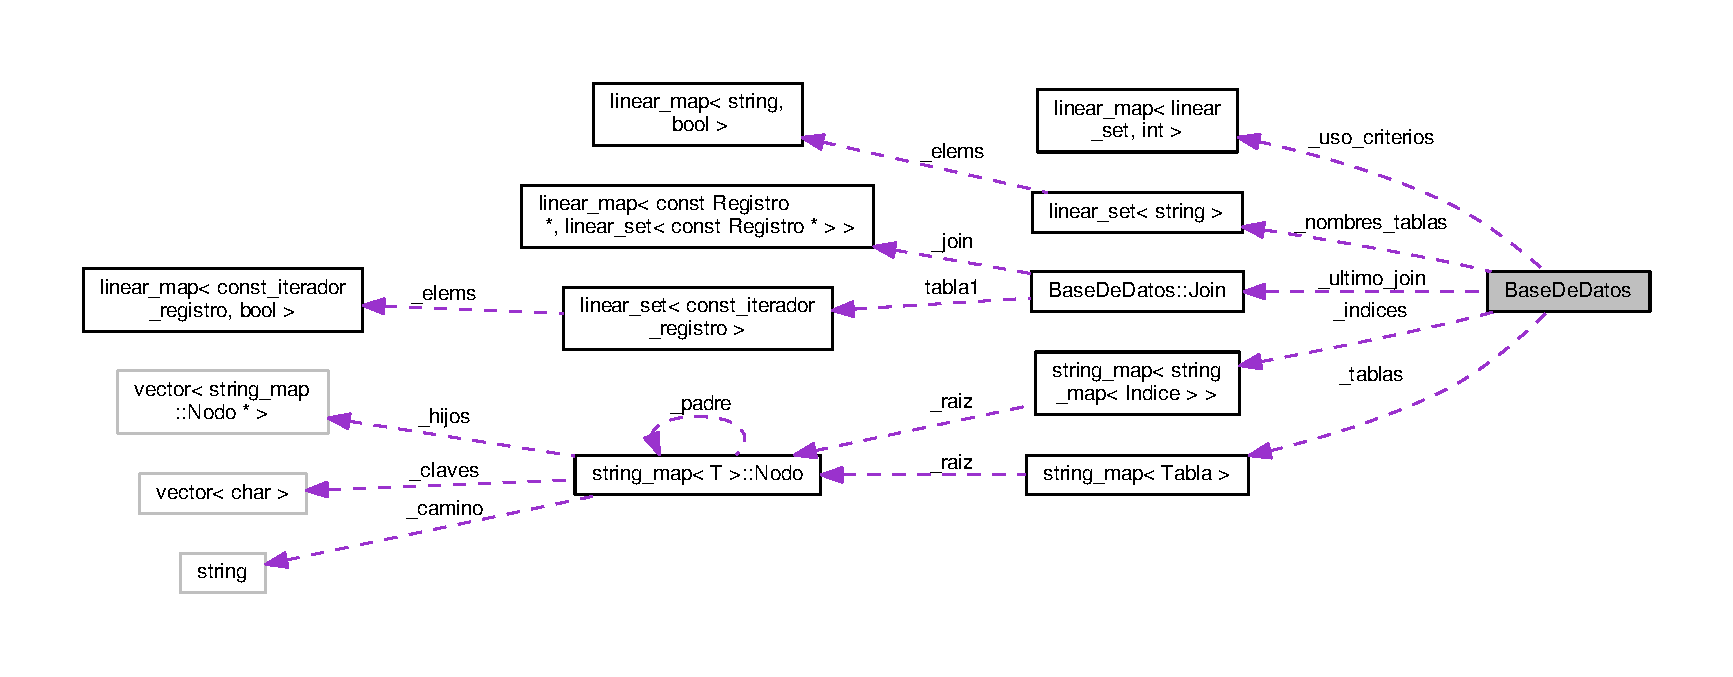
\includegraphics[width=350pt]{classBaseDeDatos__coll__graph}
\end{center}
\end{figure}
\subsection*{Tipos públicos}
\begin{DoxyCompactItemize}
\item 
\hypertarget{classBaseDeDatos_a6742a222e87623bc92a810a693fb337b}{typedef \hyperlink{classlinear__set}{linear\-\_\-set}$<$ \hyperlink{classRestriccion}{Restriccion} $>$ \hyperlink{classBaseDeDatos_a6742a222e87623bc92a810a693fb337b}{Criterio}}\label{classBaseDeDatos_a6742a222e87623bc92a810a693fb337b}

\begin{DoxyCompactList}\small\item\em Criterio de búsqueda para una base de datos. \end{DoxyCompactList}\item 
\hypertarget{classBaseDeDatos_a1e94d358c9ef6e71f9d6bfb662e553cb}{typedef \hyperlink{classlinear__map}{linear\-\_\-map}$<$ \hyperlink{classDato}{Dato}, \\*
\hyperlink{classlinear__set}{linear\-\_\-set}$<$ \hyperlink{classRegistro}{Registro} $>$ $>$ \hyperlink{classBaseDeDatos_a1e94d358c9ef6e71f9d6bfb662e553cb}{Indice}}\label{classBaseDeDatos_a1e94d358c9ef6e71f9d6bfb662e553cb}

\begin{DoxyCompactList}\small\item\em Indice es el dicc (\hyperlink{classDato}{Dato}, Conj (registro)) \end{DoxyCompactList}\end{DoxyCompactItemize}
\subsection*{Métodos públicos}
\begin{DoxyCompactItemize}
\item 
\hyperlink{classBaseDeDatos_a85a4992b2d9d7ed072efa792384495b5}{Base\-De\-Datos} ()
\begin{DoxyCompactList}\small\item\em Inicializa una base de datos sin tablas. \end{DoxyCompactList}\item 
void \hyperlink{classBaseDeDatos_aee0685f94a16b05b2893b24349716292}{crear\-Tabla} (const string \&nombre, const \hyperlink{classlinear__set}{linear\-\_\-set}$<$ string $>$ \&claves, const vector$<$ string $>$ \&campos, const vector$<$ \hyperlink{classDato}{Dato} $>$ \&tipos)
\begin{DoxyCompactList}\small\item\em Crea una nueva tabla en la base de datos. \end{DoxyCompactList}\item 
void \hyperlink{classBaseDeDatos_ada69808e7d6f26e34bab5b67ab4f5d05}{agregar\-Registro} (const \hyperlink{classRegistro}{Registro} \&r, const string \&nombre)
\begin{DoxyCompactList}\small\item\em Agrega un registro a la tabla parámetro. \end{DoxyCompactList}\item 
const \hyperlink{classlinear__set}{linear\-\_\-set}$<$ string $>$ \& \hyperlink{classBaseDeDatos_a24cb80244dbd9d34227f0d808aaeffa8}{tablas} () const 
\begin{DoxyCompactList}\small\item\em Devuelve el conjunto de tablas existentes en la base. \end{DoxyCompactList}\item 
const \hyperlink{classTabla}{Tabla} \& \hyperlink{classBaseDeDatos_ac83ffb074091a70f4879a85db830d603}{dame\-Tabla} (const string \&nombre) const 
\begin{DoxyCompactList}\small\item\em Devuelve la tabla asociada al nombre. \end{DoxyCompactList}\item 
int \hyperlink{classBaseDeDatos_a0b2094c4f3e59e38e5771b8d81da9077}{uso\-\_\-criterio} (const \hyperlink{classBaseDeDatos_a6742a222e87623bc92a810a693fb337b}{Criterio} \&criterio) const 
\begin{DoxyCompactList}\small\item\em Devuelve la cantidad de usos que tiene un criterio. \end{DoxyCompactList}\item 
bool \hyperlink{classBaseDeDatos_a451ef7b34a2ff9d395da10745266b703}{registro\-Valido} (const \hyperlink{classRegistro}{Registro} \&r, const string \&nombre) const 
\begin{DoxyCompactList}\small\item\em Evalúa si un registro puede ingresarse en la tabla parámetro. \end{DoxyCompactList}\item 
bool \hyperlink{classBaseDeDatos_a43f25f2c23796d5133c75f1973898b36}{criterio\-Valido} (const \hyperlink{classBaseDeDatos_a6742a222e87623bc92a810a693fb337b}{Criterio} \&c, const string \&nombre) const 
\begin{DoxyCompactList}\small\item\em Evalúa si un criterio puede aplicarse en la tabla parámetro. \end{DoxyCompactList}\item 
\hyperlink{classTabla}{Tabla} \hyperlink{classBaseDeDatos_aa0676f34e537e650095e55b3eef852cb}{busqueda} (const \hyperlink{classBaseDeDatos_a6742a222e87623bc92a810a693fb337b}{Criterio} \&c, const string \&nombre)
\begin{DoxyCompactList}\small\item\em Devuelve el resultado de buscar en una tabla con un criterio. \end{DoxyCompactList}\item 
\hyperlink{classlinear__set}{linear\-\_\-set}$<$ \hyperlink{classBaseDeDatos_a6742a222e87623bc92a810a693fb337b}{Criterio} $>$ \hyperlink{classBaseDeDatos_a907976b069e65a933e025035d887a3b5}{top\-\_\-criterios} () const 
\begin{DoxyCompactList}\small\item\em Devuelve los criterios de máximo uso. \end{DoxyCompactList}\end{DoxyCompactItemize}
\subsection*{Métodos privados}
{\bf }\par
\begin{DoxyCompactItemize}
\item 
bool \hyperlink{classBaseDeDatos_adf046a8fde5505668174122997ebb147}{\-\_\-mismos\-\_\-tipos} (const \hyperlink{classRegistro}{Registro} \&r, const \hyperlink{classTabla}{Tabla} \&t) const 
\begin{DoxyCompactList}\small\item\em Revisa si los campos del registro y la tabla tienen el mismo tipo. \end{DoxyCompactList}\item 
bool \hyperlink{classBaseDeDatos_a64ea8616111fb54b0804fe7560668ff6}{\-\_\-no\-\_\-repite} (const \hyperlink{classRegistro}{Registro} \&r, const \hyperlink{classTabla}{Tabla} \&t) const 
\begin{DoxyCompactList}\small\item\em Revisa si el registro no repite claves en la tabla. \end{DoxyCompactList}\item 
list$<$ \hyperlink{classRegistro}{Registro} $>$ \& \hyperlink{classBaseDeDatos_a14edefd67e0fca7c3f7f2e965424916a}{\-\_\-filtrar\-\_\-registros} (const string \&campo, const \hyperlink{classDato}{Dato} \&valor, list$<$ \hyperlink{classRegistro}{Registro} $>$ \&registros, bool igualdad) const 
\begin{DoxyCompactList}\small\item\em Filtra la lista de registros parametro según el criterio. \end{DoxyCompactList}\item 
list$<$ \hyperlink{classRegistro}{Registro} $>$ \& \hyperlink{classBaseDeDatos_ab64f6c5aed35a029620da579853733ba}{\-\_\-filtrar\-\_\-registros} (const string \&campo, const \hyperlink{classDato}{Dato} \&valor, list$<$ \hyperlink{classRegistro}{Registro} $>$ \&registros) const 
\begin{DoxyCompactList}\small\item\em Filtra la lista de registros parametro según el criterio. \end{DoxyCompactList}\item 
pair$<$ vector$<$ string $>$, vector\\*
$<$ \hyperlink{classDato}{Dato} $>$ $>$ \hyperlink{classBaseDeDatos_ad5b99bf20095789ca5636bf0593ad8a5}{\-\_\-tipos\-\_\-tabla} (const \hyperlink{classTabla}{Tabla} \&t)
\begin{DoxyCompactList}\small\item\em Obtiene los campos y tipos de una tabla. \end{DoxyCompactList}\end{DoxyCompactItemize}

\subsection*{Atributos privados}
\begin{Indent}{\bf Representación}\par
{\em rep\-: basededatos $\to$ bool\par
rep(bd) $\equiv$
\begin{DoxyItemize}
\item \-\_\-nombres\-\_\-tablas = claves(\-\_\-tablas) $\land$
\item $\forall$ (c \-: Criterio) c $\in$ claves(\-\_\-uso\-\_\-criterios) $\Rightarrow$
\begin{DoxyItemize}
\item (
\begin{DoxyItemize}
\item $\exists$ (n \-: string) n $\in$ \-\_\-nombres\-\_\-tablas
\item $\land$ criterio\-Valido(c, n, db)
\end{DoxyItemize}
\item ) $\land$
\item obtener(c, \-\_\-uso\-\_\-criterios) $>$ 0
\end{DoxyItemize}
\end{DoxyItemize}

$\forall$ (t \-: string) def?(t , \-\_\-indices) $\Rightarrow$ def?(t , \-\_\-tablas) $\land$
\begin{DoxyItemize}
\item $\lnot$ vacio?(claves(obtener(t, \-\_\-indices))) $\land$
\item (
\begin{DoxyItemize}
\item $\forall$ (c \-: string) def? (c , obtener(t , \-\_\-indices)) $\Rightarrow$
\begin{DoxyItemize}
\item c $\in$ campos(obtener(t , \-\_\-tablas)) $\land$
\item (
\begin{DoxyItemize}
\item $\forall$ (d \-: \hyperlink{classDato}{Dato}) def?(d, obtener(c, obtener(t , \-\_\-indices))) $\Rightarrow$
\begin{DoxyItemize}
\item $\lnot$ vacio?(obtener(d, obtener(c, obtener(t , \-\_\-indices)))) $\land$
\item (
\begin{DoxyItemize}
\item $\forall$ (r \-: \hyperlink{classRegistro}{Registro}) r $\in$ obtener(d, obtener(c, obtener(t , \-\_\-indices))) $\Rightarrow$
\begin{DoxyItemize}
\item r $\in$ registros (obtener(t, \-\_\-tablas)) $\land$ valor(c, r) = d
\end{DoxyItemize}
\end{DoxyItemize}
\item )
\end{DoxyItemize}
\end{DoxyItemize}
\item )
\end{DoxyItemize}
\end{DoxyItemize}
\item )
\end{DoxyItemize}

abs\-: basededatos $\to$ \hyperlink{classBaseDeDatos}{Base\-De\-Datos}\par
abs(bd) $\equiv$ bd' $|$
\begin{DoxyItemize}
\item \-\_\-nombres\-\_\-tablas = tablas(bd') $\land$
\item ( $\forall$ nt \-: string) nt $\in$ \-\_\-nombres\-\_\-tablas $\Rightarrow$
\begin{DoxyItemize}
\item obtener(nt, \-\_\-tablas) = dame\-Tabla(nt, bd') $\land$
\end{DoxyItemize}
\item ( $\forall$ c \-: criterio)
\begin{DoxyItemize}
\item (uso\-Criterio(c, bd') == 0 $\land$ $\lnot$ def?(c, \-\_\-uso\-\_\-criterios)) $\lor$
\item (uso\-Criterio(c, db') == obtener(c, \-\_\-uso\-\_\-criterios)) $\land$
\end{DoxyItemize}
\item ( $\forall$ t \-: string) t $\in$ tablas(bd') $\land$
\item ( $\forall$ c \-: string) c $\in$ campos(dame\-Tabla(t, bd'))
\begin{DoxyItemize}
\item tiene\-Indice?(t, c, bd') == def?(c, obtener(t, \-\_\-indices)) 
\end{DoxyItemize}
\end{DoxyItemize}}\begin{DoxyCompactItemize}
\item 
\hypertarget{classBaseDeDatos_ae93f3d0a8d138e5742c52b9f2294d2bd}{\hyperlink{classlinear__set}{linear\-\_\-set}$<$ string $>$ {\bfseries \-\_\-nombres\-\_\-tablas}}\label{classBaseDeDatos_ae93f3d0a8d138e5742c52b9f2294d2bd}

\item 
\hypertarget{classBaseDeDatos_abc71fb94bf17d92df678705224cfd9b0}{\hyperlink{classlinear__map}{linear\-\_\-map}$<$ string, \hyperlink{classTabla}{Tabla} $>$ {\bfseries \-\_\-tablas}}\label{classBaseDeDatos_abc71fb94bf17d92df678705224cfd9b0}

\item 
\hypertarget{classBaseDeDatos_acc03ee648f19ad950d399861cc263a30}{\hyperlink{classlinear__map}{linear\-\_\-map}$<$ \hyperlink{classBaseDeDatos_a6742a222e87623bc92a810a693fb337b}{Criterio}, int $>$ {\bfseries \-\_\-uso\-\_\-criterios}}\label{classBaseDeDatos_acc03ee648f19ad950d399861cc263a30}

\item 
\hypertarget{classBaseDeDatos_adb2234a6b0c8cb3b0b503f3e48cc3cc5}{\hyperlink{classlinear__map}{linear\-\_\-map}$<$ string, \hyperlink{classlinear__map}{linear\-\_\-map}\\*
$<$ string, \hyperlink{classBaseDeDatos_a1e94d358c9ef6e71f9d6bfb662e553cb}{Indice} $>$ $>$ {\bfseries \-\_\-indices}}\label{classBaseDeDatos_adb2234a6b0c8cb3b0b503f3e48cc3cc5}

\end{DoxyCompactItemize}
\end{Indent}


\subsection{Descripción detallada}
Una base de datos es un administrador de tablas con funciones de búsqueda. 

Una base de datos permite administrar tablas identificadas por registro. Permite saber si se puede agegar un registro a una tabla y luego agregarlo. Permite realizar filtros del contenido de tablas mediante criterios de búsqueda. Además mantiene estadísticas del uso de los criterios.

{\bfseries se explica con} T\-A\-D \hyperlink{classBaseDeDatos}{Base\-De\-Datos} 

\subsection{Documentación del constructor y destructor}
\hypertarget{classBaseDeDatos_a85a4992b2d9d7ed072efa792384495b5}{\index{Base\-De\-Datos@{Base\-De\-Datos}!Base\-De\-Datos@{Base\-De\-Datos}}
\index{Base\-De\-Datos@{Base\-De\-Datos}!BaseDeDatos@{Base\-De\-Datos}}
\subsubsection[{Base\-De\-Datos}]{\setlength{\rightskip}{0pt plus 5cm}Base\-De\-Datos\-::\-Base\-De\-Datos (
\begin{DoxyParamCaption}
{}
\end{DoxyParamCaption}
)}}\label{classBaseDeDatos_a85a4992b2d9d7ed072efa792384495b5}


Inicializa una base de datos sin tablas. 

\begin{DoxyPrecond}{Precondición}
true 
\end{DoxyPrecond}
\begin{DoxyPostcond}{Postcondición}
{\bfseries this} = nueva\-D\-B
\end{DoxyPostcond}

\begin{DoxyDescription}
\item[Complejidad Temporal]$O$(1)
\end{DoxyDescription}

\subsection{Documentación de las funciones miembro}
\hypertarget{classBaseDeDatos_a14edefd67e0fca7c3f7f2e965424916a}{\index{Base\-De\-Datos@{Base\-De\-Datos}!\-\_\-filtrar\-\_\-registros@{\-\_\-filtrar\-\_\-registros}}
\index{\-\_\-filtrar\-\_\-registros@{\-\_\-filtrar\-\_\-registros}!BaseDeDatos@{Base\-De\-Datos}}
\subsubsection[{\-\_\-filtrar\-\_\-registros}]{\setlength{\rightskip}{0pt plus 5cm}list$<$ {\bf Registro} $>$ \& Base\-De\-Datos\-::\-\_\-filtrar\-\_\-registros (
\begin{DoxyParamCaption}
\item[{const string \&}]{campo, }
\item[{const {\bf Dato} \&}]{valor, }
\item[{list$<$ {\bf Registro} $>$ \&}]{registros, }
\item[{bool}]{igualdad}
\end{DoxyParamCaption}
) const\hspace{0.3cm}{\ttfamily [private]}}}\label{classBaseDeDatos_a14edefd67e0fca7c3f7f2e965424916a}


Filtra la lista de registros parametro según el criterio. 

El resultado tiene aliasing con el parámetro registros.

\begin{DoxyPrecond}{Precondición}
$\forall$ (r \-: \hyperlink{classRegistro}{Registro}) r $\in$ registros $\Rightarrow$ campo $\in$ campos(r) $\land$ tipo?(valor(campo, r)) = tipo?(valor) 
\end{DoxyPrecond}
\begin{DoxyPostcond}{Postcondición}
{\bfseries res} = filtrar\-Registros\-Segun\-Restriccion( nueva(campo, valor, igualdad), registros) 
\end{DoxyPostcond}
\hypertarget{classBaseDeDatos_ab64f6c5aed35a029620da579853733ba}{\index{Base\-De\-Datos@{Base\-De\-Datos}!\-\_\-filtrar\-\_\-registros@{\-\_\-filtrar\-\_\-registros}}
\index{\-\_\-filtrar\-\_\-registros@{\-\_\-filtrar\-\_\-registros}!BaseDeDatos@{Base\-De\-Datos}}
\subsubsection[{\-\_\-filtrar\-\_\-registros}]{\setlength{\rightskip}{0pt plus 5cm}list$<$ {\bf Registro} $>$ \& Base\-De\-Datos\-::\-\_\-filtrar\-\_\-registros (
\begin{DoxyParamCaption}
\item[{const string \&}]{campo, }
\item[{const {\bf Dato} \&}]{valor, }
\item[{list$<$ {\bf Registro} $>$ \&}]{registros}
\end{DoxyParamCaption}
) const\hspace{0.3cm}{\ttfamily [private]}}}\label{classBaseDeDatos_ab64f6c5aed35a029620da579853733ba}


Filtra la lista de registros parametro según el criterio. 

El resultado tiene aliasing con el parámetro registros.

\begin{DoxyPrecond}{Precondición}
$\forall$ (r \-: \hyperlink{classRegistro}{Registro}) r $\in$ registros $\Rightarrow$ campo $\in$ campos(r) $\land$ tipo?(valor(campo, r)) = tipo?(valor) 
\end{DoxyPrecond}
\begin{DoxyPostcond}{Postcondición}
{\bfseries res} = filtrar\-Registros\-Segun\-Restriccion( nueva(campo, valor, true), registros) 
\end{DoxyPostcond}
\hypertarget{classBaseDeDatos_adf046a8fde5505668174122997ebb147}{\index{Base\-De\-Datos@{Base\-De\-Datos}!\-\_\-mismos\-\_\-tipos@{\-\_\-mismos\-\_\-tipos}}
\index{\-\_\-mismos\-\_\-tipos@{\-\_\-mismos\-\_\-tipos}!BaseDeDatos@{Base\-De\-Datos}}
\subsubsection[{\-\_\-mismos\-\_\-tipos}]{\setlength{\rightskip}{0pt plus 5cm}bool Base\-De\-Datos\-::\-\_\-mismos\-\_\-tipos (
\begin{DoxyParamCaption}
\item[{const {\bf Registro} \&}]{r, }
\item[{const {\bf Tabla} \&}]{t}
\end{DoxyParamCaption}
) const\hspace{0.3cm}{\ttfamily [private]}}}\label{classBaseDeDatos_adf046a8fde5505668174122997ebb147}


Revisa si los campos del registro y la tabla tienen el mismo tipo. 

\begin{DoxyPrecond}{Precondición}
campos(r) == campos(t) 
\end{DoxyPrecond}
\begin{DoxyPostcond}{Postcondición}
{\bfseries res} == $\forall$ (c \-: campo) c $\in$ campos(r) $\Rightarrow$ Nat?(valor(c, r)) == tipo\-Campo(c, t)
\end{DoxyPostcond}

\begin{DoxyDescription}
\item[Complejidad Temporal]O(\-C$^\wedge$2)
\end{DoxyDescription}\hypertarget{classBaseDeDatos_a64ea8616111fb54b0804fe7560668ff6}{\index{Base\-De\-Datos@{Base\-De\-Datos}!\-\_\-no\-\_\-repite@{\-\_\-no\-\_\-repite}}
\index{\-\_\-no\-\_\-repite@{\-\_\-no\-\_\-repite}!BaseDeDatos@{Base\-De\-Datos}}
\subsubsection[{\-\_\-no\-\_\-repite}]{\setlength{\rightskip}{0pt plus 5cm}bool Base\-De\-Datos\-::\-\_\-no\-\_\-repite (
\begin{DoxyParamCaption}
\item[{const {\bf Registro} \&}]{r, }
\item[{const {\bf Tabla} \&}]{t}
\end{DoxyParamCaption}
) const\hspace{0.3cm}{\ttfamily [private]}}}\label{classBaseDeDatos_a64ea8616111fb54b0804fe7560668ff6}


Revisa si el registro no repite claves en la tabla. 

\begin{DoxyPrecond}{Precondición}
compatible(r, t) 
\end{DoxyPrecond}
\begin{DoxyPostcond}{Postcondición}
{\bfseries res} = $\forall$ (r' \-: \hyperlink{classRegistro}{Registro}) r $\in$ registros(t) $\Rightarrow$ $\exists$ (c \-: campo) c $\in$ claves(t) $\land$ valor(c, r') != valor(c, r)
\end{DoxyPostcond}

\begin{DoxyDescription}
\item[Complejidad Temporal]O(c $\ast$ C + c $\ast$ n $\ast$ (C + L))
\end{DoxyDescription}\hypertarget{classBaseDeDatos_ad5b99bf20095789ca5636bf0593ad8a5}{\index{Base\-De\-Datos@{Base\-De\-Datos}!\-\_\-tipos\-\_\-tabla@{\-\_\-tipos\-\_\-tabla}}
\index{\-\_\-tipos\-\_\-tabla@{\-\_\-tipos\-\_\-tabla}!BaseDeDatos@{Base\-De\-Datos}}
\subsubsection[{\-\_\-tipos\-\_\-tabla}]{\setlength{\rightskip}{0pt plus 5cm}pair$<$ vector$<$ string $>$, vector$<$ {\bf Dato} $>$ $>$ Base\-De\-Datos\-::\-\_\-tipos\-\_\-tabla (
\begin{DoxyParamCaption}
\item[{const {\bf Tabla} \&}]{t}
\end{DoxyParamCaption}
)\hspace{0.3cm}{\ttfamily [private]}}}\label{classBaseDeDatos_ad5b99bf20095789ca5636bf0593ad8a5}


Obtiene los campos y tipos de una tabla. 

\begin{DoxyPrecond}{Precondición}
true 
\end{DoxyPrecond}
\begin{DoxyPostcond}{Postcondición}
( $\forall$ (c \-: Campo) está?(c, $\pi_1$({\bfseries res})) $\Leftrightarrow$ c $\in$ campos(t)) $\land$ \#(campos(t)) = long( $\pi_1$({\bfseries res})) $\land$ $\forall$ (i \-: Nat) 0 $\leq$ i $<$ \#(campos(t)) $\Rightarrow$ tipo?( $\pi_2$({\bfseries res})\mbox{[}i\mbox{]}) = tipo\-Campo( $\pi_1$({\bfseries res})\mbox{[}i\mbox{]}, t) 
\end{DoxyPostcond}
\hypertarget{classBaseDeDatos_ada69808e7d6f26e34bab5b67ab4f5d05}{\index{Base\-De\-Datos@{Base\-De\-Datos}!agregar\-Registro@{agregar\-Registro}}
\index{agregar\-Registro@{agregar\-Registro}!BaseDeDatos@{Base\-De\-Datos}}
\subsubsection[{agregar\-Registro}]{\setlength{\rightskip}{0pt plus 5cm}void Base\-De\-Datos\-::agregar\-Registro (
\begin{DoxyParamCaption}
\item[{const {\bf Registro} \&}]{r, }
\item[{const string \&}]{nombre}
\end{DoxyParamCaption}
)}}\label{classBaseDeDatos_ada69808e7d6f26e34bab5b67ab4f5d05}


Agrega un registro a la tabla parámetro. 


\begin{DoxyParams}{Parámetros}
{\em r} & \hyperlink{classRegistro}{Registro} a agregar \\
\hline
{\em nombre} & Nombre de la tabla donde se agrega el registro\\
\hline
\end{DoxyParams}
\begin{DoxyPrecond}{Precondición}
db = {\bfseries this} $\land$ nombre $\in$ tablas({\bfseries this}) $\land$ puedo\-Insertar?(r, dame\-Tabla({\bfseries this})) 
\end{DoxyPrecond}
\begin{DoxyPostcond}{Postcondición}
{\bfseries this} = insertar\-Entrada(r, nombre, db)
\end{DoxyPostcond}

\begin{DoxyDescription}
\item[Complejidad Temporal]$O$(T + copy(reg))
\end{DoxyDescription}\hypertarget{classBaseDeDatos_aa0676f34e537e650095e55b3eef852cb}{\index{Base\-De\-Datos@{Base\-De\-Datos}!busqueda@{busqueda}}
\index{busqueda@{busqueda}!BaseDeDatos@{Base\-De\-Datos}}
\subsubsection[{busqueda}]{\setlength{\rightskip}{0pt plus 5cm}{\bf Tabla} Base\-De\-Datos\-::busqueda (
\begin{DoxyParamCaption}
\item[{const {\bf Criterio} \&}]{c, }
\item[{const string \&}]{nombre}
\end{DoxyParamCaption}
)}}\label{classBaseDeDatos_aa0676f34e537e650095e55b3eef852cb}


Devuelve el resultado de buscar en una tabla con un criterio. 


\begin{DoxyParams}{Parámetros}
{\em c} & Criterio de búsqueda utilizado. \\
\hline
{\em nombre} & Nombre de la tabla.\\
\hline
\end{DoxyParams}
\begin{DoxyPrecond}{Precondición}
nombre $\in$ tablas({\bfseries this}) $\land$ criterio\-Valido(c, nombre, {\bfseries this}) 
\end{DoxyPrecond}
\begin{DoxyPostcond}{Postcondición}
{\bfseries res} = buscar(c, nombre, {\bfseries this})
\end{DoxyPostcond}

\begin{DoxyDescription}
\item[Complejidad Temporal]$O$(T + cs $\ast$ cmp(\-Criterio) + cr $\ast$ n $\ast$ (C + L + copy(reg)))
\end{DoxyDescription}\hypertarget{classBaseDeDatos_aee0685f94a16b05b2893b24349716292}{\index{Base\-De\-Datos@{Base\-De\-Datos}!crear\-Tabla@{crear\-Tabla}}
\index{crear\-Tabla@{crear\-Tabla}!BaseDeDatos@{Base\-De\-Datos}}
\subsubsection[{crear\-Tabla}]{\setlength{\rightskip}{0pt plus 5cm}void Base\-De\-Datos\-::crear\-Tabla (
\begin{DoxyParamCaption}
\item[{const string \&}]{nombre, }
\item[{const {\bf linear\-\_\-set}$<$ string $>$ \&}]{claves, }
\item[{const vector$<$ string $>$ \&}]{campos, }
\item[{const vector$<$ {\bf Dato} $>$ \&}]{tipos}
\end{DoxyParamCaption}
)}}\label{classBaseDeDatos_aee0685f94a16b05b2893b24349716292}


Crea una nueva tabla en la base de datos. 


\begin{DoxyParams}{Parámetros}
{\em nombre} & Nombre identificador de la tabla \\
\hline
{\em claves} & Claves de la tabla a crear \\
\hline
{\em campos} & Campos de la tabla a crear \\
\hline
{\em tipos} & Tipos para los campos de la tabla a crear\\
\hline
\end{DoxyParams}
\begin{DoxyPrecond}{Precondición}
db = {\bfseries this} $\land$ $\lnot$ (nombre $\in$ tablas({\bfseries this})) $\land$ $\land$ $\lnot$ $\emptyset$?(claves) $\land$ $\forall$ (c\-: campo) c $\in$ claves  c $\in$ campos $\land$ long(campos) = long(tipos) $\land$ sin\-Repetidos(campos) 
\end{DoxyPrecond}
\begin{DoxyPostcond}{Postcondición}
{\bfseries this} = agregar\-Tabla(nueva\-Tabla(claves, nuevo\-Registro(campos, tipos)), db)
\end{DoxyPostcond}

\begin{DoxyDescription}
\item[Complejidad Temporal]$O$(C)
\end{DoxyDescription}\hypertarget{classBaseDeDatos_a43f25f2c23796d5133c75f1973898b36}{\index{Base\-De\-Datos@{Base\-De\-Datos}!criterio\-Valido@{criterio\-Valido}}
\index{criterio\-Valido@{criterio\-Valido}!BaseDeDatos@{Base\-De\-Datos}}
\subsubsection[{criterio\-Valido}]{\setlength{\rightskip}{0pt plus 5cm}bool Base\-De\-Datos\-::criterio\-Valido (
\begin{DoxyParamCaption}
\item[{const {\bf Criterio} \&}]{c, }
\item[{const string \&}]{nombre}
\end{DoxyParamCaption}
) const}}\label{classBaseDeDatos_a43f25f2c23796d5133c75f1973898b36}


Evalúa si un criterio puede aplicarse en la tabla parámetro. 


\begin{DoxyParams}{Parámetros}
{\em c} & Criterio a utilizar. \\
\hline
{\em nombre} & Nombre de la tabla.\\
\hline
\end{DoxyParams}
\begin{DoxyPrecond}{Precondición}
tabla $\in$ tablas({\bfseries this}) 
\end{DoxyPrecond}
\begin{DoxyPostcond}{Postcondición}
{\bfseries res} = criterio\-Valido(c, nombre, {\bfseries this})
\end{DoxyPostcond}

\begin{DoxyDescription}
\item[Complejidad Temporal]$O$(T + cr $\ast$ C)
\end{DoxyDescription}\hypertarget{classBaseDeDatos_ac83ffb074091a70f4879a85db830d603}{\index{Base\-De\-Datos@{Base\-De\-Datos}!dame\-Tabla@{dame\-Tabla}}
\index{dame\-Tabla@{dame\-Tabla}!BaseDeDatos@{Base\-De\-Datos}}
\subsubsection[{dame\-Tabla}]{\setlength{\rightskip}{0pt plus 5cm}const {\bf Tabla} \& Base\-De\-Datos\-::dame\-Tabla (
\begin{DoxyParamCaption}
\item[{const string \&}]{nombre}
\end{DoxyParamCaption}
) const}}\label{classBaseDeDatos_ac83ffb074091a70f4879a85db830d603}


Devuelve la tabla asociada al nombre. 

La tabla se devuelve por referencia no modificable.


\begin{DoxyParams}{Parámetros}
{\em nombre} & Nombre de la tabla buscada.\\
\hline
\end{DoxyParams}
\begin{DoxyPrecond}{Precondición}
nombre $\in$ tablas({\bfseries this}) 
\end{DoxyPrecond}
\begin{DoxyPostcond}{Postcondición}
{\bfseries res} = dame\-Tabla(nombre, {\bfseries this})
\end{DoxyPostcond}

\begin{DoxyDescription}
\item[Complejidad Temporal]O(\-T)
\end{DoxyDescription}\hypertarget{classBaseDeDatos_a451ef7b34a2ff9d395da10745266b703}{\index{Base\-De\-Datos@{Base\-De\-Datos}!registro\-Valido@{registro\-Valido}}
\index{registro\-Valido@{registro\-Valido}!BaseDeDatos@{Base\-De\-Datos}}
\subsubsection[{registro\-Valido}]{\setlength{\rightskip}{0pt plus 5cm}bool Base\-De\-Datos\-::registro\-Valido (
\begin{DoxyParamCaption}
\item[{const {\bf Registro} \&}]{r, }
\item[{const string \&}]{nombre}
\end{DoxyParamCaption}
) const}}\label{classBaseDeDatos_a451ef7b34a2ff9d395da10745266b703}


Evalúa si un registro puede ingresarse en la tabla parámetro. 


\begin{DoxyParams}{Parámetros}
{\em r} & \hyperlink{classRegistro}{Registro} a ingresar en la tabla. \\
\hline
{\em nombre} & Nombre de la tabla.\\
\hline
\end{DoxyParams}
\begin{DoxyPrecond}{Precondición}
nombre $\in$ tablas({\bfseries this}) 
\end{DoxyPrecond}
\begin{DoxyPostcond}{Postcondición}
{\bfseries res} = puedo\-Insertar?(r, dame\-Tabla(nombre, {\bfseries this}))
\end{DoxyPostcond}

\begin{DoxyDescription}
\item[Complejidad Temporal]$O$(T + C$^\wedge$2 + (c $\ast$ C + c $\ast$ n $\ast$ (C + L)))
\end{DoxyDescription}\hypertarget{classBaseDeDatos_a24cb80244dbd9d34227f0d808aaeffa8}{\index{Base\-De\-Datos@{Base\-De\-Datos}!tablas@{tablas}}
\index{tablas@{tablas}!BaseDeDatos@{Base\-De\-Datos}}
\subsubsection[{tablas}]{\setlength{\rightskip}{0pt plus 5cm}const {\bf linear\-\_\-set}$<$ string $>$ \& Base\-De\-Datos\-::tablas (
\begin{DoxyParamCaption}
{}
\end{DoxyParamCaption}
) const}}\label{classBaseDeDatos_a24cb80244dbd9d34227f0d808aaeffa8}


Devuelve el conjunto de tablas existentes en la base. 

El conjunto de nombres se devuelve por referencia no-\/modificable.

\begin{DoxyPrecond}{Precondición}
true 
\end{DoxyPrecond}
\begin{DoxyPostcond}{Postcondición}
{\bfseries res} = tablas({\bfseries this})
\end{DoxyPostcond}

\begin{DoxyDescription}
\item[Complejidad Temporal]$O$(1)
\end{DoxyDescription}\hypertarget{classBaseDeDatos_a907976b069e65a933e025035d887a3b5}{\index{Base\-De\-Datos@{Base\-De\-Datos}!top\-\_\-criterios@{top\-\_\-criterios}}
\index{top\-\_\-criterios@{top\-\_\-criterios}!BaseDeDatos@{Base\-De\-Datos}}
\subsubsection[{top\-\_\-criterios}]{\setlength{\rightskip}{0pt plus 5cm}{\bf linear\-\_\-set}$<$ {\bf Base\-De\-Datos\-::\-Criterio} $>$ Base\-De\-Datos\-::top\-\_\-criterios (
\begin{DoxyParamCaption}
{}
\end{DoxyParamCaption}
) const}}\label{classBaseDeDatos_a907976b069e65a933e025035d887a3b5}


Devuelve los criterios de máximo uso. 

\begin{DoxyPrecond}{Precondición}
true 
\end{DoxyPrecond}
\begin{DoxyPostcond}{Postcondición}
$\forall$ (c \-: Criterio) \mbox{[}c $\in$ {\bfseries res} $\Leftrightarrow$ $\forall$ (c' \-: Criterio) uso\-Criterio(c, db) $>$= uso\-Criterio(c', db)\mbox{]}
\end{DoxyPostcond}

\begin{DoxyDescription}
\item[Complejidad Temporal]$O$(cs $\ast$ copy(\-Criterio))
\end{DoxyDescription}\hypertarget{classBaseDeDatos_a0b2094c4f3e59e38e5771b8d81da9077}{\index{Base\-De\-Datos@{Base\-De\-Datos}!uso\-\_\-criterio@{uso\-\_\-criterio}}
\index{uso\-\_\-criterio@{uso\-\_\-criterio}!BaseDeDatos@{Base\-De\-Datos}}
\subsubsection[{uso\-\_\-criterio}]{\setlength{\rightskip}{0pt plus 5cm}int Base\-De\-Datos\-::uso\-\_\-criterio (
\begin{DoxyParamCaption}
\item[{const {\bf Criterio} \&}]{criterio}
\end{DoxyParamCaption}
) const}}\label{classBaseDeDatos_a0b2094c4f3e59e38e5771b8d81da9077}


Devuelve la cantidad de usos que tiene un criterio. 


\begin{DoxyParams}{Parámetros}
{\em criterio} & Criterio por el cual se consulta.\\
\hline
\end{DoxyParams}
\begin{DoxyPrecond}{Precondición}
nombre $\in$ tablas({\bfseries this}) 
\end{DoxyPrecond}
\begin{DoxyPostcond}{Postcondición}
{\bfseries res} = uso\-Criterio(criterio, {\bfseries this})
\end{DoxyPostcond}

\begin{DoxyDescription}
\item[Complejidad Temporal]$O$(\#cs $\ast$ cmp(\-Criterio))
\end{DoxyDescription}

La documentación para esta clase fue generada a partir de los siguientes ficheros\-:\begin{DoxyCompactItemize}
\item 
src/Base\-De\-Datos.\-h\item 
src/Base\-De\-Datos.\-cpp\end{DoxyCompactItemize}

\hypertarget{classTabla_1_1const__iterador__registros}{\section{Referencia de la Clase Tabla\-:\-:const\-\_\-iterador\-\_\-registros}
\label{classTabla_1_1const__iterador__registros}\index{Tabla\-::const\-\_\-iterador\-\_\-registros@{Tabla\-::const\-\_\-iterador\-\_\-registros}}
}


Iterador de los registros de una tabla.  




{\ttfamily \#include $<$const\-\_\-iterador\-\_\-registros.\-h$>$}



Diagrama de colaboración para Tabla\-:\-:const\-\_\-iterador\-\_\-registros\-:\nopagebreak
\begin{figure}[H]
\begin{center}
\leavevmode
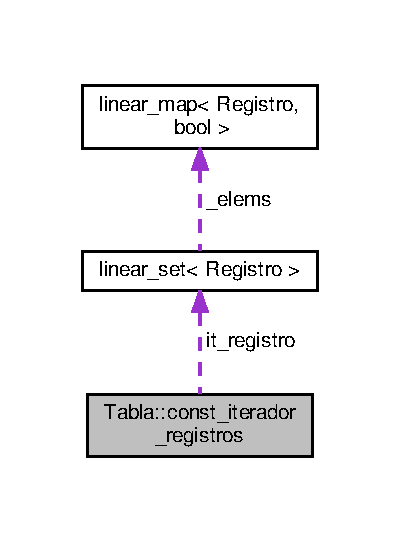
\includegraphics[width=192pt]{classTabla_1_1const__iterador__registros__coll__graph}
\end{center}
\end{figure}
\subsection*{Métodos públicos}
\begin{DoxyCompactItemize}
\item 
\hyperlink{classTabla_1_1const__iterador__registros_a904a84af50ced6c3d9e77e10d6e5192a}{const\-\_\-iterador\-\_\-registros} (const \hyperlink{classTabla_1_1const__iterador__registros}{const\-\_\-iterador\-\_\-registros} \&o\-\_\-it)
\begin{DoxyCompactList}\small\item\em Constructor por copia del iterador. \end{DoxyCompactList}\item 
const \hyperlink{classRegistro}{Registro} \& \hyperlink{classTabla_1_1const__iterador__registros_ae09f1cd7f790f7b3d9cb392a6f8ebbe5}{operator$\ast$} () const 
\begin{DoxyCompactList}\small\item\em Desreferencia el puntero. \end{DoxyCompactList}\item 
const \hyperlink{classRegistro}{Registro} $\ast$ \hyperlink{classTabla_1_1const__iterador__registros_aca0f97220fabe6bf6f822f1b217c76d5}{operator-\/$>$} () const 
\begin{DoxyCompactList}\small\item\em Operador flechita. \end{DoxyCompactList}\item 
\hyperlink{classTabla_1_1const__iterador__registros}{const\-\_\-iterador\-\_\-registros} \& \hyperlink{classTabla_1_1const__iterador__registros_a396373a330a7c56e3112df2bcccef885}{operator++} ()
\begin{DoxyCompactList}\small\item\em Avanza el iterador una posición. \end{DoxyCompactList}\item 
bool \hyperlink{classTabla_1_1const__iterador__registros_a97bb754644a0761f832bb858df07b2ff}{operator==} (const \hyperlink{classTabla_1_1const__iterador__registros}{const\-\_\-iterador\-\_\-registros} \&o\-\_\-it) const 
\begin{DoxyCompactList}\small\item\em Comparación entre iteradores. \end{DoxyCompactList}\item 
bool \hyperlink{classTabla_1_1const__iterador__registros_a042b2cc92666f899b9b503327f84b7ac}{operator!=} (const \hyperlink{classTabla_1_1const__iterador__registros}{const\-\_\-iterador\-\_\-registros} \&o\-\_\-it) const 
\begin{DoxyCompactList}\small\item\em Comparación entre iteradores. \end{DoxyCompactList}\end{DoxyCompactItemize}
\subsection*{Métodos privados}
\begin{DoxyCompactItemize}
\item 
\hypertarget{classTabla_1_1const__iterador__registros_a8dde708af2d71cf5dabfd3b42d15284f}{{\bfseries const\-\_\-iterador\-\_\-registros} (const \hyperlink{classlinear__set}{linear\-\_\-set}$<$ \hyperlink{classRegistro}{Registro} $>$\-::const\-\_\-iterator)}\label{classTabla_1_1const__iterador__registros_a8dde708af2d71cf5dabfd3b42d15284f}

\end{DoxyCompactItemize}
\subsection*{Atributos privados}
\begin{DoxyCompactItemize}
\item 
\hypertarget{classTabla_1_1const__iterador__registros_ab650d9f113456460fca266d31dffa484}{\hyperlink{classlinear__set}{linear\-\_\-set}$<$ \hyperlink{classRegistro}{Registro} $>$\\*
\-::const\-\_\-iterator {\bfseries it\-\_\-registro}}\label{classTabla_1_1const__iterador__registros_ab650d9f113456460fca266d31dffa484}

\end{DoxyCompactItemize}
\subsection*{Amigas}
\begin{DoxyCompactItemize}
\item 
\hypertarget{classTabla_1_1const__iterador__registros_a172484163cb8b80140c3053a4c68e4da}{class {\bfseries Tabla}}\label{classTabla_1_1const__iterador__registros_a172484163cb8b80140c3053a4c68e4da}

\end{DoxyCompactItemize}


\subsection{Descripción detallada}
Iterador de los registros de una tabla. 

\subsection{Documentación del constructor y destructor}
\hypertarget{classTabla_1_1const__iterador__registros_a904a84af50ced6c3d9e77e10d6e5192a}{\index{Tabla\-::const\-\_\-iterador\-\_\-registros@{Tabla\-::const\-\_\-iterador\-\_\-registros}!const\-\_\-iterador\-\_\-registros@{const\-\_\-iterador\-\_\-registros}}
\index{const\-\_\-iterador\-\_\-registros@{const\-\_\-iterador\-\_\-registros}!Tabla::const_iterador_registros@{Tabla\-::const\-\_\-iterador\-\_\-registros}}
\subsubsection[{const\-\_\-iterador\-\_\-registros}]{\setlength{\rightskip}{0pt plus 5cm}Tabla\-::const\-\_\-iterador\-\_\-registros\-::const\-\_\-iterador\-\_\-registros (
\begin{DoxyParamCaption}
\item[{const {\bf const\-\_\-iterador\-\_\-registros} \&}]{o\-\_\-it}
\end{DoxyParamCaption}
)}}\label{classTabla_1_1const__iterador__registros_a904a84af50ced6c3d9e77e10d6e5192a}


Constructor por copia del iterador. 


\begin{DoxyDescription}
\item[Complejidad Temporal]$O$(1)
\end{DoxyDescription}

\subsection{Documentación de las funciones miembro}
\hypertarget{classTabla_1_1const__iterador__registros_a042b2cc92666f899b9b503327f84b7ac}{\index{Tabla\-::const\-\_\-iterador\-\_\-registros@{Tabla\-::const\-\_\-iterador\-\_\-registros}!operator!=@{operator!=}}
\index{operator!=@{operator!=}!Tabla::const_iterador_registros@{Tabla\-::const\-\_\-iterador\-\_\-registros}}
\subsubsection[{operator!=}]{\setlength{\rightskip}{0pt plus 5cm}bool Tabla\-::const\-\_\-iterador\-\_\-registros\-::operator!= (
\begin{DoxyParamCaption}
\item[{const {\bf const\-\_\-iterador\-\_\-registros} \&}]{o\-\_\-it}
\end{DoxyParamCaption}
) const}}\label{classTabla_1_1const__iterador__registros_a042b2cc92666f899b9b503327f84b7ac}


Comparación entre iteradores. 

\begin{DoxyPrecond}{Precondición}
ambos iteradores refieren a la misma colección 
\end{DoxyPrecond}
\begin{DoxyPostcond}{Postcondición}
true sii los iteradores no apuntan al mismo elemento
\end{DoxyPostcond}

\begin{DoxyDescription}
\item[Complejidad Temporal]$O$(1)
\end{DoxyDescription}\hypertarget{classTabla_1_1const__iterador__registros_ae09f1cd7f790f7b3d9cb392a6f8ebbe5}{\index{Tabla\-::const\-\_\-iterador\-\_\-registros@{Tabla\-::const\-\_\-iterador\-\_\-registros}!operator$\ast$@{operator$\ast$}}
\index{operator$\ast$@{operator$\ast$}!Tabla::const_iterador_registros@{Tabla\-::const\-\_\-iterador\-\_\-registros}}
\subsubsection[{operator$\ast$}]{\setlength{\rightskip}{0pt plus 5cm}const {\bf Registro} \& Tabla\-::const\-\_\-iterador\-\_\-registros\-::operator$\ast$ (
\begin{DoxyParamCaption}
{}
\end{DoxyParamCaption}
) const}}\label{classTabla_1_1const__iterador__registros_ae09f1cd7f790f7b3d9cb392a6f8ebbe5}


Desreferencia el puntero. 

El valor devuelto tiene aliasing dentro de la colección.

\begin{DoxyPrecond}{Precondición}
El iterador no debe estar en la posición pasando-\/el-\/último. 
\end{DoxyPrecond}
\begin{DoxyPostcond}{Postcondición}
El valor resultado es una referencia constante al valor apuntado.
\end{DoxyPostcond}

\begin{DoxyDescription}
\item[Complejidad Temporal]$O$(1)
\end{DoxyDescription}\hypertarget{classTabla_1_1const__iterador__registros_a396373a330a7c56e3112df2bcccef885}{\index{Tabla\-::const\-\_\-iterador\-\_\-registros@{Tabla\-::const\-\_\-iterador\-\_\-registros}!operator++@{operator++}}
\index{operator++@{operator++}!Tabla::const_iterador_registros@{Tabla\-::const\-\_\-iterador\-\_\-registros}}
\subsubsection[{operator++}]{\setlength{\rightskip}{0pt plus 5cm}{\bf Tabla\-::const\-\_\-iterador\-\_\-registros} \& Tabla\-::const\-\_\-iterador\-\_\-registros\-::operator++ (
\begin{DoxyParamCaption}
{}
\end{DoxyParamCaption}
)}}\label{classTabla_1_1const__iterador__registros_a396373a330a7c56e3112df2bcccef885}


Avanza el iterador una posición. 

\begin{DoxyPrecond}{Precondición}
El iterador no debe estar en la posición pasando-\/el-\/último. 
\end{DoxyPrecond}
\begin{DoxyPostcond}{Postcondición}
{\bfseries res} es una referencia a {\bfseries this}. {\bfseries this} apunta a la posición siguiente.
\end{DoxyPostcond}

\begin{DoxyDescription}
\item[Complejidad Temporal]$O$(1)
\end{DoxyDescription}\hypertarget{classTabla_1_1const__iterador__registros_aca0f97220fabe6bf6f822f1b217c76d5}{\index{Tabla\-::const\-\_\-iterador\-\_\-registros@{Tabla\-::const\-\_\-iterador\-\_\-registros}!operator-\/$>$@{operator-\/$>$}}
\index{operator-\/$>$@{operator-\/$>$}!Tabla::const_iterador_registros@{Tabla\-::const\-\_\-iterador\-\_\-registros}}
\subsubsection[{operator-\/$>$}]{\setlength{\rightskip}{0pt plus 5cm}const {\bf Registro} $\ast$ Tabla\-::const\-\_\-iterador\-\_\-registros\-::operator-\/$>$ (
\begin{DoxyParamCaption}
{}
\end{DoxyParamCaption}
) const}}\label{classTabla_1_1const__iterador__registros_aca0f97220fabe6bf6f822f1b217c76d5}


Operador flechita. 

El valor devuelvo tiene aliasing dentro de la colección.

\begin{DoxyPrecond}{Precondición}
El iterador no debe estar en la posición pasando-\/el-\/último. 
\end{DoxyPrecond}
\begin{DoxyPostcond}{Postcondición}
El valor resultado es un puntero al valor apuntado.
\end{DoxyPostcond}

\begin{DoxyDescription}
\item[Complejidad Temporal]$O$(1)
\end{DoxyDescription}\hypertarget{classTabla_1_1const__iterador__registros_a97bb754644a0761f832bb858df07b2ff}{\index{Tabla\-::const\-\_\-iterador\-\_\-registros@{Tabla\-::const\-\_\-iterador\-\_\-registros}!operator==@{operator==}}
\index{operator==@{operator==}!Tabla::const_iterador_registros@{Tabla\-::const\-\_\-iterador\-\_\-registros}}
\subsubsection[{operator==}]{\setlength{\rightskip}{0pt plus 5cm}bool Tabla\-::const\-\_\-iterador\-\_\-registros\-::operator== (
\begin{DoxyParamCaption}
\item[{const {\bf const\-\_\-iterador\-\_\-registros} \&}]{o\-\_\-it}
\end{DoxyParamCaption}
) const}}\label{classTabla_1_1const__iterador__registros_a97bb754644a0761f832bb858df07b2ff}


Comparación entre iteradores. 

\begin{DoxyPrecond}{Precondición}
ambos iteradores refieren a la misma colección 
\end{DoxyPrecond}
\begin{DoxyPostcond}{Postcondición}
true sii los iteradores apuntan al mismo elemento
\end{DoxyPostcond}

\begin{DoxyDescription}
\item[Complejidad Temporal]$O$(1)
\end{DoxyDescription}

La documentación para esta clase fue generada a partir de los siguientes ficheros\-:\begin{DoxyCompactItemize}
\item 
src/const\-\_\-iterador\-\_\-registros.\-h\item 
src/const\-\_\-iterador\-\_\-registros.\-cpp\end{DoxyCompactItemize}

\hypertarget{classlinear__set_1_1const__iterator}{\section{Referencia de la Clase linear\-\_\-set$<$ T $>$\-:\-:const\-\_\-iterator}
\label{classlinear__set_1_1const__iterator}\index{linear\-\_\-set$<$ T $>$\-::const\-\_\-iterator@{linear\-\_\-set$<$ T $>$\-::const\-\_\-iterator}}
}


Diagrama de colaboración para linear\-\_\-set$<$ T $>$\-:\-:const\-\_\-iterator\-:
\nopagebreak
\begin{figure}[H]
\begin{center}
\leavevmode
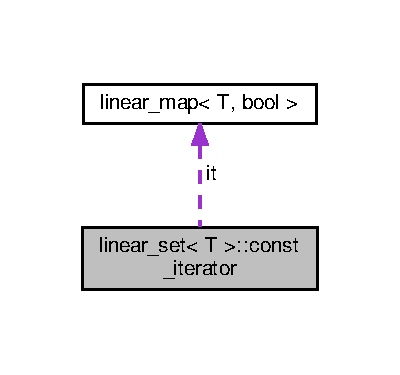
\includegraphics[width=192pt]{classlinear__set_1_1const__iterator__coll__graph}
\end{center}
\end{figure}
\subsection*{Tipos públicos}
\begin{DoxyCompactItemize}
\item 
\hypertarget{classlinear__set_1_1const__iterator_aeeb487937ec4d79cb6a1a08e73ac1f99}{using {\bfseries value\-\_\-type} = linear\-\_\-set\-::value\-\_\-type}\label{classlinear__set_1_1const__iterator_aeeb487937ec4d79cb6a1a08e73ac1f99}

\item 
\hypertarget{classlinear__set_1_1const__iterator_aa1f033d1d6817bba87a8a56db432f2e0}{using {\bfseries iterator\-\_\-category} = std\-::forward\-\_\-iterator\-\_\-tag}\label{classlinear__set_1_1const__iterator_aa1f033d1d6817bba87a8a56db432f2e0}

\item 
\hypertarget{classlinear__set_1_1const__iterator_a081f0692047d474e34e1ce924d3485ee}{using {\bfseries reference} = value\-\_\-type \&}\label{classlinear__set_1_1const__iterator_a081f0692047d474e34e1ce924d3485ee}

\item 
\hypertarget{classlinear__set_1_1const__iterator_acdc3e59c21faf9becf4c4dcf4ca1bef2}{using {\bfseries pointer} = value\-\_\-type $\ast$}\label{classlinear__set_1_1const__iterator_acdc3e59c21faf9becf4c4dcf4ca1bef2}

\item 
\hypertarget{classlinear__set_1_1const__iterator_ab68189d3b549fd08aea83d540cb7a1b0}{using {\bfseries difference\-\_\-type} = std\-::ptrdiff\-\_\-t}\label{classlinear__set_1_1const__iterator_ab68189d3b549fd08aea83d540cb7a1b0}

\end{DoxyCompactItemize}
\subsection*{Métodos públicos}
\begin{DoxyCompactItemize}
\item 
\hyperlink{classlinear__set_1_1const__iterator_a14ea693ec9b2c14b9d0e4570718236cc}{const\-\_\-iterator} (const typename \hyperlink{classlinear__set}{linear\-\_\-set}$<$ T $>$\-::\hyperlink{classlinear__set_1_1const__iterator}{const\-\_\-iterator} \&)
\begin{DoxyCompactList}\small\item\em Constructor por copia del iterador. \end{DoxyCompactList}\item 
\hyperlink{classlinear__set_1_1const__iterator_af7541fcff16bc3f8b4aaa9cbfc6f4a08}{const\-\_\-iterator} (const typename \hyperlink{classlinear__set}{linear\-\_\-set}$<$ T $>$\-::\hyperlink{classlinear__set_1_1iterator}{iterator} \&)
\begin{DoxyCompactList}\small\item\em Conversión desde iterator. \end{DoxyCompactList}\item 
\hyperlink{classlinear__set_1_1const__iterator}{linear\-\_\-set\-::const\-\_\-iterator} \& \hyperlink{classlinear__set_1_1const__iterator_aae244f473a6bc213fb9cd16d5caf8b08}{operator++} ()
\begin{DoxyCompactList}\small\item\em Avanza el iterador una posición. \end{DoxyCompactList}\item 
const value\-\_\-type \& \hyperlink{classlinear__set_1_1const__iterator_a1b5ae6a04aa1932ba64d4db211f90148}{operator$\ast$} () const 
\begin{DoxyCompactList}\small\item\em Desreferencia el puntero. \end{DoxyCompactList}\item 
const value\-\_\-type $\ast$ \hyperlink{classlinear__set_1_1const__iterator_ae87d9a0975fc0204f67ae31cbc53cb99}{operator-\/$>$} () const 
\begin{DoxyCompactList}\small\item\em Operador flechita. \end{DoxyCompactList}\item 
bool \hyperlink{classlinear__set_1_1const__iterator_a8b4807ed9a81180aca7855bb1fca935c}{operator==} (const \hyperlink{classlinear__set}{linear\-\_\-set}$<$ T $>$\-::\hyperlink{classlinear__set_1_1const__iterator}{const\-\_\-iterator} \&other) const 
\begin{DoxyCompactList}\small\item\em Comparación entre iteradores. \end{DoxyCompactList}\item 
bool \hyperlink{classlinear__set_1_1const__iterator_aaf284dd1decbd51ca0afedb3093da2a7}{operator!=} (const \hyperlink{classlinear__set}{linear\-\_\-set}$<$ T $>$\-::\hyperlink{classlinear__set_1_1const__iterator}{const\-\_\-iterator} \&other) const 
\begin{DoxyCompactList}\small\item\em Comparación entre iteradores. \end{DoxyCompactList}\end{DoxyCompactItemize}
\subsection*{Métodos privados}
\begin{DoxyCompactItemize}
\item 
\hypertarget{classlinear__set_1_1const__iterator_a14bd9ad8205de2c6fab3d8504253ee78}{\hyperlink{classlinear__set_1_1const__iterator_a14bd9ad8205de2c6fab3d8504253ee78}{const\-\_\-iterator} (const typename \hyperlink{classlinear__map}{linear\-\_\-map}$<$ T, bool $>$\-::\hyperlink{classlinear__set_1_1const__iterator}{const\-\_\-iterator} \&)}\label{classlinear__set_1_1const__iterator_a14bd9ad8205de2c6fab3d8504253ee78}

\begin{DoxyCompactList}\small\item\em Constructor del iterador a partir de un iterador interno. \end{DoxyCompactList}\end{DoxyCompactItemize}
\subsection*{Atributos privados}
\begin{DoxyCompactItemize}
\item 
\hypertarget{classlinear__set_1_1const__iterator_a16ef6914efccf16bfcb659df265244f8}{\hyperlink{classlinear__map}{linear\-\_\-map}$<$ T, bool $>$\\*
\-::\hyperlink{classlinear__set_1_1const__iterator}{const\-\_\-iterator} {\bfseries it}}\label{classlinear__set_1_1const__iterator_a16ef6914efccf16bfcb659df265244f8}

\end{DoxyCompactItemize}
\subsection*{Amigas}
\begin{DoxyCompactItemize}
\item 
\hypertarget{classlinear__set_1_1const__iterator_a534ce5acb60190eb00d1f44365fa38b5}{class {\bfseries linear\-\_\-set$<$ T $>$}}\label{classlinear__set_1_1const__iterator_a534ce5acb60190eb00d1f44365fa38b5}

\end{DoxyCompactItemize}


\subsection{Documentación del constructor y destructor}
\hypertarget{classlinear__set_1_1const__iterator_a14ea693ec9b2c14b9d0e4570718236cc}{\index{linear\-\_\-set\-::const\-\_\-iterator@{linear\-\_\-set\-::const\-\_\-iterator}!const\-\_\-iterator@{const\-\_\-iterator}}
\index{const\-\_\-iterator@{const\-\_\-iterator}!linear_set::const_iterator@{linear\-\_\-set\-::const\-\_\-iterator}}
\subsubsection[{const\-\_\-iterator}]{\setlength{\rightskip}{0pt plus 5cm}template$<$typename T$>$ {\bf linear\-\_\-set}$<$ T $>$\-::const\-\_\-iterator\-::const\-\_\-iterator (
\begin{DoxyParamCaption}
\item[{const typename {\bf linear\-\_\-set}$<$ T $>$\-::{\bf const\-\_\-iterator} \&}]{}
\end{DoxyParamCaption}
)}}\label{classlinear__set_1_1const__iterator_a14ea693ec9b2c14b9d0e4570718236cc}


Constructor por copia del iterador. 


\begin{DoxyDescription}
\item[Complejidad Temporal]$O$(1)
\end{DoxyDescription}\hypertarget{classlinear__set_1_1const__iterator_af7541fcff16bc3f8b4aaa9cbfc6f4a08}{\index{linear\-\_\-set\-::const\-\_\-iterator@{linear\-\_\-set\-::const\-\_\-iterator}!const\-\_\-iterator@{const\-\_\-iterator}}
\index{const\-\_\-iterator@{const\-\_\-iterator}!linear_set::const_iterator@{linear\-\_\-set\-::const\-\_\-iterator}}
\subsubsection[{const\-\_\-iterator}]{\setlength{\rightskip}{0pt plus 5cm}template$<$typename T$>$ {\bf linear\-\_\-set}$<$ T $>$\-::const\-\_\-iterator\-::const\-\_\-iterator (
\begin{DoxyParamCaption}
\item[{const typename {\bf linear\-\_\-set}$<$ T $>$\-::{\bf iterator} \&}]{}
\end{DoxyParamCaption}
)}}\label{classlinear__set_1_1const__iterator_af7541fcff16bc3f8b4aaa9cbfc6f4a08}


Conversión desde iterator. 


\begin{DoxyDescription}
\item[Complejidad Temporal]$O$(1)
\end{DoxyDescription}

\subsection{Documentación de las funciones miembro}
\hypertarget{classlinear__set_1_1const__iterator_aaf284dd1decbd51ca0afedb3093da2a7}{\index{linear\-\_\-set\-::const\-\_\-iterator@{linear\-\_\-set\-::const\-\_\-iterator}!operator!=@{operator!=}}
\index{operator!=@{operator!=}!linear_set::const_iterator@{linear\-\_\-set\-::const\-\_\-iterator}}
\subsubsection[{operator!=}]{\setlength{\rightskip}{0pt plus 5cm}template$<$typename T$>$ bool {\bf linear\-\_\-set}$<$ T $>$\-::const\-\_\-iterator\-::operator!= (
\begin{DoxyParamCaption}
\item[{const {\bf linear\-\_\-set}$<$ T $>$\-::{\bf const\-\_\-iterator} \&}]{other}
\end{DoxyParamCaption}
) const}}\label{classlinear__set_1_1const__iterator_aaf284dd1decbd51ca0afedb3093da2a7}


Comparación entre iteradores. 

\begin{DoxyPrecond}{Precondición}
ambos iteradores refieren a la misma colección 
\end{DoxyPrecond}
\begin{DoxyPostcond}{Postcondición}
true sii los iteradores no apuntan al mismo elemento
\end{DoxyPostcond}

\begin{DoxyDescription}
\item[Complejidad Temporal]$O$(1)
\end{DoxyDescription}\hypertarget{classlinear__set_1_1const__iterator_a1b5ae6a04aa1932ba64d4db211f90148}{\index{linear\-\_\-set\-::const\-\_\-iterator@{linear\-\_\-set\-::const\-\_\-iterator}!operator$\ast$@{operator$\ast$}}
\index{operator$\ast$@{operator$\ast$}!linear_set::const_iterator@{linear\-\_\-set\-::const\-\_\-iterator}}
\subsubsection[{operator$\ast$}]{\setlength{\rightskip}{0pt plus 5cm}template$<$typename T$>$ const {\bf linear\-\_\-set}$<$ T $>$\-::const\-\_\-iterator\-::value\-\_\-type \& {\bf linear\-\_\-set}$<$ T $>$\-::const\-\_\-iterator\-::operator$\ast$ (
\begin{DoxyParamCaption}
{}
\end{DoxyParamCaption}
) const}}\label{classlinear__set_1_1const__iterator_a1b5ae6a04aa1932ba64d4db211f90148}


Desreferencia el puntero. 

El valor devuelto tiene aliasing dentro de la colección.

\begin{DoxyPrecond}{Precondición}
El iterador no debe estar en la posición pasando-\/el-\/último. 
\end{DoxyPrecond}
\begin{DoxyPostcond}{Postcondición}
El valor resultado es una referencia constante al valor apuntado.
\end{DoxyPostcond}

\begin{DoxyDescription}
\item[Complejidad Temporal]$O$(1)
\end{DoxyDescription}\hypertarget{classlinear__set_1_1const__iterator_aae244f473a6bc213fb9cd16d5caf8b08}{\index{linear\-\_\-set\-::const\-\_\-iterator@{linear\-\_\-set\-::const\-\_\-iterator}!operator++@{operator++}}
\index{operator++@{operator++}!linear_set::const_iterator@{linear\-\_\-set\-::const\-\_\-iterator}}
\subsubsection[{operator++}]{\setlength{\rightskip}{0pt plus 5cm}template$<$typename T$>$ {\bf linear\-\_\-set}$<$ T $>$\-::{\bf const\-\_\-iterator} \& {\bf linear\-\_\-set}$<$ T $>$\-::const\-\_\-iterator\-::operator++ (
\begin{DoxyParamCaption}
{}
\end{DoxyParamCaption}
)}}\label{classlinear__set_1_1const__iterator_aae244f473a6bc213fb9cd16d5caf8b08}


Avanza el iterador una posición. 

\begin{DoxyPrecond}{Precondición}
El iterador no debe estar en la posición pasando-\/el-\/último. 
\end{DoxyPrecond}
\begin{DoxyPostcond}{Postcondición}
{\bfseries res} es una referencia a {\bfseries this}. {\bfseries this} apunta a la posición siguiente.
\end{DoxyPostcond}

\begin{DoxyDescription}
\item[Complejidad Temporal]$O$(1)
\end{DoxyDescription}\hypertarget{classlinear__set_1_1const__iterator_ae87d9a0975fc0204f67ae31cbc53cb99}{\index{linear\-\_\-set\-::const\-\_\-iterator@{linear\-\_\-set\-::const\-\_\-iterator}!operator-\/$>$@{operator-\/$>$}}
\index{operator-\/$>$@{operator-\/$>$}!linear_set::const_iterator@{linear\-\_\-set\-::const\-\_\-iterator}}
\subsubsection[{operator-\/$>$}]{\setlength{\rightskip}{0pt plus 5cm}template$<$typename T$>$ const {\bf linear\-\_\-set}$<$ T $>$\-::const\-\_\-iterator\-::value\-\_\-type $\ast$ {\bf linear\-\_\-set}$<$ T $>$\-::const\-\_\-iterator\-::operator-\/$>$ (
\begin{DoxyParamCaption}
{}
\end{DoxyParamCaption}
) const}}\label{classlinear__set_1_1const__iterator_ae87d9a0975fc0204f67ae31cbc53cb99}


Operador flechita. 

El valor devuelvo tiene aliasing dentro de la colección.

\begin{DoxyPrecond}{Precondición}
El iterador no debe estar en la posición pasando-\/el-\/último. 
\end{DoxyPrecond}
\begin{DoxyPostcond}{Postcondición}
El valor resultado es un puntero al valor apuntado.
\end{DoxyPostcond}

\begin{DoxyDescription}
\item[Complejidad Temporal]$O$(1)
\end{DoxyDescription}\hypertarget{classlinear__set_1_1const__iterator_a8b4807ed9a81180aca7855bb1fca935c}{\index{linear\-\_\-set\-::const\-\_\-iterator@{linear\-\_\-set\-::const\-\_\-iterator}!operator==@{operator==}}
\index{operator==@{operator==}!linear_set::const_iterator@{linear\-\_\-set\-::const\-\_\-iterator}}
\subsubsection[{operator==}]{\setlength{\rightskip}{0pt plus 5cm}template$<$typename T$>$ bool {\bf linear\-\_\-set}$<$ T $>$\-::const\-\_\-iterator\-::operator== (
\begin{DoxyParamCaption}
\item[{const {\bf linear\-\_\-set}$<$ T $>$\-::{\bf const\-\_\-iterator} \&}]{other}
\end{DoxyParamCaption}
) const}}\label{classlinear__set_1_1const__iterator_a8b4807ed9a81180aca7855bb1fca935c}


Comparación entre iteradores. 

\begin{DoxyPrecond}{Precondición}
ambos iteradores refieren a la misma colección 
\end{DoxyPrecond}
\begin{DoxyPostcond}{Postcondición}
true sii los iteradores apuntan al mismo elemento
\end{DoxyPostcond}

\begin{DoxyDescription}
\item[Complejidad Temporal]$O$(1)
\end{DoxyDescription}

La documentación para esta clase fue generada a partir del siguiente fichero\-:\begin{DoxyCompactItemize}
\item 
src/linear\-\_\-set\-\_\-iterators.\-h\end{DoxyCompactItemize}

\hypertarget{classstring__map_1_1const__iterator}{\section{Referencia de la Clase string\-\_\-map$<$ T $>$\-:\-:const\-\_\-iterator}
\label{classstring__map_1_1const__iterator}\index{string\-\_\-map$<$ T $>$\-::const\-\_\-iterator@{string\-\_\-map$<$ T $>$\-::const\-\_\-iterator}}
}


Diagrama de colaboración para string\-\_\-map$<$ T $>$\-:\-:const\-\_\-iterator\-:
\nopagebreak
\begin{figure}[H]
\begin{center}
\leavevmode
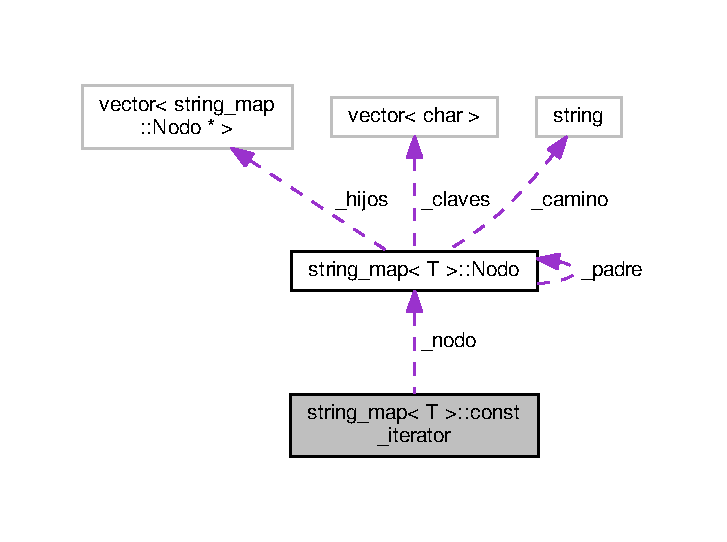
\includegraphics[width=349pt]{classstring__map_1_1const__iterator__coll__graph}
\end{center}
\end{figure}
\subsection*{Tipos públicos}
\begin{DoxyCompactItemize}
\item 
\hypertarget{classstring__map_1_1const__iterator_aca26e411b4326a7c43af783a3256cdbd}{using {\bfseries value\-\_\-type} = \hyperlink{classstring__map}{string\-\_\-map}$<$ T $>$\-::value\-\_\-type}\label{classstring__map_1_1const__iterator_aca26e411b4326a7c43af783a3256cdbd}

\item 
\hypertarget{classstring__map_1_1const__iterator_a9040c24531a149fbb6d4718786155234}{using {\bfseries reference} = value\-\_\-type \&}\label{classstring__map_1_1const__iterator_a9040c24531a149fbb6d4718786155234}

\item 
\hypertarget{classstring__map_1_1const__iterator_a1b3a30bbc774ac416d551b2c023cf6d7}{using {\bfseries pointer} = value\-\_\-type $\ast$}\label{classstring__map_1_1const__iterator_a1b3a30bbc774ac416d551b2c023cf6d7}

\end{DoxyCompactItemize}
\subsection*{Métodos públicos}
\begin{DoxyCompactItemize}
\item 
\hyperlink{classstring__map_1_1const__iterator_a34833166008a59e0d3b4758ba1154a9f}{const\-\_\-iterator} (const typename \hyperlink{classstring__map}{string\-\_\-map}$<$ T $>$\-::\hyperlink{classstring__map_1_1const__iterator}{const\-\_\-iterator} \&)
\begin{DoxyCompactList}\small\item\em Constructor por copia del iterador. \end{DoxyCompactList}\item 
\hypertarget{classstring__map_1_1const__iterator_acc80ad43b0d553e73a42c286f2f1edae}{{\bfseries const\-\_\-iterator} (const typename \hyperlink{classstring__map}{string\-\_\-map}$<$ T $>$\-::\hyperlink{structstring__map_1_1Nodo}{Nodo} $\ast$)}\label{classstring__map_1_1const__iterator_acc80ad43b0d553e73a42c286f2f1edae}

\item 
\hyperlink{classstring__map_1_1const__iterator_a615c996037b07d56db8de0f7775b1a57}{const\-\_\-iterator} (const typename \hyperlink{classstring__map}{string\-\_\-map}$<$ T $>$\-::\hyperlink{classstring__map_1_1iterator}{iterator} \&)
\begin{DoxyCompactList}\small\item\em Conversión desde iterator. \end{DoxyCompactList}\item 
\hyperlink{classstring__map_1_1const__iterator}{string\-\_\-map\-::const\-\_\-iterator} \& \hyperlink{classstring__map_1_1const__iterator_aba282a526ddb0685bd1433998484181e}{operator++} ()
\begin{DoxyCompactList}\small\item\em Avanza el iterador una posición. \end{DoxyCompactList}\item 
const value\-\_\-type \& \hyperlink{classstring__map_1_1const__iterator_a0efad597b0ffe1a1db9fe46be5802ef5}{operator$\ast$} () const 
\begin{DoxyCompactList}\small\item\em Desreferencia el puntero. \end{DoxyCompactList}\item 
const value\-\_\-type $\ast$ \hyperlink{classstring__map_1_1const__iterator_aa892ecb777d31558fca1933613d6ea9d}{operator-\/$>$} () const 
\begin{DoxyCompactList}\small\item\em Operador flechita. \end{DoxyCompactList}\item 
bool \hyperlink{classstring__map_1_1const__iterator_adca0fb340d1da380d7eb2ace2dd4f1d0}{operator==} (const \hyperlink{classstring__map}{string\-\_\-map}$<$ T $>$\-::\hyperlink{classstring__map_1_1const__iterator}{const\-\_\-iterator} \&other) const 
\begin{DoxyCompactList}\small\item\em Comparación entre iteradores. \end{DoxyCompactList}\item 
bool \hyperlink{classstring__map_1_1const__iterator_a80a030933f7794456a8cb6e79db96d23}{operator!=} (const \hyperlink{classstring__map}{string\-\_\-map}$<$ T $>$\-::\hyperlink{classstring__map_1_1const__iterator}{const\-\_\-iterator} \&other) const 
\begin{DoxyCompactList}\small\item\em Comparación entre iteradores. \end{DoxyCompactList}\end{DoxyCompactItemize}
\subsection*{Métodos privados}
\begin{DoxyCompactItemize}
\item 
\hypertarget{classstring__map_1_1const__iterator_a9e7b24c524e269c5e910615e77548f01}{\hyperlink{classstring__map_1_1const__iterator_a9e7b24c524e269c5e910615e77548f01}{const\-\_\-iterator} (\hyperlink{structstring__map_1_1Nodo}{Nodo} $\ast$n)}\label{classstring__map_1_1const__iterator_a9e7b24c524e269c5e910615e77548f01}

\begin{DoxyCompactList}\small\item\em El iterador es puntero a \hyperlink{structstring__map_1_1Nodo}{Nodo}. \end{DoxyCompactList}\end{DoxyCompactItemize}
\subsection*{Atributos privados}
\begin{DoxyCompactItemize}
\item 
\hypertarget{classstring__map_1_1const__iterator_a92196635e36d6acff25921951cf4a51a}{\hyperlink{structstring__map_1_1Nodo}{Nodo} $\ast$ {\bfseries \-\_\-nodo}}\label{classstring__map_1_1const__iterator_a92196635e36d6acff25921951cf4a51a}

\end{DoxyCompactItemize}
\subsection*{Amigas}
\begin{DoxyCompactItemize}
\item 
\hypertarget{classstring__map_1_1const__iterator_ad0a70c0d4333f3435a234a4682421708}{class {\bfseries string\-\_\-map$<$ T $>$}}\label{classstring__map_1_1const__iterator_ad0a70c0d4333f3435a234a4682421708}

\end{DoxyCompactItemize}


\subsection{Documentación del constructor y destructor}
\hypertarget{classstring__map_1_1const__iterator_a34833166008a59e0d3b4758ba1154a9f}{\index{string\-\_\-map\-::const\-\_\-iterator@{string\-\_\-map\-::const\-\_\-iterator}!const\-\_\-iterator@{const\-\_\-iterator}}
\index{const\-\_\-iterator@{const\-\_\-iterator}!string_map::const_iterator@{string\-\_\-map\-::const\-\_\-iterator}}
\subsubsection[{const\-\_\-iterator}]{\setlength{\rightskip}{0pt plus 5cm}template$<$typename T$>$ {\bf string\-\_\-map}$<$ T $>$\-::const\-\_\-iterator\-::const\-\_\-iterator (
\begin{DoxyParamCaption}
\item[{const typename {\bf string\-\_\-map}$<$ T $>$\-::{\bf const\-\_\-iterator} \&}]{}
\end{DoxyParamCaption}
)}}\label{classstring__map_1_1const__iterator_a34833166008a59e0d3b4758ba1154a9f}


Constructor por copia del iterador. 


\begin{DoxyDescription}
\item[Complejidad Temporal]$O$(1)
\end{DoxyDescription}\hypertarget{classstring__map_1_1const__iterator_a615c996037b07d56db8de0f7775b1a57}{\index{string\-\_\-map\-::const\-\_\-iterator@{string\-\_\-map\-::const\-\_\-iterator}!const\-\_\-iterator@{const\-\_\-iterator}}
\index{const\-\_\-iterator@{const\-\_\-iterator}!string_map::const_iterator@{string\-\_\-map\-::const\-\_\-iterator}}
\subsubsection[{const\-\_\-iterator}]{\setlength{\rightskip}{0pt plus 5cm}template$<$typename T$>$ {\bf string\-\_\-map}$<$ T $>$\-::const\-\_\-iterator\-::const\-\_\-iterator (
\begin{DoxyParamCaption}
\item[{const typename {\bf string\-\_\-map}$<$ T $>$\-::{\bf iterator} \&}]{}
\end{DoxyParamCaption}
)}}\label{classstring__map_1_1const__iterator_a615c996037b07d56db8de0f7775b1a57}


Conversión desde iterator. 


\begin{DoxyDescription}
\item[Complejidad Temporal]$O$(1)
\end{DoxyDescription}

\subsection{Documentación de las funciones miembro}
\hypertarget{classstring__map_1_1const__iterator_a80a030933f7794456a8cb6e79db96d23}{\index{string\-\_\-map\-::const\-\_\-iterator@{string\-\_\-map\-::const\-\_\-iterator}!operator!=@{operator!=}}
\index{operator!=@{operator!=}!string_map::const_iterator@{string\-\_\-map\-::const\-\_\-iterator}}
\subsubsection[{operator!=}]{\setlength{\rightskip}{0pt plus 5cm}template$<$typename T$>$ bool {\bf string\-\_\-map}$<$ T $>$\-::const\-\_\-iterator\-::operator!= (
\begin{DoxyParamCaption}
\item[{const {\bf string\-\_\-map}$<$ T $>$\-::{\bf const\-\_\-iterator} \&}]{other}
\end{DoxyParamCaption}
) const}}\label{classstring__map_1_1const__iterator_a80a030933f7794456a8cb6e79db96d23}


Comparación entre iteradores. 

\begin{DoxyPrecond}{Precondición}
ambos iteradores refieren a la misma colección 
\end{DoxyPrecond}
\begin{DoxyPostcond}{Postcondición}
true sii los iteradores no apuntan al mismo elemento
\end{DoxyPostcond}

\begin{DoxyDescription}
\item[Complejidad Temporal]$O$(1)
\end{DoxyDescription}\hypertarget{classstring__map_1_1const__iterator_a0efad597b0ffe1a1db9fe46be5802ef5}{\index{string\-\_\-map\-::const\-\_\-iterator@{string\-\_\-map\-::const\-\_\-iterator}!operator$\ast$@{operator$\ast$}}
\index{operator$\ast$@{operator$\ast$}!string_map::const_iterator@{string\-\_\-map\-::const\-\_\-iterator}}
\subsubsection[{operator$\ast$}]{\setlength{\rightskip}{0pt plus 5cm}template$<$typename T$>$ const {\bf string\-\_\-map}$<$ T $>$\-::const\-\_\-iterator\-::value\-\_\-type \& {\bf string\-\_\-map}$<$ T $>$\-::const\-\_\-iterator\-::operator$\ast$ (
\begin{DoxyParamCaption}
{}
\end{DoxyParamCaption}
) const}}\label{classstring__map_1_1const__iterator_a0efad597b0ffe1a1db9fe46be5802ef5}


Desreferencia el puntero. 

El valor devuelto tiene aliasing dentro de la colección.

\begin{DoxyPrecond}{Precondición}
El iterador no debe estar en la posición pasando-\/el-\/último. 
\end{DoxyPrecond}
\begin{DoxyPostcond}{Postcondición}
El valor resultado es una referencia constante al valor apuntado.
\end{DoxyPostcond}

\begin{DoxyDescription}
\item[Complejidad Temporal]$O$(1)
\end{DoxyDescription}\hypertarget{classstring__map_1_1const__iterator_aba282a526ddb0685bd1433998484181e}{\index{string\-\_\-map\-::const\-\_\-iterator@{string\-\_\-map\-::const\-\_\-iterator}!operator++@{operator++}}
\index{operator++@{operator++}!string_map::const_iterator@{string\-\_\-map\-::const\-\_\-iterator}}
\subsubsection[{operator++}]{\setlength{\rightskip}{0pt plus 5cm}template$<$typename T$>$ {\bf string\-\_\-map}$<$ T $>$\-::{\bf const\-\_\-iterator} \& {\bf string\-\_\-map}$<$ T $>$\-::const\-\_\-iterator\-::operator++ (
\begin{DoxyParamCaption}
{}
\end{DoxyParamCaption}
)}}\label{classstring__map_1_1const__iterator_aba282a526ddb0685bd1433998484181e}


Avanza el iterador una posición. 

\begin{DoxyPrecond}{Precondición}
El iterador no debe estar en la posición pasando-\/el-\/último. 
\end{DoxyPrecond}
\begin{DoxyPostcond}{Postcondición}
{\bfseries res} es una referencia a {\bfseries this}. {\bfseries this} apunta a la posición siguiente.
\end{DoxyPostcond}

\begin{DoxyDescription}
\item[Complejidad Temporal]$O$(1)
\end{DoxyDescription}\hypertarget{classstring__map_1_1const__iterator_aa892ecb777d31558fca1933613d6ea9d}{\index{string\-\_\-map\-::const\-\_\-iterator@{string\-\_\-map\-::const\-\_\-iterator}!operator-\/$>$@{operator-\/$>$}}
\index{operator-\/$>$@{operator-\/$>$}!string_map::const_iterator@{string\-\_\-map\-::const\-\_\-iterator}}
\subsubsection[{operator-\/$>$}]{\setlength{\rightskip}{0pt plus 5cm}template$<$typename T$>$ const {\bf string\-\_\-map}$<$ T $>$\-::const\-\_\-iterator\-::value\-\_\-type $\ast$ {\bf string\-\_\-map}$<$ T $>$\-::const\-\_\-iterator\-::operator-\/$>$ (
\begin{DoxyParamCaption}
{}
\end{DoxyParamCaption}
) const}}\label{classstring__map_1_1const__iterator_aa892ecb777d31558fca1933613d6ea9d}


Operador flechita. 

El valor devuelvo tiene aliasing dentro de la colección.

\begin{DoxyPrecond}{Precondición}
El iterador no debe estar en la posición pasando-\/el-\/último. 
\end{DoxyPrecond}
\begin{DoxyPostcond}{Postcondición}
El valor resultado es un puntero al valor apuntado.
\end{DoxyPostcond}

\begin{DoxyDescription}
\item[Complejidad Temporal]$O$(1)
\end{DoxyDescription}\hypertarget{classstring__map_1_1const__iterator_adca0fb340d1da380d7eb2ace2dd4f1d0}{\index{string\-\_\-map\-::const\-\_\-iterator@{string\-\_\-map\-::const\-\_\-iterator}!operator==@{operator==}}
\index{operator==@{operator==}!string_map::const_iterator@{string\-\_\-map\-::const\-\_\-iterator}}
\subsubsection[{operator==}]{\setlength{\rightskip}{0pt plus 5cm}template$<$typename T$>$ bool {\bf string\-\_\-map}$<$ T $>$\-::const\-\_\-iterator\-::operator== (
\begin{DoxyParamCaption}
\item[{const {\bf string\-\_\-map}$<$ T $>$\-::{\bf const\-\_\-iterator} \&}]{other}
\end{DoxyParamCaption}
) const}}\label{classstring__map_1_1const__iterator_adca0fb340d1da380d7eb2ace2dd4f1d0}


Comparación entre iteradores. 

\begin{DoxyPrecond}{Precondición}
ambos iteradores refieren a la misma colección 
\end{DoxyPrecond}
\begin{DoxyPostcond}{Postcondición}
true sii los iteradores apuntan al mismo elemento
\end{DoxyPostcond}

\begin{DoxyDescription}
\item[Complejidad Temporal]$O$(1)
\end{DoxyDescription}

La documentación para esta clase fue generada a partir del siguiente fichero\-:\begin{DoxyCompactItemize}
\item 
src/string\-\_\-map\-\_\-iterators.\-h\end{DoxyCompactItemize}

\hypertarget{classDato}{\section{Referencia de la Clase Dato}
\label{classDato}\index{Dato@{Dato}}
}


Representa un \hyperlink{classDato}{Dato} de una Base de Datos.  




{\ttfamily \#include $<$Dato.\-h$>$}



Diagrama de colaboración para Dato\-:
\nopagebreak
\begin{figure}[H]
\begin{center}
\leavevmode
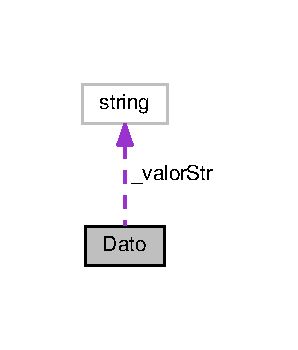
\includegraphics[width=143pt]{classDato__coll__graph}
\end{center}
\end{figure}
\subsection*{Métodos públicos}
\begin{DoxyCompactItemize}
\item 
\hyperlink{classDato_a008b1dadda8ec2557cc88886da907523}{Dato} ()
\begin{DoxyCompactList}\small\item\em Constructor sin parametros para un dato trivial. \end{DoxyCompactList}\item 
\hyperlink{classDato_aeb115751623b17f5cc61199c45dd6fb4}{Dato} (int \hyperlink{classDato_a417fa8d0766c8ac1221c553b0f31ba93}{valor\-Nat})
\begin{DoxyCompactList}\small\item\em Constructor de dato con valor nat. \end{DoxyCompactList}\item 
\hyperlink{classDato_a3b8e8b3472eee6374487378e865e3428}{Dato} (const string \&\hyperlink{classDato_ac1ece791ad4cc21764a89ffac254add8}{valor\-Str})
\begin{DoxyCompactList}\small\item\em Constructor de dato con valor string. \end{DoxyCompactList}\item 
bool \hyperlink{classDato_a815f643cd190da9ddf25e1c91d0eb7fa}{es\-Nat} () const 
\begin{DoxyCompactList}\small\item\em True si el dato es de tipo nat. \end{DoxyCompactList}\item 
bool \hyperlink{classDato_a25bc3327023f6d84729d64d61800937b}{es\-String} () const 
\begin{DoxyCompactList}\small\item\em True si el dato es de tipo string. \end{DoxyCompactList}\item 
string \hyperlink{classDato_ac1ece791ad4cc21764a89ffac254add8}{valor\-Str} () const 
\begin{DoxyCompactList}\small\item\em El valor del dato. \end{DoxyCompactList}\item 
int \hyperlink{classDato_a417fa8d0766c8ac1221c553b0f31ba93}{valor\-Nat} () const 
\begin{DoxyCompactList}\small\item\em El valor del dato. \end{DoxyCompactList}\end{DoxyCompactItemize}
\subsection*{Atributos privados}
\begin{Indent}{\bf Representación}\par
{\em rep\-: dato $\to$ bool\par
rep(d) $\equiv$
\begin{DoxyItemize}
\item \-\_\-es\-Nat $\Rightarrow$ \-\_\-valor\-Str = \char`\"{}\char`\"{} $\lor$ $\lnot$ \-\_\-es\-Nat $\Rightarrow$ \-\_\-valor\-Nat = 0
\end{DoxyItemize}

abs\-: dato $\to$ \hyperlink{classDato}{Dato}\par
abs(d) $\equiv$ d' $|$
\begin{DoxyItemize}
\item Nat?(d') = d.\-\_\-es\-Nat $\land$
\item Nat?(d') $\Rightarrow$ valor\-Nat(d) = d.\-\_\-valor\-Nat $\land$
\item Nat?(d') $\Rightarrow$ valor\-Str(d) = d.\-\_\-valor\-Str 
\end{DoxyItemize}}\begin{DoxyCompactItemize}
\item 
\hypertarget{classDato_a117b034b0acbfb4b602ab5445855f3f1}{int \hyperlink{classDato_a117b034b0acbfb4b602ab5445855f3f1}{\-\_\-valor\-Nat}}\label{classDato_a117b034b0acbfb4b602ab5445855f3f1}

\begin{DoxyCompactList}\small\item\em Valor cuando el dato es nat. \end{DoxyCompactList}\item 
\hypertarget{classDato_a4abdad075253c04b649282227a01bbed}{string \hyperlink{classDato_a4abdad075253c04b649282227a01bbed}{\-\_\-valor\-Str}}\label{classDato_a4abdad075253c04b649282227a01bbed}

\begin{DoxyCompactList}\small\item\em Valor cuando el dato es nat. \end{DoxyCompactList}\item 
\hypertarget{classDato_a43a0578f47ccb55da86088491f862bf9}{bool \hyperlink{classDato_a43a0578f47ccb55da86088491f862bf9}{\-\_\-es\-Nat}}\label{classDato_a43a0578f47ccb55da86088491f862bf9}

\begin{DoxyCompactList}\small\item\em Define si el dato es nat. \end{DoxyCompactList}\end{DoxyCompactItemize}
\end{Indent}
\subsection*{Amigas}
\begin{DoxyCompactItemize}
\item 
\hypertarget{classDato_a394289679728bdcb20171c43449894c1}{bool \hyperlink{classDato_a394289679728bdcb20171c43449894c1}{operator$<$} (const \hyperlink{classDato}{Dato} \&, const \hyperlink{classDato}{Dato} \&)}\label{classDato_a394289679728bdcb20171c43449894c1}

\begin{DoxyCompactList}\small\item\em Comparador de datos. \end{DoxyCompactList}\end{DoxyCompactItemize}


\subsection{Descripción detallada}
Representa un \hyperlink{classDato}{Dato} de una Base de Datos. 

{\bfseries se explica con} T\-A\-D \hyperlink{classDato}{Dato} 

\subsection{Documentación del constructor y destructor}
\hypertarget{classDato_a008b1dadda8ec2557cc88886da907523}{\index{Dato@{Dato}!Dato@{Dato}}
\index{Dato@{Dato}!Dato@{Dato}}
\subsubsection[{Dato}]{\setlength{\rightskip}{0pt plus 5cm}Dato\-::\-Dato (
\begin{DoxyParamCaption}
{}
\end{DoxyParamCaption}
)}}\label{classDato_a008b1dadda8ec2557cc88886da907523}


Constructor sin parametros para un dato trivial. 

\begin{DoxyPrecond}{Precondición}
true 
\end{DoxyPrecond}
\begin{DoxyPostcond}{Postcondición}
true 
\begin{DoxyDescription}
\item[Complejidad Temporal]$O$(1)
\end{DoxyDescription}
\end{DoxyPostcond}
\hypertarget{classDato_aeb115751623b17f5cc61199c45dd6fb4}{\index{Dato@{Dato}!Dato@{Dato}}
\index{Dato@{Dato}!Dato@{Dato}}
\subsubsection[{Dato}]{\setlength{\rightskip}{0pt plus 5cm}Dato\-::\-Dato (
\begin{DoxyParamCaption}
\item[{int}]{valor\-Nat}
\end{DoxyParamCaption}
)}}\label{classDato_aeb115751623b17f5cc61199c45dd6fb4}


Constructor de dato con valor nat. 


\begin{DoxyParams}{Parámetros}
{\em valor\-Nat} & valor natural del dato\\
\hline
\end{DoxyParams}
\begin{DoxyPrecond}{Precondición}
true 
\end{DoxyPrecond}
\begin{DoxyPostcond}{Postcondición}
{\bfseries res} $=_{\rm obs}$ dato\-Nat(valor\-Nat) 
\begin{DoxyDescription}
\item[Complejidad Temporal]$O$(1)
\end{DoxyDescription}
\end{DoxyPostcond}
\hypertarget{classDato_a3b8e8b3472eee6374487378e865e3428}{\index{Dato@{Dato}!Dato@{Dato}}
\index{Dato@{Dato}!Dato@{Dato}}
\subsubsection[{Dato}]{\setlength{\rightskip}{0pt plus 5cm}Dato\-::\-Dato (
\begin{DoxyParamCaption}
\item[{const string \&}]{valor\-Str}
\end{DoxyParamCaption}
)}}\label{classDato_a3b8e8b3472eee6374487378e865e3428}


Constructor de dato con valor string. 


\begin{DoxyParams}{Parámetros}
{\em valor\-Str} & valor string del dato\\
\hline
\end{DoxyParams}
\begin{DoxyPrecond}{Precondición}
true 
\end{DoxyPrecond}
\begin{DoxyPostcond}{Postcondición}
{\bfseries res} $=_{\rm obs}$ dato\-Str(valor\-Str) 
\begin{DoxyDescription}
\item[Complejidad Temporal]$O$(1)
\end{DoxyDescription}
\end{DoxyPostcond}


\subsection{Documentación de las funciones miembro}
\hypertarget{classDato_a815f643cd190da9ddf25e1c91d0eb7fa}{\index{Dato@{Dato}!es\-Nat@{es\-Nat}}
\index{es\-Nat@{es\-Nat}!Dato@{Dato}}
\subsubsection[{es\-Nat}]{\setlength{\rightskip}{0pt plus 5cm}bool Dato\-::es\-Nat (
\begin{DoxyParamCaption}
{}
\end{DoxyParamCaption}
) const}}\label{classDato_a815f643cd190da9ddf25e1c91d0eb7fa}


True si el dato es de tipo nat. 

\begin{DoxyPrecond}{Precondición}
true 
\end{DoxyPrecond}
\begin{DoxyPostcond}{Postcondición}
{\bfseries res} $=_{\rm obs}$ Nat?({\bfseries this}) 
\begin{DoxyDescription}
\item[Complejidad Temporal]$O$(1)
\end{DoxyDescription}
\end{DoxyPostcond}
\hypertarget{classDato_a25bc3327023f6d84729d64d61800937b}{\index{Dato@{Dato}!es\-String@{es\-String}}
\index{es\-String@{es\-String}!Dato@{Dato}}
\subsubsection[{es\-String}]{\setlength{\rightskip}{0pt plus 5cm}bool Dato\-::es\-String (
\begin{DoxyParamCaption}
{}
\end{DoxyParamCaption}
) const}}\label{classDato_a25bc3327023f6d84729d64d61800937b}


True si el dato es de tipo string. 

\begin{DoxyPrecond}{Precondición}
true 
\end{DoxyPrecond}
\begin{DoxyPostcond}{Postcondición}
{\bfseries res} $=_{\rm obs}$ String?({\bfseries this}) 
\begin{DoxyDescription}
\item[Complejidad Temporal]$O$(1)
\end{DoxyDescription}
\end{DoxyPostcond}
\hypertarget{classDato_a417fa8d0766c8ac1221c553b0f31ba93}{\index{Dato@{Dato}!valor\-Nat@{valor\-Nat}}
\index{valor\-Nat@{valor\-Nat}!Dato@{Dato}}
\subsubsection[{valor\-Nat}]{\setlength{\rightskip}{0pt plus 5cm}int Dato\-::valor\-Nat (
\begin{DoxyParamCaption}
{}
\end{DoxyParamCaption}
) const}}\label{classDato_a417fa8d0766c8ac1221c553b0f31ba93}


El valor del dato. 

Devuelve el valor por copia.

\begin{DoxyPrecond}{Precondición}
Nat?({\bfseries this}) 
\end{DoxyPrecond}
\begin{DoxyPostcond}{Postcondición}
{\bfseries res} $=_{\rm obs}$ valor\-Nat({\bfseries this}) 
\begin{DoxyDescription}
\item[Complejidad Temporal]$O$(1)
\end{DoxyDescription}
\end{DoxyPostcond}
\hypertarget{classDato_ac1ece791ad4cc21764a89ffac254add8}{\index{Dato@{Dato}!valor\-Str@{valor\-Str}}
\index{valor\-Str@{valor\-Str}!Dato@{Dato}}
\subsubsection[{valor\-Str}]{\setlength{\rightskip}{0pt plus 5cm}string Dato\-::valor\-Str (
\begin{DoxyParamCaption}
{}
\end{DoxyParamCaption}
) const}}\label{classDato_ac1ece791ad4cc21764a89ffac254add8}


El valor del dato. 

Devuelve el valor por copia.

\begin{DoxyPrecond}{Precondición}
String?({\bfseries this}) 
\end{DoxyPrecond}
\begin{DoxyPostcond}{Postcondición}
{\bfseries res} $=_{\rm obs}$ valor\-Str({\bfseries this}) 
\begin{DoxyDescription}
\item[Complejidad Temporal]$O$(1)
\end{DoxyDescription}
\end{DoxyPostcond}


La documentación para esta clase fue generada a partir de los siguientes ficheros\-:\begin{DoxyCompactItemize}
\item 
src/Dato.\-h\item 
src/Dato.\-cpp\end{DoxyCompactItemize}

\hypertarget{classlinear__set_1_1iterator}{\section{Referencia de la Clase linear\-\_\-set$<$ T $>$\-:\-:iterator}
\label{classlinear__set_1_1iterator}\index{linear\-\_\-set$<$ T $>$\-::iterator@{linear\-\_\-set$<$ T $>$\-::iterator}}
}


Diagrama de colaboración para linear\-\_\-set$<$ T $>$\-:\-:iterator\-:
\nopagebreak
\begin{figure}[H]
\begin{center}
\leavevmode
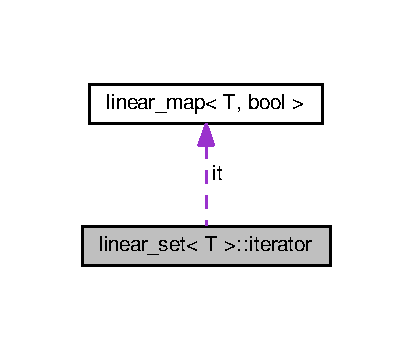
\includegraphics[width=198pt]{classlinear__set_1_1iterator__coll__graph}
\end{center}
\end{figure}
\subsection*{Tipos públicos}
\begin{DoxyCompactItemize}
\item 
\hypertarget{classlinear__set_1_1iterator_adc428ae224f2e66cded571df340b814e}{using {\bfseries value\-\_\-type} = const linear\-\_\-set\-::value\-\_\-type}\label{classlinear__set_1_1iterator_adc428ae224f2e66cded571df340b814e}

\item 
\hypertarget{classlinear__set_1_1iterator_ac70b54cbde97e1a59bc002979633aa41}{using {\bfseries iterator\-\_\-category} = std\-::forward\-\_\-iterator\-\_\-tag}\label{classlinear__set_1_1iterator_ac70b54cbde97e1a59bc002979633aa41}

\item 
\hypertarget{classlinear__set_1_1iterator_a1394508ada8427ad0b5764794ea59473}{using {\bfseries reference} = value\-\_\-type \&}\label{classlinear__set_1_1iterator_a1394508ada8427ad0b5764794ea59473}

\item 
\hypertarget{classlinear__set_1_1iterator_a4334a22789e11ff18a1b31982a20f944}{using {\bfseries pointer} = value\-\_\-type $\ast$}\label{classlinear__set_1_1iterator_a4334a22789e11ff18a1b31982a20f944}

\item 
\hypertarget{classlinear__set_1_1iterator_aca6addc2ad85f15d075c225c4ad3a085}{using {\bfseries difference\-\_\-type} = std\-::ptrdiff\-\_\-t}\label{classlinear__set_1_1iterator_aca6addc2ad85f15d075c225c4ad3a085}

\end{DoxyCompactItemize}
\subsection*{Métodos públicos}
\begin{DoxyCompactItemize}
\item 
\hyperlink{classlinear__set_1_1iterator_ab60c745272218eee7323209f4f115fbd}{iterator} (const typename \hyperlink{classlinear__set}{linear\-\_\-set}$<$ T $>$\-::\hyperlink{classlinear__set_1_1iterator}{iterator} \&)
\begin{DoxyCompactList}\small\item\em Constructor por copia del iterador. \end{DoxyCompactList}\item 
\hyperlink{classlinear__set_1_1iterator}{linear\-\_\-set\-::iterator} \& \hyperlink{classlinear__set_1_1iterator_a5520c75db974b7f2f61d677bc5ae4d0d}{operator++} ()
\begin{DoxyCompactList}\small\item\em Avanza el iterador una posición. \end{DoxyCompactList}\item 
const value\-\_\-type \& \hyperlink{classlinear__set_1_1iterator_aaa433eb1d7edd4854cda8b27464f0e5f}{operator$\ast$} () const 
\begin{DoxyCompactList}\small\item\em Desreferencia el puntero. \end{DoxyCompactList}\item 
const value\-\_\-type $\ast$ \hyperlink{classlinear__set_1_1iterator_ac7245da07e968927586744ee582df638}{operator-\/$>$} () const 
\begin{DoxyCompactList}\small\item\em Operador flechita. \end{DoxyCompactList}\item 
bool \hyperlink{classlinear__set_1_1iterator_a1e80ff416da110a71b1944bc9f05ed12}{operator==} (const \hyperlink{classlinear__set}{linear\-\_\-set}$<$ T $>$\-::\hyperlink{classlinear__set_1_1iterator}{iterator} \&other) const 
\begin{DoxyCompactList}\small\item\em Comparación entre iteradores. \end{DoxyCompactList}\item 
bool \hyperlink{classlinear__set_1_1iterator_a5c6c1cf3f266116b12563effc6644711}{operator!=} (const \hyperlink{classlinear__set}{linear\-\_\-set}$<$ T $>$\-::\hyperlink{classlinear__set_1_1iterator}{iterator} \&other) const 
\begin{DoxyCompactList}\small\item\em Comparación entre iteradores. \end{DoxyCompactList}\end{DoxyCompactItemize}
\subsection*{Métodos privados}
\begin{DoxyCompactItemize}
\item 
\hypertarget{classlinear__set_1_1iterator_a6778932b66a53ffd0efc46d26a0710c3}{\hyperlink{classlinear__set_1_1iterator_a6778932b66a53ffd0efc46d26a0710c3}{iterator} (const typename \hyperlink{classlinear__map}{linear\-\_\-map}$<$ T, bool $>$\-::\hyperlink{classlinear__set_1_1iterator}{iterator} \&)}\label{classlinear__set_1_1iterator_a6778932b66a53ffd0efc46d26a0710c3}

\begin{DoxyCompactList}\small\item\em Constructor del iterador a partir de un iterador interno. \end{DoxyCompactList}\end{DoxyCompactItemize}
\subsection*{Atributos privados}
\begin{DoxyCompactItemize}
\item 
\hypertarget{classlinear__set_1_1iterator_ae79df8b590ffcf8cd07a4751f859e882}{\hyperlink{classlinear__map}{linear\-\_\-map}$<$ T, bool $>$\-::\hyperlink{classlinear__set_1_1iterator}{iterator} {\bfseries it}}\label{classlinear__set_1_1iterator_ae79df8b590ffcf8cd07a4751f859e882}

\end{DoxyCompactItemize}
\subsection*{Amigas}
\begin{DoxyCompactItemize}
\item 
\hypertarget{classlinear__set_1_1iterator_a534ce5acb60190eb00d1f44365fa38b5}{class {\bfseries linear\-\_\-set$<$ T $>$}}\label{classlinear__set_1_1iterator_a534ce5acb60190eb00d1f44365fa38b5}

\end{DoxyCompactItemize}


\subsection{Documentación del constructor y destructor}
\hypertarget{classlinear__set_1_1iterator_ab60c745272218eee7323209f4f115fbd}{\index{linear\-\_\-set\-::iterator@{linear\-\_\-set\-::iterator}!iterator@{iterator}}
\index{iterator@{iterator}!linear_set::iterator@{linear\-\_\-set\-::iterator}}
\subsubsection[{iterator}]{\setlength{\rightskip}{0pt plus 5cm}template$<$typename T$>$ {\bf linear\-\_\-set}$<$ T $>$\-::iterator\-::iterator (
\begin{DoxyParamCaption}
\item[{const typename {\bf linear\-\_\-set}$<$ T $>$\-::{\bf iterator} \&}]{}
\end{DoxyParamCaption}
)}}\label{classlinear__set_1_1iterator_ab60c745272218eee7323209f4f115fbd}


Constructor por copia del iterador. 


\begin{DoxyDescription}
\item[Complejidad Temporal]$O$(1)
\end{DoxyDescription}

\subsection{Documentación de las funciones miembro}
\hypertarget{classlinear__set_1_1iterator_a5c6c1cf3f266116b12563effc6644711}{\index{linear\-\_\-set\-::iterator@{linear\-\_\-set\-::iterator}!operator!=@{operator!=}}
\index{operator!=@{operator!=}!linear_set::iterator@{linear\-\_\-set\-::iterator}}
\subsubsection[{operator!=}]{\setlength{\rightskip}{0pt plus 5cm}template$<$typename T$>$ bool {\bf linear\-\_\-set}$<$ T $>$\-::iterator\-::operator!= (
\begin{DoxyParamCaption}
\item[{const {\bf linear\-\_\-set}$<$ T $>$\-::{\bf iterator} \&}]{other}
\end{DoxyParamCaption}
) const}}\label{classlinear__set_1_1iterator_a5c6c1cf3f266116b12563effc6644711}


Comparación entre iteradores. 

\begin{DoxyPrecond}{Precondición}
ambos iteradores refieren a la misma colección 
\end{DoxyPrecond}
\begin{DoxyPostcond}{Postcondición}
true sii los iteradores no apuntan al mismo elemento
\end{DoxyPostcond}

\begin{DoxyDescription}
\item[Complejidad Temporal]$O$(1)
\end{DoxyDescription}\hypertarget{classlinear__set_1_1iterator_aaa433eb1d7edd4854cda8b27464f0e5f}{\index{linear\-\_\-set\-::iterator@{linear\-\_\-set\-::iterator}!operator$\ast$@{operator$\ast$}}
\index{operator$\ast$@{operator$\ast$}!linear_set::iterator@{linear\-\_\-set\-::iterator}}
\subsubsection[{operator$\ast$}]{\setlength{\rightskip}{0pt plus 5cm}template$<$typename T$>$ const {\bf linear\-\_\-set}$<$ T $>$\-::iterator\-::value\-\_\-type \& {\bf linear\-\_\-set}$<$ T $>$\-::iterator\-::operator$\ast$ (
\begin{DoxyParamCaption}
{}
\end{DoxyParamCaption}
) const}}\label{classlinear__set_1_1iterator_aaa433eb1d7edd4854cda8b27464f0e5f}


Desreferencia el puntero. 

El valor devuelto tiene aliasing dentro de la colección.

\begin{DoxyPrecond}{Precondición}
El iterador no debe estar en la posición pasando-\/el-\/último. 
\end{DoxyPrecond}
\begin{DoxyPostcond}{Postcondición}
El valor resultado es una referencia al valor apuntado.
\end{DoxyPostcond}

\begin{DoxyDescription}
\item[Complejidad Temporal]$O$(1)
\end{DoxyDescription}\hypertarget{classlinear__set_1_1iterator_a5520c75db974b7f2f61d677bc5ae4d0d}{\index{linear\-\_\-set\-::iterator@{linear\-\_\-set\-::iterator}!operator++@{operator++}}
\index{operator++@{operator++}!linear_set::iterator@{linear\-\_\-set\-::iterator}}
\subsubsection[{operator++}]{\setlength{\rightskip}{0pt plus 5cm}template$<$typename T$>$ {\bf linear\-\_\-set}$<$ T $>$\-::{\bf iterator} \& {\bf linear\-\_\-set}$<$ T $>$\-::iterator\-::operator++ (
\begin{DoxyParamCaption}
{}
\end{DoxyParamCaption}
)}}\label{classlinear__set_1_1iterator_a5520c75db974b7f2f61d677bc5ae4d0d}


Avanza el iterador una posición. 

\begin{DoxyPrecond}{Precondición}
El iterador no debe estar en la posición pasando-\/el-\/último. 
\end{DoxyPrecond}
\begin{DoxyPostcond}{Postcondición}
{\bfseries res} es una referencia a {\bfseries this}. {\bfseries this} apunta a la posición siguiente.
\end{DoxyPostcond}

\begin{DoxyDescription}
\item[Complejidad Temporal]$O$(1)
\end{DoxyDescription}\hypertarget{classlinear__set_1_1iterator_ac7245da07e968927586744ee582df638}{\index{linear\-\_\-set\-::iterator@{linear\-\_\-set\-::iterator}!operator-\/$>$@{operator-\/$>$}}
\index{operator-\/$>$@{operator-\/$>$}!linear_set::iterator@{linear\-\_\-set\-::iterator}}
\subsubsection[{operator-\/$>$}]{\setlength{\rightskip}{0pt plus 5cm}template$<$typename T$>$ const {\bf linear\-\_\-set}$<$ T $>$\-::iterator\-::value\-\_\-type $\ast$ {\bf linear\-\_\-set}$<$ T $>$\-::iterator\-::operator-\/$>$ (
\begin{DoxyParamCaption}
{}
\end{DoxyParamCaption}
) const}}\label{classlinear__set_1_1iterator_ac7245da07e968927586744ee582df638}


Operador flechita. 

El valor devuelvo tiene aliasing dentro de la colección.

\begin{DoxyPrecond}{Precondición}
El iterador no debe estar en la posición pasando-\/el-\/último. 
\end{DoxyPrecond}
\begin{DoxyPostcond}{Postcondición}
El valor resultado es un puntero al valor apuntado.
\end{DoxyPostcond}

\begin{DoxyDescription}
\item[Complejidad Temporal]$O$(1)
\end{DoxyDescription}\hypertarget{classlinear__set_1_1iterator_a1e80ff416da110a71b1944bc9f05ed12}{\index{linear\-\_\-set\-::iterator@{linear\-\_\-set\-::iterator}!operator==@{operator==}}
\index{operator==@{operator==}!linear_set::iterator@{linear\-\_\-set\-::iterator}}
\subsubsection[{operator==}]{\setlength{\rightskip}{0pt plus 5cm}template$<$typename T$>$ bool {\bf linear\-\_\-set}$<$ T $>$\-::iterator\-::operator== (
\begin{DoxyParamCaption}
\item[{const {\bf linear\-\_\-set}$<$ T $>$\-::{\bf iterator} \&}]{other}
\end{DoxyParamCaption}
) const}}\label{classlinear__set_1_1iterator_a1e80ff416da110a71b1944bc9f05ed12}


Comparación entre iteradores. 

\begin{DoxyPrecond}{Precondición}
ambos iteradores refieren a la misma colección 
\end{DoxyPrecond}
\begin{DoxyPostcond}{Postcondición}
true sii los iteradores apuntan al mismo elemento
\end{DoxyPostcond}

\begin{DoxyDescription}
\item[Complejidad Temporal]$O$(1)
\end{DoxyDescription}

La documentación para esta clase fue generada a partir del siguiente fichero\-:\begin{DoxyCompactItemize}
\item 
src/linear\-\_\-set\-\_\-iterators.\-h\end{DoxyCompactItemize}

\hypertarget{structBaseDeDatos_1_1Join_1_1iterator}{\section{Referencia de la Estructura Base\-De\-Datos\-:\-:Join\-:\-:iterator}
\label{structBaseDeDatos_1_1Join_1_1iterator}\index{Base\-De\-Datos\-::\-Join\-::iterator@{Base\-De\-Datos\-::\-Join\-::iterator}}
}


Diagrama de colaboración para Base\-De\-Datos\-:\-:Join\-:\-:iterator\-:
\nopagebreak
\begin{figure}[H]
\begin{center}
\leavevmode
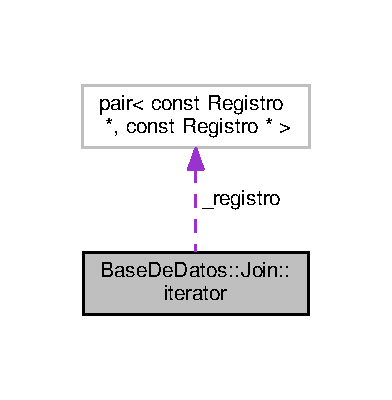
\includegraphics[width=188pt]{structBaseDeDatos_1_1Join_1_1iterator__coll__graph}
\end{center}
\end{figure}
\subsection*{Métodos públicos}
\begin{DoxyCompactItemize}
\item 
\hypertarget{structBaseDeDatos_1_1Join_1_1iterator_a3ffbdf64b1986e8f3bc745b754c7b538}{\hyperlink{structBaseDeDatos_1_1Join_1_1iterator}{iterator} \hyperlink{structBaseDeDatos_1_1Join_1_1iterator_a3ffbdf64b1986e8f3bc745b754c7b538}{operator++} ()}\label{structBaseDeDatos_1_1Join_1_1iterator_a3ffbdf64b1986e8f3bc745b754c7b538}

\begin{DoxyCompactList}\small\item\em Par de registros de las tabla 1 y 2, representando un registro del join entre ambas. \end{DoxyCompactList}\item 
\hypertarget{structBaseDeDatos_1_1Join_1_1iterator_a5b090095c29aad7e8b7c18d6d5e8b202}{\hyperlink{classRegistro}{Registro} \hyperlink{structBaseDeDatos_1_1Join_1_1iterator_a5b090095c29aad7e8b7c18d6d5e8b202}{operator$\ast$} ()}\label{structBaseDeDatos_1_1Join_1_1iterator_a5b090095c29aad7e8b7c18d6d5e8b202}

\begin{DoxyCompactList}\small\item\em Par de registros de las tabla 1 y 2, representando un registro del join entre ambas. \end{DoxyCompactList}\end{DoxyCompactItemize}
\subsection*{Atributos públicos}
\begin{DoxyCompactItemize}
\item 
\hypertarget{structBaseDeDatos_1_1Join_1_1iterator_ab4d4ccfde30f66e4f2063adecfce45b3}{pair$<$ const \hyperlink{classRegistro}{Registro} $\ast$, const \\*
\hyperlink{classRegistro}{Registro} $\ast$ $>$ $\ast$ \hyperlink{structBaseDeDatos_1_1Join_1_1iterator_ab4d4ccfde30f66e4f2063adecfce45b3}{\-\_\-registro}}\label{structBaseDeDatos_1_1Join_1_1iterator_ab4d4ccfde30f66e4f2063adecfce45b3}

\begin{DoxyCompactList}\small\item\em Par de registros de las tabla 1 y 2, representando un registro del join entre ambas. \end{DoxyCompactList}\end{DoxyCompactItemize}


La documentación para esta estructura fue generada a partir del siguiente fichero\-:\begin{DoxyCompactItemize}
\item 
src/Base\-De\-Datos.\-h\end{DoxyCompactItemize}

\hypertarget{classstring__map_1_1iterator}{\section{Referencia de la Clase string\-\_\-map$<$ T $>$\-:\-:iterator}
\label{classstring__map_1_1iterator}\index{string\-\_\-map$<$ T $>$\-::iterator@{string\-\_\-map$<$ T $>$\-::iterator}}
}


Diagrama de colaboración para string\-\_\-map$<$ T $>$\-:\-:iterator\-:
\nopagebreak
\begin{figure}[H]
\begin{center}
\leavevmode
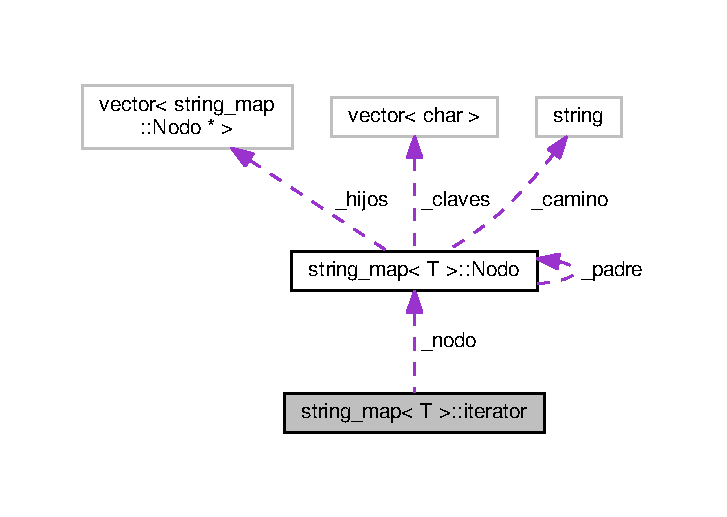
\includegraphics[width=349pt]{classstring__map_1_1iterator__coll__graph}
\end{center}
\end{figure}
\subsection*{Tipos públicos}
\begin{DoxyCompactItemize}
\item 
\hypertarget{classstring__map_1_1iterator_a82c72ceda356ce40c68ad689205fd225}{using {\bfseries value\-\_\-type} = \hyperlink{classstring__map}{string\-\_\-map}$<$ T $>$\-::value\-\_\-type}\label{classstring__map_1_1iterator_a82c72ceda356ce40c68ad689205fd225}

\item 
\hypertarget{classstring__map_1_1iterator_a2d813421047005b3fbf3e66b1e1f6535}{using {\bfseries reference} = value\-\_\-type \&}\label{classstring__map_1_1iterator_a2d813421047005b3fbf3e66b1e1f6535}

\item 
\hypertarget{classstring__map_1_1iterator_a3be8d54fc66efd989b16c38891c5d0fd}{using {\bfseries pointer} = value\-\_\-type $\ast$}\label{classstring__map_1_1iterator_a3be8d54fc66efd989b16c38891c5d0fd}

\end{DoxyCompactItemize}
\subsection*{Métodos públicos}
\begin{DoxyCompactItemize}
\item 
\hyperlink{classstring__map_1_1iterator_ab1891c4db11af26df474d6e512228da7}{iterator} (const typename \hyperlink{classstring__map}{string\-\_\-map}$<$ T $>$\-::\hyperlink{classstring__map_1_1iterator}{iterator} \&)
\begin{DoxyCompactList}\small\item\em Constructor por copia del iterador. \end{DoxyCompactList}\item 
\hyperlink{classstring__map_1_1iterator_a4102a117dc5f45345426017d1286f1ad}{iterator} (const typename \hyperlink{classstring__map}{string\-\_\-map}$<$ T $>$\-::\hyperlink{structstring__map_1_1Nodo}{Nodo} $\ast$)
\begin{DoxyCompactList}\small\item\em Constructor por refernecia a \hyperlink{structstring__map_1_1Nodo}{Nodo}. \end{DoxyCompactList}\item 
\hyperlink{classstring__map_1_1iterator}{iterator} \& \hyperlink{classstring__map_1_1iterator_ae0ccdb8ae9f8303956cb420c1d06a94d}{operator=} (const typename \hyperlink{classstring__map}{string\-\_\-map}$<$ T $>$\-::\hyperlink{classstring__map_1_1iterator}{iterator} \&)
\begin{DoxyCompactList}\small\item\em Constructor por copia del iterador. \end{DoxyCompactList}\item 
\hyperlink{classstring__map_1_1iterator}{iterator} \& \hyperlink{classstring__map_1_1iterator_a9532a114feb48b855c8d4baa86d6c99f}{operator++} ()
\begin{DoxyCompactList}\small\item\em Avanza el iterador una posición. \end{DoxyCompactList}\item 
value\-\_\-type \& \hyperlink{classstring__map_1_1iterator_a50e95502f262791747fee46b9d2784ec}{operator$\ast$} ()
\begin{DoxyCompactList}\small\item\em Desreferencia el puntero. \end{DoxyCompactList}\item 
\hypertarget{classstring__map_1_1iterator_ac24292b43be1abbb58c16e240a4b45e6}{bool {\bfseries definido} () const }\label{classstring__map_1_1iterator_ac24292b43be1abbb58c16e240a4b45e6}

\item 
value\-\_\-type $\ast$ \hyperlink{classstring__map_1_1iterator_a4fabcd1bf327adeff53dc52ccc0a8229}{operator-\/$>$} ()
\begin{DoxyCompactList}\small\item\em Operador flechita. \end{DoxyCompactList}\item 
bool \hyperlink{classstring__map_1_1iterator_ae925a84681f01ac54a40868a592486d1}{operator==} (const \hyperlink{classstring__map}{string\-\_\-map}$<$ T $>$\-::\hyperlink{classstring__map_1_1iterator}{iterator} \&other) const 
\begin{DoxyCompactList}\small\item\em Comparación entre iteradores. \end{DoxyCompactList}\item 
bool \hyperlink{classstring__map_1_1iterator_a6b5de52586495286a8c211759667387c}{operator!=} (const \hyperlink{classstring__map}{string\-\_\-map}$<$ T $>$\-::\hyperlink{classstring__map_1_1iterator}{iterator} \&other) const 
\begin{DoxyCompactList}\small\item\em Comparación entre iteradores. \end{DoxyCompactList}\end{DoxyCompactItemize}
\subsection*{Métodos privados}
\begin{DoxyCompactItemize}
\item 
\hypertarget{classstring__map_1_1iterator_a9adc687055baa860aaddb8f2f955ae1a}{\hyperlink{classstring__map_1_1iterator_a9adc687055baa860aaddb8f2f955ae1a}{iterator} (\hyperlink{structstring__map_1_1Nodo}{Nodo} $\ast$n)}\label{classstring__map_1_1iterator_a9adc687055baa860aaddb8f2f955ae1a}

\begin{DoxyCompactList}\small\item\em El iterador es puntero a \hyperlink{structstring__map_1_1Nodo}{Nodo}. \end{DoxyCompactList}\end{DoxyCompactItemize}
\subsection*{Atributos privados}
\begin{DoxyCompactItemize}
\item 
\hypertarget{classstring__map_1_1iterator_aa1f7fdb1686ce1b763c002490fc83c51}{\hyperlink{structstring__map_1_1Nodo}{Nodo} $\ast$ {\bfseries \-\_\-nodo}}\label{classstring__map_1_1iterator_aa1f7fdb1686ce1b763c002490fc83c51}

\end{DoxyCompactItemize}
\subsection*{Amigas}
\begin{DoxyCompactItemize}
\item 
\hypertarget{classstring__map_1_1iterator_ad0a70c0d4333f3435a234a4682421708}{class {\bfseries string\-\_\-map$<$ T $>$}}\label{classstring__map_1_1iterator_ad0a70c0d4333f3435a234a4682421708}

\end{DoxyCompactItemize}


\subsection{Documentación del constructor y destructor}
\hypertarget{classstring__map_1_1iterator_ab1891c4db11af26df474d6e512228da7}{\index{string\-\_\-map\-::iterator@{string\-\_\-map\-::iterator}!iterator@{iterator}}
\index{iterator@{iterator}!string_map::iterator@{string\-\_\-map\-::iterator}}
\subsubsection[{iterator}]{\setlength{\rightskip}{0pt plus 5cm}template$<$typename T$>$ {\bf string\-\_\-map}$<$ T $>$\-::iterator\-::iterator (
\begin{DoxyParamCaption}
\item[{const typename {\bf string\-\_\-map}$<$ T $>$\-::{\bf iterator} \&}]{}
\end{DoxyParamCaption}
)}}\label{classstring__map_1_1iterator_ab1891c4db11af26df474d6e512228da7}


Constructor por copia del iterador. 


\begin{DoxyDescription}
\item[Complejidad Temporal]$O$(1)
\end{DoxyDescription}\hypertarget{classstring__map_1_1iterator_a4102a117dc5f45345426017d1286f1ad}{\index{string\-\_\-map\-::iterator@{string\-\_\-map\-::iterator}!iterator@{iterator}}
\index{iterator@{iterator}!string_map::iterator@{string\-\_\-map\-::iterator}}
\subsubsection[{iterator}]{\setlength{\rightskip}{0pt plus 5cm}template$<$typename T$>$ {\bf string\-\_\-map}$<$ T $>$\-::iterator\-::iterator (
\begin{DoxyParamCaption}
\item[{const typename {\bf string\-\_\-map}$<$ T $>$\-::{\bf Nodo} $\ast$}]{}
\end{DoxyParamCaption}
)}}\label{classstring__map_1_1iterator_a4102a117dc5f45345426017d1286f1ad}


Constructor por refernecia a \hyperlink{structstring__map_1_1Nodo}{Nodo}. 


\begin{DoxyDescription}
\item[Complejidad Temporal]$O$(1)
\end{DoxyDescription}

\subsection{Documentación de las funciones miembro}
\hypertarget{classstring__map_1_1iterator_a6b5de52586495286a8c211759667387c}{\index{string\-\_\-map\-::iterator@{string\-\_\-map\-::iterator}!operator!=@{operator!=}}
\index{operator!=@{operator!=}!string_map::iterator@{string\-\_\-map\-::iterator}}
\subsubsection[{operator!=}]{\setlength{\rightskip}{0pt plus 5cm}template$<$typename T$>$ bool {\bf string\-\_\-map}$<$ T $>$\-::iterator\-::operator!= (
\begin{DoxyParamCaption}
\item[{const {\bf string\-\_\-map}$<$ T $>$\-::{\bf iterator} \&}]{other}
\end{DoxyParamCaption}
) const}}\label{classstring__map_1_1iterator_a6b5de52586495286a8c211759667387c}


Comparación entre iteradores. 

\begin{DoxyPrecond}{Precondición}
ambos iteradores refieren a la misma colección 
\end{DoxyPrecond}
\begin{DoxyPostcond}{Postcondición}
true sii los iteradores no apuntan al mismo elemento
\end{DoxyPostcond}

\begin{DoxyDescription}
\item[Complejidad Temporal]$O$(1)
\end{DoxyDescription}\hypertarget{classstring__map_1_1iterator_a50e95502f262791747fee46b9d2784ec}{\index{string\-\_\-map\-::iterator@{string\-\_\-map\-::iterator}!operator$\ast$@{operator$\ast$}}
\index{operator$\ast$@{operator$\ast$}!string_map::iterator@{string\-\_\-map\-::iterator}}
\subsubsection[{operator$\ast$}]{\setlength{\rightskip}{0pt plus 5cm}template$<$typename T$>$ {\bf string\-\_\-map}$<$ T $>$\-::iterator\-::value\-\_\-type \& {\bf string\-\_\-map}$<$ T $>$\-::iterator\-::operator$\ast$ (
\begin{DoxyParamCaption}
{}
\end{DoxyParamCaption}
)}}\label{classstring__map_1_1iterator_a50e95502f262791747fee46b9d2784ec}


Desreferencia el puntero. 

El valor devuelto tiene aliasing dentro de la colección.

\begin{DoxyPrecond}{Precondición}
El iterador no debe estar en la posición pasando-\/el-\/último. 
\end{DoxyPrecond}
\begin{DoxyPostcond}{Postcondición}
El valor resultado es una referencia al valor apuntado.
\end{DoxyPostcond}

\begin{DoxyDescription}
\item[Complejidad Temporal]$O$(1)
\end{DoxyDescription}\hypertarget{classstring__map_1_1iterator_a9532a114feb48b855c8d4baa86d6c99f}{\index{string\-\_\-map\-::iterator@{string\-\_\-map\-::iterator}!operator++@{operator++}}
\index{operator++@{operator++}!string_map::iterator@{string\-\_\-map\-::iterator}}
\subsubsection[{operator++}]{\setlength{\rightskip}{0pt plus 5cm}template$<$typename T$>$ {\bf string\-\_\-map}$<$ T $>$\-::{\bf iterator} \& {\bf string\-\_\-map}$<$ T $>$\-::iterator\-::operator++ (
\begin{DoxyParamCaption}
{}
\end{DoxyParamCaption}
)}}\label{classstring__map_1_1iterator_a9532a114feb48b855c8d4baa86d6c99f}


Avanza el iterador una posición. 

\begin{DoxyPrecond}{Precondición}
El iterador no debe estar en la posición pasando-\/el-\/último. 
\end{DoxyPrecond}
\begin{DoxyPostcond}{Postcondición}
{\bfseries res} es una referencia a {\bfseries this}. {\bfseries this} apunta a la posición siguiente.
\end{DoxyPostcond}

\begin{DoxyDescription}
\item[Complejidad Temporal]$O$(1)
\end{DoxyDescription}\hypertarget{classstring__map_1_1iterator_a4fabcd1bf327adeff53dc52ccc0a8229}{\index{string\-\_\-map\-::iterator@{string\-\_\-map\-::iterator}!operator-\/$>$@{operator-\/$>$}}
\index{operator-\/$>$@{operator-\/$>$}!string_map::iterator@{string\-\_\-map\-::iterator}}
\subsubsection[{operator-\/$>$}]{\setlength{\rightskip}{0pt plus 5cm}template$<$typename T$>$ {\bf string\-\_\-map}$<$ T $>$\-::iterator\-::value\-\_\-type $\ast$ {\bf string\-\_\-map}$<$ T $>$\-::iterator\-::operator-\/$>$ (
\begin{DoxyParamCaption}
{}
\end{DoxyParamCaption}
)}}\label{classstring__map_1_1iterator_a4fabcd1bf327adeff53dc52ccc0a8229}


Operador flechita. 

El valor devuelvo tiene aliasing dentro de la colección.

\begin{DoxyPrecond}{Precondición}
El iterador no debe estar en la posición pasando-\/el-\/último. 
\end{DoxyPrecond}
\begin{DoxyPostcond}{Postcondición}
El valor resultado es un puntero al valor apuntado.
\end{DoxyPostcond}

\begin{DoxyDescription}
\item[Complejidad Temporal]$O$(1)
\end{DoxyDescription}\hypertarget{classstring__map_1_1iterator_ae0ccdb8ae9f8303956cb420c1d06a94d}{\index{string\-\_\-map\-::iterator@{string\-\_\-map\-::iterator}!operator=@{operator=}}
\index{operator=@{operator=}!string_map::iterator@{string\-\_\-map\-::iterator}}
\subsubsection[{operator=}]{\setlength{\rightskip}{0pt plus 5cm}template$<$typename T$>$ {\bf string\-\_\-map}$<$ T $>$\-::{\bf iterator} \& {\bf string\-\_\-map}$<$ T $>$\-::iterator\-::operator= (
\begin{DoxyParamCaption}
\item[{const typename {\bf string\-\_\-map}$<$ T $>$\-::{\bf iterator} \&}]{}
\end{DoxyParamCaption}
)}}\label{classstring__map_1_1iterator_ae0ccdb8ae9f8303956cb420c1d06a94d}


Constructor por copia del iterador. 


\begin{DoxyDescription}
\item[Complejidad Temporal]$O$(1)
\end{DoxyDescription}\hypertarget{classstring__map_1_1iterator_ae925a84681f01ac54a40868a592486d1}{\index{string\-\_\-map\-::iterator@{string\-\_\-map\-::iterator}!operator==@{operator==}}
\index{operator==@{operator==}!string_map::iterator@{string\-\_\-map\-::iterator}}
\subsubsection[{operator==}]{\setlength{\rightskip}{0pt plus 5cm}template$<$typename T$>$ bool {\bf string\-\_\-map}$<$ T $>$\-::iterator\-::operator== (
\begin{DoxyParamCaption}
\item[{const {\bf string\-\_\-map}$<$ T $>$\-::{\bf iterator} \&}]{other}
\end{DoxyParamCaption}
) const}}\label{classstring__map_1_1iterator_ae925a84681f01ac54a40868a592486d1}


Comparación entre iteradores. 

\begin{DoxyPrecond}{Precondición}
ambos iteradores refieren a la misma colección 
\end{DoxyPrecond}
\begin{DoxyPostcond}{Postcondición}
true sii los iteradores apuntan al mismo elemento
\end{DoxyPostcond}

\begin{DoxyDescription}
\item[Complejidad Temporal]$O$(1)
\end{DoxyDescription}

La documentación para esta clase fue generada a partir del siguiente fichero\-:\begin{DoxyCompactItemize}
\item 
src/string\-\_\-map\-\_\-iterators.\-h\end{DoxyCompactItemize}

\hypertarget{structBaseDeDatos_1_1Join}{\section{Referencia de la Estructura Base\-De\-Datos\-:\-:Join}
\label{structBaseDeDatos_1_1Join}\index{Base\-De\-Datos\-::\-Join@{Base\-De\-Datos\-::\-Join}}
}


\hyperlink{structBaseDeDatos_1_1Join}{Join} entre dos tablas Para cada clave del diccionario (registros de tabla1) tengo los registros de tabla2 que coinciden en el campo dado.  




Diagrama de colaboración para Base\-De\-Datos\-:\-:Join\-:
\nopagebreak
\begin{figure}[H]
\begin{center}
\leavevmode
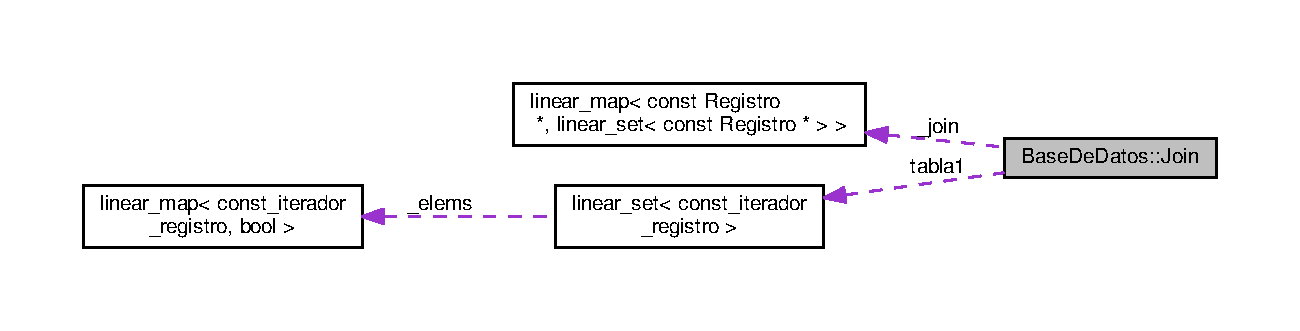
\includegraphics[width=350pt]{structBaseDeDatos_1_1Join__coll__graph}
\end{center}
\end{figure}
\subsection*{Clases}
\begin{DoxyCompactItemize}
\item 
struct \hyperlink{structBaseDeDatos_1_1Join_1_1iterator}{iterator}
\end{DoxyCompactItemize}
\subsection*{Métodos públicos}
\begin{DoxyCompactItemize}
\item 
\hypertarget{structBaseDeDatos_1_1Join_a21a90ab59b29952f615a3d793c103a73}{\hyperlink{structBaseDeDatos_1_1Join_1_1iterator}{iterator} \hyperlink{structBaseDeDatos_1_1Join_a21a90ab59b29952f615a3d793c103a73}{begin} ()}\label{structBaseDeDatos_1_1Join_a21a90ab59b29952f615a3d793c103a73}

\begin{DoxyCompactList}\small\item\em Devuelve un iterador al primer elemento. \end{DoxyCompactList}\item 
\hypertarget{structBaseDeDatos_1_1Join_adc880cc8af0728b926d2f1ff7db8443c}{\hyperlink{structBaseDeDatos_1_1Join_1_1iterator}{iterator} \hyperlink{structBaseDeDatos_1_1Join_adc880cc8af0728b926d2f1ff7db8443c}{end} ()}\label{structBaseDeDatos_1_1Join_adc880cc8af0728b926d2f1ff7db8443c}

\begin{DoxyCompactList}\small\item\em Devuelve un iterador al ultimo elemento. \end{DoxyCompactList}\end{DoxyCompactItemize}
\subsection*{Atributos públicos}
\begin{DoxyCompactItemize}
\item 
\hypertarget{structBaseDeDatos_1_1Join_aa40d69dd6bfd4281b0aeb3f192730825}{\hyperlink{classlinear__map}{linear\-\_\-map}$<$ const \hyperlink{classRegistro}{Registro} \\*
$\ast$, \hyperlink{classlinear__set}{linear\-\_\-set}$<$ const \hyperlink{classRegistro}{Registro} $\ast$ $>$ $>$ \hyperlink{structBaseDeDatos_1_1Join_aa40d69dd6bfd4281b0aeb3f192730825}{\-\_\-join}}\label{structBaseDeDatos_1_1Join_aa40d69dd6bfd4281b0aeb3f192730825}

\begin{DoxyCompactList}\small\item\em Diccionario que define las relaciones entre los registros de dos tablas a unir. \end{DoxyCompactList}\item 
\hypertarget{structBaseDeDatos_1_1Join_a20248fc0e89786c08c27e22ee4053ffb}{\hyperlink{classlinear__set}{linear\-\_\-set}\\*
$<$ const\-\_\-iterador\-\_\-registro $>$ {\bfseries tabla1}}\label{structBaseDeDatos_1_1Join_a20248fc0e89786c08c27e22ee4053ffb}

\end{DoxyCompactItemize}


\subsection{Descripción detallada}
\hyperlink{structBaseDeDatos_1_1Join}{Join} entre dos tablas Para cada clave del diccionario (registros de tabla1) tengo los registros de tabla2 que coinciden en el campo dado. 

La documentación para esta estructura fue generada a partir de los siguientes ficheros\-:\begin{DoxyCompactItemize}
\item 
src/Base\-De\-Datos.\-h\item 
src/Base\-De\-Datos.\-cpp\end{DoxyCompactItemize}

\hypertarget{classlinear__map}{\section{Referencia de la plantilla de la Clase linear\-\_\-map$<$ K, S $>$}
\label{classlinear__map}\index{linear\-\_\-map$<$ K, S $>$@{linear\-\_\-map$<$ K, S $>$}}
}


Módulo diccionario con inserción en O(1)  




{\ttfamily \#include $<$linear\-\_\-map.\-h$>$}

\subsection*{Tipos públicos}
\begin{DoxyCompactItemize}
\item 
\hypertarget{classlinear__map_a85577f6aa54870bf9b5d2f85f0749078}{using {\bfseries key\-\_\-type} = K}\label{classlinear__map_a85577f6aa54870bf9b5d2f85f0749078}

\item 
\hypertarget{classlinear__map_aaed4a6810a4a46c0cede18821069cc65}{using {\bfseries mapped\-\_\-type} = S}\label{classlinear__map_aaed4a6810a4a46c0cede18821069cc65}

\item 
\hypertarget{classlinear__map_a8bf7640c132d7e6fa5c4e68e1623d27d}{using {\bfseries value\-\_\-type} = pair$<$ const K, S $>$}\label{classlinear__map_a8bf7640c132d7e6fa5c4e68e1623d27d}

\item 
\hypertarget{classlinear__map_a08095dfd88596e72f10d59a212b622f8}{using {\bfseries size\-\_\-type} = size\-\_\-t}\label{classlinear__map_a08095dfd88596e72f10d59a212b622f8}

\item 
\hypertarget{classlinear__map_a26639947def2ce8549cde3fdd31bd42e}{using {\bfseries iterator} = typename list$<$ pair$<$ const K, S $>$$>$\-::iterator}\label{classlinear__map_a26639947def2ce8549cde3fdd31bd42e}

\item 
\hypertarget{classlinear__map_ae4a408774a63cf33acbb0397b64972e5}{using {\bfseries const\-\_\-iterator} = typename list$<$ pair$<$ const K, S $>$$>$\-::const\-\_\-iterator}\label{classlinear__map_ae4a408774a63cf33acbb0397b64972e5}

\end{DoxyCompactItemize}
\subsection*{Métodos públicos}
\begin{DoxyCompactItemize}
\item 
\hyperlink{classlinear__map_a2343174c5c974fefcec889b0954debcf}{linear\-\_\-map} ()
\begin{DoxyCompactList}\small\item\em Crea un diccionario vacio. \end{DoxyCompactList}\item 
\hyperlink{classlinear__map_a29a92ea4bf65d4f5936b061ebb8309fa}{linear\-\_\-map} (const \hyperlink{classlinear__map}{linear\-\_\-map}$<$ K, S $>$ \&other)
\begin{DoxyCompactList}\small\item\em Constructor por copia. \end{DoxyCompactList}\item 
pair$<$ iterator, bool $>$ \hyperlink{classlinear__map_a3631b2f824bbf4489943f0816464068e}{insert} (const value\-\_\-type \&v)
\begin{DoxyCompactList}\small\item\em Define o redefine una relación en el diccionario. \end{DoxyCompactList}\item 
iterator \hyperlink{classlinear__map_a6f04a74f63434402f7198aaac798d9da}{fast\-\_\-insert} (const value\-\_\-type \&v)
\begin{DoxyCompactList}\small\item\em Define una nueva relación en el diccionario. \end{DoxyCompactList}\item 
size\-\_\-type \hyperlink{classlinear__map_a16f411ae0221b803418d63862b6f3223}{size} () const 
\begin{DoxyCompactList}\small\item\em Tamaño del diccionario. \end{DoxyCompactList}\item 
S \& \hyperlink{classlinear__map_ad528c5b74bb14cfe7170bffffce2e979}{at} (const K \&key)
\begin{DoxyCompactList}\small\item\em Devuelve el significado relacionado con la clave. \end{DoxyCompactList}\item 
bool \hyperlink{classlinear__map_a8246ed178b7e0747d973c5bf6a0e690f}{empty} () const 
\begin{DoxyCompactList}\small\item\em True si el diccionario está vacío. \end{DoxyCompactList}\item 
iterator \hyperlink{classlinear__map_a227924393723570ac58f79fd194aac61}{find} (const K \&k)
\begin{DoxyCompactList}\small\item\em Devuelve un iterador relacionado a la clave buscada. End si no está definida. \end{DoxyCompactList}\item 
const\-\_\-iterator \hyperlink{classlinear__map_a30492a8c9ad1cef02185a9a6ce439114}{find} (const K \&k) const 
\begin{DoxyCompactList}\small\item\em Devuelve un iterador const relacionado a la clave buscada. End si no está definida. \end{DoxyCompactList}\item 
iterator \hyperlink{classlinear__map_a88a219ae647727d1b7e67c2dbe36d972}{begin} ()
\begin{DoxyCompactList}\small\item\em Devuelve un iterador al inicio del diccionario. \end{DoxyCompactList}\item 
iterator \hyperlink{classlinear__map_a29f90bee46581029b6ce496d4ea46683}{end} ()
\begin{DoxyCompactList}\small\item\em Devuelve un iterador a la posición pasando-\/el-\/último. \end{DoxyCompactList}\item 
const\-\_\-iterator \hyperlink{classlinear__map_a583872ffc15171c0d7c3caf307d2d9fe}{begin} () const 
\begin{DoxyCompactList}\small\item\em Devuelve un iterador const al inicio del diccionario. \end{DoxyCompactList}\item 
const\-\_\-iterator \hyperlink{classlinear__map_a0839117b87a8ad0a340df43c942779ad}{end} () const 
\begin{DoxyCompactList}\small\item\em Devuelve un iterador const a la posición pasando-\/el-\/último. \end{DoxyCompactList}\item 
size\-\_\-t \hyperlink{classlinear__map_a99fb7cbd872a6536bcdf00a16255533a}{count} (const K \&k) const 
\begin{DoxyCompactList}\small\item\em Cantidad de apariciones de la clave. \end{DoxyCompactList}\item 
const S \& \hyperlink{classlinear__map_a7bbfefc3467a2f178c069b3958e81c8a}{at} (const K \&key) const 
\begin{DoxyCompactList}\small\item\em Devuelve el significado relacionado con la clave. \end{DoxyCompactList}\item 
size\-\_\-type \hyperlink{classlinear__map_a932198aa420701fb84af74434764be9d}{erase} (const K \&key)
\begin{DoxyCompactList}\small\item\em Elimina el significado del diccionario. Devuelve la cantidad de elementos elminados. \end{DoxyCompactList}\item 
\hyperlink{classlinear__map}{linear\-\_\-map} \& \hyperlink{classlinear__map_a9868e2ada8b775c57521506fe7dd24a7}{operator=} (const \hyperlink{classlinear__map}{linear\-\_\-map} \&other)
\begin{DoxyCompactList}\small\item\em Operador asignación del diccionario. \end{DoxyCompactList}\item 
bool \hyperlink{classlinear__map_aba00da27993faf7b3bf2b2e42203afbf}{operator==} (const \hyperlink{classlinear__map}{linear\-\_\-map} \&other) const 
\begin{DoxyCompactList}\small\item\em True si los diccionarios son iguales. \end{DoxyCompactList}\end{DoxyCompactItemize}
\subsection*{Atributos privados}
\begin{Indent}{\bf Representación\-:}\par
{\em rep\-: \hyperlink{classlinear__map}{linear\-\_\-map(\-Clave, Significado)} $\to$ bool\par
rep(d) $\equiv$
\begin{DoxyItemize}
\item $\forall$ (i, j \-: Nat) (0 $\leq$ i, j $<$ long(\-\_\-elems) $\land$ $\pi_1$(\-\_\-elems\mbox{[}i\mbox{]}) == $\pi_1$(\-\_\-elems\mbox{[}j\mbox{]})) $\Rightarrow$ i = j
\end{DoxyItemize}

$\bullet$ \mbox{[} $\bullet$\mbox{]} \-: Secu( $\alpha$) s $\times$ Nat i $\rightarrow$ $\alpha$ \{0 $\leq$ i $<$ long(s)\} \par
s\mbox{[}i\mbox{]} $\equiv$ {\bfseries if} i = 0 {\bfseries then} prim(s) {\bfseries else} fin(s)\mbox{[}i -\/ 1\mbox{]} {\bfseries fi} 

abs\-: \hyperlink{classlinear__map}{linear\-\_\-map(\-Clave, Significado)} $\to$ Dicc(\-Clave, Significado)\par
abs(d) $\equiv$ d' $|$
\begin{DoxyItemize}
\item $\forall$ (c \-: Clave) def?(c, d') $\Leftrightarrow$ $\exists$ (t \-: tupla(\-Clave, Significado)) está?(t, \-\_\-elems) $\land$ P1(t) == c
\item $\forall$ (t \-: tupla(\-Clave, Significado)) está?(t, \-\_\-elems) $\Rightarrow$ P2(t) == obtener(P1(t), d') 
\end{DoxyItemize}}\begin{DoxyCompactItemize}
\item 
\hypertarget{classlinear__map_aeb6846d41a9b28c5511b1ece965efe61}{list$<$ pair$<$ const K, S $>$ $>$ {\bfseries \-\_\-elems}}\label{classlinear__map_aeb6846d41a9b28c5511b1ece965efe61}

\end{DoxyCompactItemize}
\end{Indent}


\subsection{Descripción detallada}
\subsubsection*{template$<$class K, class S$>$class linear\-\_\-map$<$ K, S $>$}

Módulo diccionario con inserción en O(1) 


\begin{DoxyTemplParams}{Template Parameters}
{\em K} & tipo paramétrico para la clave \\
\hline
{\em S} & tipo paramétrico para el significado\\
\hline
\end{DoxyTemplParams}
Se espera que K tenga\-:
\begin{DoxyItemize}
\item operator==
\item Constructor por copia
\end{DoxyItemize}

Se espera que S tenga\-:
\begin{DoxyItemize}
\item Constructor por copoa
\end{DoxyItemize}

{\bfseries se explica con} T\-A\-D Diccionario(\-K, S) 

\subsection{Documentación del constructor y destructor}
\hypertarget{classlinear__map_a2343174c5c974fefcec889b0954debcf}{\index{linear\-\_\-map@{linear\-\_\-map}!linear\-\_\-map@{linear\-\_\-map}}
\index{linear\-\_\-map@{linear\-\_\-map}!linear_map@{linear\-\_\-map}}
\subsubsection[{linear\-\_\-map}]{\setlength{\rightskip}{0pt plus 5cm}template$<$class K , class S $>$ {\bf linear\-\_\-map}$<$ K, S $>$\-::{\bf linear\-\_\-map} (
\begin{DoxyParamCaption}
{}
\end{DoxyParamCaption}
)}}\label{classlinear__map_a2343174c5c974fefcec889b0954debcf}


Crea un diccionario vacio. 

\begin{DoxyPrecond}{Precondición}
true 
\end{DoxyPrecond}
\begin{DoxyPostcond}{Postcondición}
{\bfseries this} = vacio
\end{DoxyPostcond}

\begin{DoxyDescription}
\item[Complejidad Temporal]$O$(1)
\end{DoxyDescription}\hypertarget{classlinear__map_a29a92ea4bf65d4f5936b061ebb8309fa}{\index{linear\-\_\-map@{linear\-\_\-map}!linear\-\_\-map@{linear\-\_\-map}}
\index{linear\-\_\-map@{linear\-\_\-map}!linear_map@{linear\-\_\-map}}
\subsubsection[{linear\-\_\-map}]{\setlength{\rightskip}{0pt plus 5cm}template$<$class K, class S$>$ {\bf linear\-\_\-map}$<$ K, S $>$\-::{\bf linear\-\_\-map} (
\begin{DoxyParamCaption}
\item[{const {\bf linear\-\_\-map}$<$ K, S $>$ \&}]{other}
\end{DoxyParamCaption}
)}}\label{classlinear__map_a29a92ea4bf65d4f5936b061ebb8309fa}


Constructor por copia. 

\begin{DoxyPrecond}{Precondición}
true 
\end{DoxyPrecond}
\begin{DoxyPostcond}{Postcondición}
{\bfseries this} es una copia de other. No hay aliasing.
\end{DoxyPostcond}

\begin{DoxyDescription}
\item[Complejidad Temporal]$O$(\#claves(ohter) $\ast$ (copy(\-Clave) + copy(\-Significado)))
\end{DoxyDescription}

\subsection{Documentación de las funciones miembro}
\hypertarget{classlinear__map_ad528c5b74bb14cfe7170bffffce2e979}{\index{linear\-\_\-map@{linear\-\_\-map}!at@{at}}
\index{at@{at}!linear_map@{linear\-\_\-map}}
\subsubsection[{at}]{\setlength{\rightskip}{0pt plus 5cm}template$<$class K, class S $>$ S \& {\bf linear\-\_\-map}$<$ K, S $>$\-::at (
\begin{DoxyParamCaption}
\item[{const K \&}]{key}
\end{DoxyParamCaption}
)}}\label{classlinear__map_ad528c5b74bb14cfe7170bffffce2e979}


Devuelve el significado relacionado con la clave. 

El significado se devuelve por referencia modificable.

\begin{DoxyPrecond}{Precondición}
def?(key, {\bfseries this}) 
\end{DoxyPrecond}
\begin{DoxyPostcond}{Postcondición}
{\bfseries res} = obtener({\bfseries this}, k)
\end{DoxyPostcond}

\begin{DoxyDescription}
\item[Complejidad Temporal]$O$(\#claves({\bfseries this}))
\end{DoxyDescription}\hypertarget{classlinear__map_a7bbfefc3467a2f178c069b3958e81c8a}{\index{linear\-\_\-map@{linear\-\_\-map}!at@{at}}
\index{at@{at}!linear_map@{linear\-\_\-map}}
\subsubsection[{at}]{\setlength{\rightskip}{0pt plus 5cm}template$<$class K, class S $>$ const S \& {\bf linear\-\_\-map}$<$ K, S $>$\-::at (
\begin{DoxyParamCaption}
\item[{const K \&}]{key}
\end{DoxyParamCaption}
) const}}\label{classlinear__map_a7bbfefc3467a2f178c069b3958e81c8a}


Devuelve el significado relacionado con la clave. 

El significado se devuelve por referencia no-\/modificable.

\begin{DoxyPrecond}{Precondición}
def?(key, {\bfseries this}) 
\end{DoxyPrecond}
\begin{DoxyPostcond}{Postcondición}
{\bfseries res} = obtener({\bfseries this}, k)
\end{DoxyPostcond}

\begin{DoxyDescription}
\item[Complejidad Temporal]$O$(\#claves({\bfseries this}))
\end{DoxyDescription}\hypertarget{classlinear__map_a88a219ae647727d1b7e67c2dbe36d972}{\index{linear\-\_\-map@{linear\-\_\-map}!begin@{begin}}
\index{begin@{begin}!linear_map@{linear\-\_\-map}}
\subsubsection[{begin}]{\setlength{\rightskip}{0pt plus 5cm}template$<$class K , class S $>$ {\bf linear\-\_\-map}$<$ K, S $>$\-::iterator {\bf linear\-\_\-map}$<$ K, S $>$\-::begin (
\begin{DoxyParamCaption}
{}
\end{DoxyParamCaption}
)}}\label{classlinear__map_a88a219ae647727d1b7e67c2dbe36d972}


Devuelve un iterador al inicio del diccionario. 

\begin{DoxyPrecond}{Precondición}
true 
\end{DoxyPrecond}
\begin{DoxyPostcond}{Postcondición}
{\bfseries res} apunta al inicio del diccionario
\end{DoxyPostcond}

\begin{DoxyDescription}
\item[Complejidad Temporal]$O$(1)
\end{DoxyDescription}\hypertarget{classlinear__map_a583872ffc15171c0d7c3caf307d2d9fe}{\index{linear\-\_\-map@{linear\-\_\-map}!begin@{begin}}
\index{begin@{begin}!linear_map@{linear\-\_\-map}}
\subsubsection[{begin}]{\setlength{\rightskip}{0pt plus 5cm}template$<$class K , class S $>$ {\bf linear\-\_\-map}$<$ K, S $>$\-::const\-\_\-iterator {\bf linear\-\_\-map}$<$ K, S $>$\-::begin (
\begin{DoxyParamCaption}
{}
\end{DoxyParamCaption}
) const}}\label{classlinear__map_a583872ffc15171c0d7c3caf307d2d9fe}


Devuelve un iterador const al inicio del diccionario. 

\begin{DoxyPrecond}{Precondición}
true 
\end{DoxyPrecond}
\begin{DoxyPostcond}{Postcondición}
{\bfseries res} apunta al inicio del diccionario
\end{DoxyPostcond}

\begin{DoxyDescription}
\item[Complejidad Temporal]$O$(1)
\end{DoxyDescription}\hypertarget{classlinear__map_a99fb7cbd872a6536bcdf00a16255533a}{\index{linear\-\_\-map@{linear\-\_\-map}!count@{count}}
\index{count@{count}!linear_map@{linear\-\_\-map}}
\subsubsection[{count}]{\setlength{\rightskip}{0pt plus 5cm}template$<$class K, class S $>$ size\-\_\-t {\bf linear\-\_\-map}$<$ K, S $>$\-::count (
\begin{DoxyParamCaption}
\item[{const K \&}]{k}
\end{DoxyParamCaption}
) const}}\label{classlinear__map_a99fb7cbd872a6536bcdf00a16255533a}


Cantidad de apariciones de la clave. 

\begin{DoxyPrecond}{Precondición}
true 
\end{DoxyPrecond}
\begin{DoxyPostcond}{Postcondición}
{\bfseries if} def?({\bfseries this}, k) {\bfseries then} {\bfseries res} = 1 {\bfseries else} {\bfseries res} = 0 {\bfseries fi} 
\end{DoxyPostcond}

\begin{DoxyDescription}
\item[Complejidad Temporal]$O$(\#claves({\bfseries this}) $\ast$ cmp(\-Clave)
\end{DoxyDescription}\hypertarget{classlinear__map_a8246ed178b7e0747d973c5bf6a0e690f}{\index{linear\-\_\-map@{linear\-\_\-map}!empty@{empty}}
\index{empty@{empty}!linear_map@{linear\-\_\-map}}
\subsubsection[{empty}]{\setlength{\rightskip}{0pt plus 5cm}template$<$class K, class S$>$ bool {\bf linear\-\_\-map}$<$ K, S $>$\-::empty (
\begin{DoxyParamCaption}
{}
\end{DoxyParamCaption}
) const\hspace{0.3cm}{\ttfamily [inline]}}}\label{classlinear__map_a8246ed178b7e0747d973c5bf6a0e690f}


True si el diccionario está vacío. 

\begin{DoxyPrecond}{Precondición}
true 
\end{DoxyPrecond}
\begin{DoxyPostcond}{Postcondición}
{\bfseries res} = $\emptyset$?(claves({\bfseries this}))
\end{DoxyPostcond}

\begin{DoxyDescription}
\item[Complejidad Temporal]$O$(1)
\end{DoxyDescription}\hypertarget{classlinear__map_a29f90bee46581029b6ce496d4ea46683}{\index{linear\-\_\-map@{linear\-\_\-map}!end@{end}}
\index{end@{end}!linear_map@{linear\-\_\-map}}
\subsubsection[{end}]{\setlength{\rightskip}{0pt plus 5cm}template$<$class K , class S $>$ {\bf linear\-\_\-map}$<$ K, S $>$\-::iterator {\bf linear\-\_\-map}$<$ K, S $>$\-::end (
\begin{DoxyParamCaption}
{}
\end{DoxyParamCaption}
)}}\label{classlinear__map_a29f90bee46581029b6ce496d4ea46683}


Devuelve un iterador a la posición pasando-\/el-\/último. 

\begin{DoxyPrecond}{Precondición}
true 
\end{DoxyPrecond}
\begin{DoxyPostcond}{Postcondición}
{\bfseries res} apunta a la posición pasando-\/el-\/último
\end{DoxyPostcond}

\begin{DoxyDescription}
\item[Complejidad Temporal]$O$(1)
\end{DoxyDescription}\hypertarget{classlinear__map_a0839117b87a8ad0a340df43c942779ad}{\index{linear\-\_\-map@{linear\-\_\-map}!end@{end}}
\index{end@{end}!linear_map@{linear\-\_\-map}}
\subsubsection[{end}]{\setlength{\rightskip}{0pt plus 5cm}template$<$class K , class S $>$ {\bf linear\-\_\-map}$<$ K, S $>$\-::const\-\_\-iterator {\bf linear\-\_\-map}$<$ K, S $>$\-::end (
\begin{DoxyParamCaption}
{}
\end{DoxyParamCaption}
) const}}\label{classlinear__map_a0839117b87a8ad0a340df43c942779ad}


Devuelve un iterador const a la posición pasando-\/el-\/último. 

\begin{DoxyPrecond}{Precondición}
true 
\end{DoxyPrecond}
\begin{DoxyPostcond}{Postcondición}
{\bfseries res} apunta a la posición pasando-\/el-\/último
\end{DoxyPostcond}

\begin{DoxyDescription}
\item[Complejidad Temporal]$O$(1)
\end{DoxyDescription}\hypertarget{classlinear__map_a932198aa420701fb84af74434764be9d}{\index{linear\-\_\-map@{linear\-\_\-map}!erase@{erase}}
\index{erase@{erase}!linear_map@{linear\-\_\-map}}
\subsubsection[{erase}]{\setlength{\rightskip}{0pt plus 5cm}template$<$class K, class S $>$ {\bf linear\-\_\-map}$<$ K, S $>$\-::size\-\_\-type {\bf linear\-\_\-map}$<$ K, S $>$\-::erase (
\begin{DoxyParamCaption}
\item[{const K \&}]{key}
\end{DoxyParamCaption}
)}}\label{classlinear__map_a932198aa420701fb84af74434764be9d}


Elimina el significado del diccionario. Devuelve la cantidad de elementos elminados. 

\begin{DoxyPrecond}{Precondición}
d == {\bfseries this} $\land$ def?(key, {\bfseries this}) 
\end{DoxyPrecond}
\begin{DoxyPostcond}{Postcondición}
{\bfseries this} == borrar(key, d) $\land$ {\bfseries res} = 1
\end{DoxyPostcond}

\begin{DoxyDescription}
\item[Complejidad Temporal]$O$(\#claves({\bfseries this}))
\end{DoxyDescription}\hypertarget{classlinear__map_a6f04a74f63434402f7198aaac798d9da}{\index{linear\-\_\-map@{linear\-\_\-map}!fast\-\_\-insert@{fast\-\_\-insert}}
\index{fast\-\_\-insert@{fast\-\_\-insert}!linear_map@{linear\-\_\-map}}
\subsubsection[{fast\-\_\-insert}]{\setlength{\rightskip}{0pt plus 5cm}template$<$class K, class S$>$ {\bf linear\-\_\-map}$<$ K, S $>$\-::iterator {\bf linear\-\_\-map}$<$ K, S $>$\-::fast\-\_\-insert (
\begin{DoxyParamCaption}
\item[{const value\-\_\-type \&}]{v}
\end{DoxyParamCaption}
)}}\label{classlinear__map_a6f04a74f63434402f7198aaac798d9da}


Define una nueva relación en el diccionario. 

\begin{DoxyPrecond}{Precondición}
d = {\bfseries this} $\land$ $\lnot$ def?( $\pi_1$(v), {\bfseries this}) 
\end{DoxyPrecond}
\begin{DoxyPostcond}{Postcondición}
{\bfseries this} = definir(d, $\pi_1$(v), $\pi_2$(v)) $\land$ {\bfseries res} es un iterador que apunta a la relación recién definida
\end{DoxyPostcond}

\begin{DoxyDescription}
\item[Complejidad Temporal]$O$(copy(v))
\end{DoxyDescription}\hypertarget{classlinear__map_a227924393723570ac58f79fd194aac61}{\index{linear\-\_\-map@{linear\-\_\-map}!find@{find}}
\index{find@{find}!linear_map@{linear\-\_\-map}}
\subsubsection[{find}]{\setlength{\rightskip}{0pt plus 5cm}template$<$class K, class S $>$ {\bf linear\-\_\-map}$<$ K, S $>$\-::iterator {\bf linear\-\_\-map}$<$ K, S $>$\-::find (
\begin{DoxyParamCaption}
\item[{const K \&}]{k}
\end{DoxyParamCaption}
)}}\label{classlinear__map_a227924393723570ac58f79fd194aac61}


Devuelve un iterador relacionado a la clave buscada. End si no está definida. 

\begin{DoxyPrecond}{Precondición}
true 
\end{DoxyPrecond}
\begin{DoxyPostcond}{Postcondición}

\begin{DoxyItemize}
\item def?(k, {\bfseries this}) $\Rightarrow$ $\pi_1$({\bfseries res}) = k $\land$ $\pi_2$({\bfseries res}) = obtener(k, {\bfseries this}) $\lor$
\item def?(k, {\bfseries this}) $\Rightarrow$ {\bfseries res} es end
\end{DoxyItemize}
\end{DoxyPostcond}

\begin{DoxyDescription}
\item[Complejidad Temporal]$O$(\#claves({\bfseries this}))
\end{DoxyDescription}\hypertarget{classlinear__map_a30492a8c9ad1cef02185a9a6ce439114}{\index{linear\-\_\-map@{linear\-\_\-map}!find@{find}}
\index{find@{find}!linear_map@{linear\-\_\-map}}
\subsubsection[{find}]{\setlength{\rightskip}{0pt plus 5cm}template$<$class K, class S $>$ {\bf linear\-\_\-map}$<$ K, S $>$\-::const\-\_\-iterator {\bf linear\-\_\-map}$<$ K, S $>$\-::find (
\begin{DoxyParamCaption}
\item[{const K \&}]{k}
\end{DoxyParamCaption}
) const}}\label{classlinear__map_a30492a8c9ad1cef02185a9a6ce439114}


Devuelve un iterador const relacionado a la clave buscada. End si no está definida. 

\begin{DoxyPrecond}{Precondición}
true 
\end{DoxyPrecond}
\begin{DoxyPostcond}{Postcondición}

\begin{DoxyItemize}
\item def?(k, {\bfseries this}) $\Rightarrow$ $\pi_1$({\bfseries res}) = k $\land$ $\pi_2$({\bfseries res}) = obtener(k, {\bfseries this}) $\lor$
\item def?(k, {\bfseries this}) $\Rightarrow$ {\bfseries res} es end
\end{DoxyItemize}
\end{DoxyPostcond}

\begin{DoxyDescription}
\item[Complejidad Temporal]$O$(\#claves({\bfseries this}))
\end{DoxyDescription}\hypertarget{classlinear__map_a3631b2f824bbf4489943f0816464068e}{\index{linear\-\_\-map@{linear\-\_\-map}!insert@{insert}}
\index{insert@{insert}!linear_map@{linear\-\_\-map}}
\subsubsection[{insert}]{\setlength{\rightskip}{0pt plus 5cm}template$<$class K, class S$>$ pair$<$ typename {\bf linear\-\_\-map}$<$ K, S $>$\-::iterator, bool $>$ {\bf linear\-\_\-map}$<$ K, S $>$\-::insert (
\begin{DoxyParamCaption}
\item[{const value\-\_\-type \&}]{v}
\end{DoxyParamCaption}
)}}\label{classlinear__map_a3631b2f824bbf4489943f0816464068e}


Define o redefine una relación en el diccionario. 

\begin{DoxyPrecond}{Precondición}
d = {\bfseries this} 
\end{DoxyPrecond}
\begin{DoxyPostcond}{Postcondición}
{\bfseries this} = definir(d, $\pi_1$(v), $\pi_2$(v)) $\land$ {\bfseries res} es una tupla con el primer elemento un iterador a la relación definida y el segúndo elemento indica si $\pi_1$(v) no era clave del diccionario
\end{DoxyPostcond}

\begin{DoxyDescription}
\item[Complejidad Temporal]$O$(\#claves({\bfseries this}) + copy(v))
\end{DoxyDescription}\hypertarget{classlinear__map_a9868e2ada8b775c57521506fe7dd24a7}{\index{linear\-\_\-map@{linear\-\_\-map}!operator=@{operator=}}
\index{operator=@{operator=}!linear_map@{linear\-\_\-map}}
\subsubsection[{operator=}]{\setlength{\rightskip}{0pt plus 5cm}template$<$class K , class S $>$ {\bf linear\-\_\-map}$<$ K, S $>$ \& {\bf linear\-\_\-map}$<$ K, S $>$\-::operator= (
\begin{DoxyParamCaption}
\item[{const {\bf linear\-\_\-map}$<$ K, S $>$ \&}]{other}
\end{DoxyParamCaption}
)}}\label{classlinear__map_a9868e2ada8b775c57521506fe7dd24a7}


Operador asignación del diccionario. 

\begin{DoxyPrecond}{Precondición}
true 
\end{DoxyPrecond}
\begin{DoxyPostcond}{Postcondición}
{\bfseries this} == other $\land$ {\bfseries res} es referencia a {\bfseries this}
\end{DoxyPostcond}

\begin{DoxyDescription}
\item[Complejidad Temporal]$O$(\#claves({\bfseries this}) + \#claves(other) $\ast$ (copy(\-Clave) + copy(\-Significado)))
\end{DoxyDescription}\hypertarget{classlinear__map_aba00da27993faf7b3bf2b2e42203afbf}{\index{linear\-\_\-map@{linear\-\_\-map}!operator==@{operator==}}
\index{operator==@{operator==}!linear_map@{linear\-\_\-map}}
\subsubsection[{operator==}]{\setlength{\rightskip}{0pt plus 5cm}template$<$class K , class S $>$ bool {\bf linear\-\_\-map}$<$ K, S $>$\-::operator== (
\begin{DoxyParamCaption}
\item[{const {\bf linear\-\_\-map}$<$ K, S $>$ \&}]{other}
\end{DoxyParamCaption}
) const}}\label{classlinear__map_aba00da27993faf7b3bf2b2e42203afbf}


True si los diccionarios son iguales. 


\begin{DoxyDescription}
\item[Complejidad Temporal]$O$(\#claves({\bfseries this}) $\ast$ \#claves(other))
\end{DoxyDescription}\hypertarget{classlinear__map_a16f411ae0221b803418d63862b6f3223}{\index{linear\-\_\-map@{linear\-\_\-map}!size@{size}}
\index{size@{size}!linear_map@{linear\-\_\-map}}
\subsubsection[{size}]{\setlength{\rightskip}{0pt plus 5cm}template$<$class K , class S $>$ {\bf linear\-\_\-map}$<$ K, S $>$\-::size\-\_\-type {\bf linear\-\_\-map}$<$ K, S $>$\-::size (
\begin{DoxyParamCaption}
{}
\end{DoxyParamCaption}
) const}}\label{classlinear__map_a16f411ae0221b803418d63862b6f3223}


Tamaño del diccionario. 

\begin{DoxyPrecond}{Precondición}
true 
\end{DoxyPrecond}
\begin{DoxyPostcond}{Postcondición}
{\bfseries res} = \#clave({\bfseries this})
\end{DoxyPostcond}

\begin{DoxyDescription}
\item[Complejidad Temporal]$O$(1)
\end{DoxyDescription}

La documentación para esta clase fue generada a partir de los siguientes ficheros\-:\begin{DoxyCompactItemize}
\item 
src/linear\-\_\-map.\-h\item 
src/linear\-\_\-map.\-hpp\end{DoxyCompactItemize}

\hypertarget{classlinear__set}{\section{Referencia de la plantilla de la Clase linear\-\_\-set$<$ T $>$}
\label{classlinear__set}\index{linear\-\_\-set$<$ T $>$@{linear\-\_\-set$<$ T $>$}}
}


Conjunto con inserción en tiempo constante.  




{\ttfamily \#include $<$linear\-\_\-set.\-h$>$}



Diagrama de colaboración para linear\-\_\-set$<$ T $>$\-:
\nopagebreak
\begin{figure}[H]
\begin{center}
\leavevmode
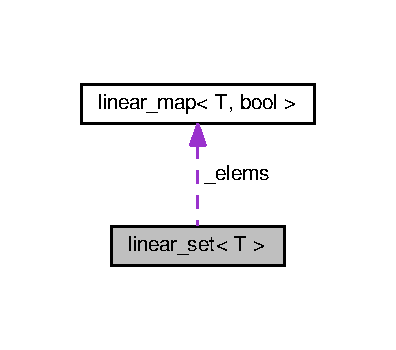
\includegraphics[width=190pt]{classlinear__set__coll__graph}
\end{center}
\end{figure}
\subsection*{Clases}
\begin{DoxyCompactItemize}
\item 
class \hyperlink{classlinear__set_1_1const__iterator}{const\-\_\-iterator}
\item 
class \hyperlink{classlinear__set_1_1iterator}{iterator}
\end{DoxyCompactItemize}
\subsection*{Tipos públicos}
\begin{DoxyCompactItemize}
\item 
\hypertarget{classlinear__set_a3d7088f5ad3d506bc94ad0fa62c40fed}{using {\bfseries value\-\_\-type} = T}\label{classlinear__set_a3d7088f5ad3d506bc94ad0fa62c40fed}

\item 
\hypertarget{classlinear__set_a502855ac3cffe6a33ba8eed857bd14bf}{using {\bfseries size\-\_\-type} = size\-\_\-t}\label{classlinear__set_a502855ac3cffe6a33ba8eed857bd14bf}

\end{DoxyCompactItemize}
\subsection*{Métodos públicos}
\begin{DoxyCompactItemize}
\item 
\hyperlink{classlinear__set_a6d872f648b8f79012ad962ad852f8ae7}{linear\-\_\-set} ()
\begin{DoxyCompactList}\small\item\em Crea un conjunto vacio. \end{DoxyCompactList}\item 
\hyperlink{classlinear__set_aa99e56c1ec649af8f0fa8c681d31fcb6}{linear\-\_\-set} (std\-::initializer\-\_\-list$<$ value\-\_\-type $>$ init)
\begin{DoxyCompactList}\small\item\em Crea un conjunto con los valores parámetros. \end{DoxyCompactList}\item 
{\footnotesize template$<$class Input\-It $>$ }\\\hyperlink{classlinear__set_ac1949a93e1927b46604fbdcecb8a1ae3}{linear\-\_\-set} (Input\-It first, Input\-It last)
\begin{DoxyCompactList}\small\item\em Crea un conjunto con los valores parámetros. \end{DoxyCompactList}\item 
\hyperlink{classlinear__set_a45f6e9a11657e0945e88300da619af22}{linear\-\_\-set} (const \hyperlink{classlinear__set}{linear\-\_\-set}$<$ T $>$ \&other)
\begin{DoxyCompactList}\small\item\em Constructor por copia. \end{DoxyCompactList}\item 
pair$<$ \hyperlink{classlinear__set_1_1iterator}{iterator}, bool $>$ \hyperlink{classlinear__set_a66b2d1323a28dcd2dd7511e4b65f4529}{insert} (const T \&x)
\begin{DoxyCompactList}\small\item\em Agrega el elemento al conjunto. \end{DoxyCompactList}\item 
\hyperlink{classlinear__set_1_1iterator}{iterator} \hyperlink{classlinear__set_a095fc4a1f15f43650efa7518aa58579f}{fast\-\_\-insert} (const value\-\_\-type \&v)
\begin{DoxyCompactList}\small\item\em Agrega el elemento al conjunto. \end{DoxyCompactList}\item 
size\-\_\-type \hyperlink{classlinear__set_a2199271b0b692ca35bfe4f5ee69b300a}{count} (const T \&x) const 
\begin{DoxyCompactList}\small\item\em Cantidad de apariciones del valor. \end{DoxyCompactList}\item 
bool \hyperlink{classlinear__set_ad1ebf082279d7992e12b434d52cf2338}{empty} () const 
\begin{DoxyCompactList}\small\item\em True si el conjunto está vacío. \end{DoxyCompactList}\item 
size\-\_\-type \hyperlink{classlinear__set_a48c78a9f6814516482724214d685540e}{size} () const 
\begin{DoxyCompactList}\small\item\em Tamaño del conjunto. \end{DoxyCompactList}\item 
size\-\_\-type \hyperlink{classlinear__set_a264d97735943af5490e73e469c3e7303}{erase} (const T \&x)
\begin{DoxyCompactList}\small\item\em Elimina el valor del conjunto. Devuelve la cantidad de elementos elminados. \end{DoxyCompactList}\item 
\hyperlink{classlinear__set_1_1iterator}{iterator} \hyperlink{classlinear__set_a415e0c8461f6a702129b7612a538ffb1}{find} (const T \&x)
\begin{DoxyCompactList}\small\item\em Devuelve un iterador relacionado al valor buscado. End si no está definida. \end{DoxyCompactList}\item 
\hyperlink{classlinear__set}{linear\-\_\-set}$<$ T $>$ \& \hyperlink{classlinear__set_a5bea24f94c4ea45550ec4b066ffb8cf1}{operator=} (const \hyperlink{classlinear__set}{linear\-\_\-set}$<$ T $>$ \&other)
\begin{DoxyCompactList}\small\item\em Operador asignación del conjunto. \end{DoxyCompactList}\item 
bool \hyperlink{classlinear__set_a519aaf53184baa0fb250dc13031c1c52}{operator==} (const \hyperlink{classlinear__set}{linear\-\_\-set}$<$ T $>$ \&other) const 
\begin{DoxyCompactList}\small\item\em True si los conjuntos son iguales. \end{DoxyCompactList}\item 
\hyperlink{classlinear__set_1_1iterator}{iterator} \hyperlink{classlinear__set_a80bad302b65a43aba2a0fbf5e4637a59}{begin} ()
\begin{DoxyCompactList}\small\item\em Devuelve un iterador al inicio del conjunto. \end{DoxyCompactList}\item 
\hyperlink{classlinear__set_1_1iterator}{iterator} \hyperlink{classlinear__set_aa16e2607ba7bc80c86eda9f2301d194d}{end} ()
\begin{DoxyCompactList}\small\item\em Devuelve un iterador a la posición pasando-\/el-\/último. \end{DoxyCompactList}\item 
\hyperlink{classlinear__set_1_1const__iterator}{const\-\_\-iterator} \hyperlink{classlinear__set_a618bae1c12e9bb0aa0f4f878dbafbdb5}{begin} () const 
\begin{DoxyCompactList}\small\item\em Devuelve un iterador const al inicio del conjunto. \end{DoxyCompactList}\item 
\hyperlink{classlinear__set_1_1const__iterator}{const\-\_\-iterator} \hyperlink{classlinear__set_a9cbffd97e4a2d8d89afdf81fab83dbaa}{end} () const 
\begin{DoxyCompactList}\small\item\em Devuelve un iterador const a la posición pasando-\/el-\/último. \end{DoxyCompactList}\end{DoxyCompactItemize}
\subsection*{Atributos privados}
\begin{Indent}{\bf Representación\-:}\par
{\em rep\-: \hyperlink{classlinear__set}{linear\-\_\-set(\-T)} $\to$ bool\par
rep(c) $\equiv$
\begin{DoxyItemize}
\item $\forall$ (t \-: T) (def?(t, \-\_\-elems) $\Rightarrow$ obtener(t, \-\_\-elems))
\end{DoxyItemize}

abs\-: \hyperlink{classlinear__set}{linear\-\_\-set(\-T)} $\to$ Conj(\-T)\par
abs(c) $\equiv$ c' $|$
\begin{DoxyItemize}
\item $\forall$ (x \-: T) x $\in$ c' $\Leftrightarrow$ def?(c, c) 
\end{DoxyItemize}}\begin{DoxyCompactItemize}
\item 
\hypertarget{classlinear__set_ab9ee1d2a9a2b2786152f68bd0039d201}{\hyperlink{classlinear__map}{linear\-\_\-map}$<$ T, bool $>$ {\bfseries \-\_\-elems}}\label{classlinear__set_ab9ee1d2a9a2b2786152f68bd0039d201}

\end{DoxyCompactItemize}
\end{Indent}


\subsection{Descripción detallada}
\subsubsection*{template$<$typename T$>$class linear\-\_\-set$<$ T $>$}

Conjunto con inserción en tiempo constante. 


\begin{DoxyTemplParams}{Template Parameters}
{\em T} & tipo paramétrico del conjunto Debe tener\-:
\begin{DoxyItemize}
\item operator==
\item Constructor por copia
\end{DoxyItemize}\\
\hline
\end{DoxyTemplParams}
{\bfseries se explica con} T\-A\-D Conjunto(\-T) 

\subsection{Documentación del constructor y destructor}
\hypertarget{classlinear__set_a6d872f648b8f79012ad962ad852f8ae7}{\index{linear\-\_\-set@{linear\-\_\-set}!linear\-\_\-set@{linear\-\_\-set}}
\index{linear\-\_\-set@{linear\-\_\-set}!linear_set@{linear\-\_\-set}}
\subsubsection[{linear\-\_\-set}]{\setlength{\rightskip}{0pt plus 5cm}template$<$class T $>$ {\bf linear\-\_\-set}$<$ T $>$\-::{\bf linear\-\_\-set} (
\begin{DoxyParamCaption}
{}
\end{DoxyParamCaption}
)}}\label{classlinear__set_a6d872f648b8f79012ad962ad852f8ae7}


Crea un conjunto vacio. 

\begin{DoxyPrecond}{Precondición}
true 
\end{DoxyPrecond}
\begin{DoxyPostcond}{Postcondición}
{\bfseries this} = $\emptyset$
\end{DoxyPostcond}

\begin{DoxyDescription}
\item[Complejidad Temporal]$O$(1)
\end{DoxyDescription}\hypertarget{classlinear__set_aa99e56c1ec649af8f0fa8c681d31fcb6}{\index{linear\-\_\-set@{linear\-\_\-set}!linear\-\_\-set@{linear\-\_\-set}}
\index{linear\-\_\-set@{linear\-\_\-set}!linear_set@{linear\-\_\-set}}
\subsubsection[{linear\-\_\-set}]{\setlength{\rightskip}{0pt plus 5cm}template$<$class T $>$ {\bf linear\-\_\-set}$<$ T $>$\-::{\bf linear\-\_\-set} (
\begin{DoxyParamCaption}
\item[{std\-::initializer\-\_\-list$<$ value\-\_\-type $>$}]{init}
\end{DoxyParamCaption}
)}}\label{classlinear__set_aa99e56c1ec649af8f0fa8c681d31fcb6}


Crea un conjunto con los valores parámetros. 

\begin{DoxyPrecond}{Precondición}
true 
\end{DoxyPrecond}
\begin{DoxyPostcond}{Postcondición}
( $\forall$ x \-: T) x $\in$ {\bfseries this} $\Leftrightarrow$ está?(x, init)
\end{DoxyPostcond}

\begin{DoxyDescription}
\item[Complejidad Temporal]$O$(long(init) $\ast$ copy(\-T))
\end{DoxyDescription}\hypertarget{classlinear__set_ac1949a93e1927b46604fbdcecb8a1ae3}{\index{linear\-\_\-set@{linear\-\_\-set}!linear\-\_\-set@{linear\-\_\-set}}
\index{linear\-\_\-set@{linear\-\_\-set}!linear_set@{linear\-\_\-set}}
\subsubsection[{linear\-\_\-set}]{\setlength{\rightskip}{0pt plus 5cm}template$<$class T $>$ template$<$class Input\-It $>$ {\bf linear\-\_\-set}$<$ T $>$\-::{\bf linear\-\_\-set} (
\begin{DoxyParamCaption}
\item[{Input\-It}]{first, }
\item[{Input\-It}]{last}
\end{DoxyParamCaption}
)}}\label{classlinear__set_ac1949a93e1927b46604fbdcecb8a1ae3}


Crea un conjunto con los valores parámetros. 

\begin{DoxyPrecond}{Precondición}
first y last son iteradores del mismo contenedor 
\end{DoxyPrecond}
\begin{DoxyPostcond}{Postcondición}
{\bfseries this} tiene solo los valores en el rango first -\/$>$ last
\end{DoxyPostcond}

\begin{DoxyDescription}
\item[Complejidad Temporal]$O$($\vert$last -\/ first$\vert$ $\ast$ copy(\-T))
\end{DoxyDescription}\hypertarget{classlinear__set_a45f6e9a11657e0945e88300da619af22}{\index{linear\-\_\-set@{linear\-\_\-set}!linear\-\_\-set@{linear\-\_\-set}}
\index{linear\-\_\-set@{linear\-\_\-set}!linear_set@{linear\-\_\-set}}
\subsubsection[{linear\-\_\-set}]{\setlength{\rightskip}{0pt plus 5cm}template$<$class T$>$ {\bf linear\-\_\-set}$<$ T $>$\-::{\bf linear\-\_\-set} (
\begin{DoxyParamCaption}
\item[{const {\bf linear\-\_\-set}$<$ T $>$ \&}]{other}
\end{DoxyParamCaption}
)}}\label{classlinear__set_a45f6e9a11657e0945e88300da619af22}


Constructor por copia. 

\begin{DoxyPrecond}{Precondición}
true 
\end{DoxyPrecond}
\begin{DoxyPostcond}{Postcondición}
{\bfseries this} es una copia de other. No hay aliasing.
\end{DoxyPostcond}

\begin{DoxyDescription}
\item[Complejidad Temporal]$O$(\#(other) $\ast$ copy(\-T))
\end{DoxyDescription}

\subsection{Documentación de las funciones miembro}
\hypertarget{classlinear__set_a80bad302b65a43aba2a0fbf5e4637a59}{\index{linear\-\_\-set@{linear\-\_\-set}!begin@{begin}}
\index{begin@{begin}!linear_set@{linear\-\_\-set}}
\subsubsection[{begin}]{\setlength{\rightskip}{0pt plus 5cm}template$<$class T $>$ {\bf linear\-\_\-set}$<$ T $>$\-::{\bf iterator} {\bf linear\-\_\-set}$<$ T $>$\-::begin (
\begin{DoxyParamCaption}
{}
\end{DoxyParamCaption}
)}}\label{classlinear__set_a80bad302b65a43aba2a0fbf5e4637a59}


Devuelve un iterador al inicio del conjunto. 

\begin{DoxyPrecond}{Precondición}
true 
\end{DoxyPrecond}
\begin{DoxyPostcond}{Postcondición}
{\bfseries res} apunta al inicio del conjunto
\end{DoxyPostcond}

\begin{DoxyDescription}
\item[Complejidad Temporal]$O$(1)
\end{DoxyDescription}\hypertarget{classlinear__set_a618bae1c12e9bb0aa0f4f878dbafbdb5}{\index{linear\-\_\-set@{linear\-\_\-set}!begin@{begin}}
\index{begin@{begin}!linear_set@{linear\-\_\-set}}
\subsubsection[{begin}]{\setlength{\rightskip}{0pt plus 5cm}template$<$class T $>$ {\bf linear\-\_\-set}$<$ T $>$\-::{\bf const\-\_\-iterator} {\bf linear\-\_\-set}$<$ T $>$\-::begin (
\begin{DoxyParamCaption}
{}
\end{DoxyParamCaption}
) const}}\label{classlinear__set_a618bae1c12e9bb0aa0f4f878dbafbdb5}


Devuelve un iterador const al inicio del conjunto. 

\begin{DoxyPrecond}{Precondición}
true 
\end{DoxyPrecond}
\begin{DoxyPostcond}{Postcondición}
{\bfseries res} apunta al inicio del conjunto
\end{DoxyPostcond}

\begin{DoxyDescription}
\item[Complejidad Temporal]$O$(1)
\end{DoxyDescription}\hypertarget{classlinear__set_a2199271b0b692ca35bfe4f5ee69b300a}{\index{linear\-\_\-set@{linear\-\_\-set}!count@{count}}
\index{count@{count}!linear_set@{linear\-\_\-set}}
\subsubsection[{count}]{\setlength{\rightskip}{0pt plus 5cm}template$<$class T$>$ {\bf linear\-\_\-set}$<$ T $>$\-::size\-\_\-type {\bf linear\-\_\-set}$<$ T $>$\-::count (
\begin{DoxyParamCaption}
\item[{const T \&}]{x}
\end{DoxyParamCaption}
) const}}\label{classlinear__set_a2199271b0b692ca35bfe4f5ee69b300a}


Cantidad de apariciones del valor. 

\begin{DoxyPrecond}{Precondición}
true 
\end{DoxyPrecond}
\begin{DoxyPostcond}{Postcondición}
(x $\in$ {\bfseries this} $\land$ {\bfseries res} = 1) $\lor$ (x  $\in$ {\bfseries this} $\land$ {\bfseries res} = 0)
\end{DoxyPostcond}

\begin{DoxyDescription}
\item[Complejidad Temporal]$O$(n $\ast$ cmp(\-T))
\end{DoxyDescription}\hypertarget{classlinear__set_ad1ebf082279d7992e12b434d52cf2338}{\index{linear\-\_\-set@{linear\-\_\-set}!empty@{empty}}
\index{empty@{empty}!linear_set@{linear\-\_\-set}}
\subsubsection[{empty}]{\setlength{\rightskip}{0pt plus 5cm}template$<$class T $>$ bool {\bf linear\-\_\-set}$<$ T $>$\-::empty (
\begin{DoxyParamCaption}
{}
\end{DoxyParamCaption}
) const}}\label{classlinear__set_ad1ebf082279d7992e12b434d52cf2338}


True si el conjunto está vacío. 

\begin{DoxyPrecond}{Precondición}
true 
\end{DoxyPrecond}
\begin{DoxyPostcond}{Postcondición}
{\bfseries res} = $\emptyset$?({\bfseries this})
\end{DoxyPostcond}

\begin{DoxyDescription}
\item[Complejidad Temporal]$O$(1)
\end{DoxyDescription}\hypertarget{classlinear__set_aa16e2607ba7bc80c86eda9f2301d194d}{\index{linear\-\_\-set@{linear\-\_\-set}!end@{end}}
\index{end@{end}!linear_set@{linear\-\_\-set}}
\subsubsection[{end}]{\setlength{\rightskip}{0pt plus 5cm}template$<$class T $>$ {\bf linear\-\_\-set}$<$ T $>$\-::{\bf iterator} {\bf linear\-\_\-set}$<$ T $>$\-::end (
\begin{DoxyParamCaption}
{}
\end{DoxyParamCaption}
)}}\label{classlinear__set_aa16e2607ba7bc80c86eda9f2301d194d}


Devuelve un iterador a la posición pasando-\/el-\/último. 

\begin{DoxyPrecond}{Precondición}
true 
\end{DoxyPrecond}
\begin{DoxyPostcond}{Postcondición}
{\bfseries res} apunta a la posición pasando-\/el-\/último
\end{DoxyPostcond}

\begin{DoxyDescription}
\item[Complejidad Temporal]$O$(1)
\end{DoxyDescription}\hypertarget{classlinear__set_a9cbffd97e4a2d8d89afdf81fab83dbaa}{\index{linear\-\_\-set@{linear\-\_\-set}!end@{end}}
\index{end@{end}!linear_set@{linear\-\_\-set}}
\subsubsection[{end}]{\setlength{\rightskip}{0pt plus 5cm}template$<$class T $>$ {\bf linear\-\_\-set}$<$ T $>$\-::{\bf const\-\_\-iterator} {\bf linear\-\_\-set}$<$ T $>$\-::end (
\begin{DoxyParamCaption}
{}
\end{DoxyParamCaption}
) const}}\label{classlinear__set_a9cbffd97e4a2d8d89afdf81fab83dbaa}


Devuelve un iterador const a la posición pasando-\/el-\/último. 

\begin{DoxyPrecond}{Precondición}
true 
\end{DoxyPrecond}
\begin{DoxyPostcond}{Postcondición}
{\bfseries res} apunta a la posición pasando-\/el-\/último
\end{DoxyPostcond}

\begin{DoxyDescription}
\item[Complejidad Temporal]$O$(1)
\end{DoxyDescription}\hypertarget{classlinear__set_a264d97735943af5490e73e469c3e7303}{\index{linear\-\_\-set@{linear\-\_\-set}!erase@{erase}}
\index{erase@{erase}!linear_set@{linear\-\_\-set}}
\subsubsection[{erase}]{\setlength{\rightskip}{0pt plus 5cm}template$<$class T$>$ {\bf linear\-\_\-set}$<$ T $>$\-::size\-\_\-type {\bf linear\-\_\-set}$<$ T $>$\-::erase (
\begin{DoxyParamCaption}
\item[{const T \&}]{x}
\end{DoxyParamCaption}
)}}\label{classlinear__set_a264d97735943af5490e73e469c3e7303}


Elimina el valor del conjunto. Devuelve la cantidad de elementos elminados. 

\begin{DoxyPrecond}{Precondición}
c == {\bfseries this} $\land$ x $\in$ {\bfseries this} 
\end{DoxyPrecond}
\begin{DoxyPostcond}{Postcondición}
{\bfseries this} == c -\/ \{x\} $\land$ {\bfseries res} = 1
\end{DoxyPostcond}

\begin{DoxyDescription}
\item[Complejidad Temporal]$O$(\#claves({\bfseries this}))
\end{DoxyDescription}\hypertarget{classlinear__set_a095fc4a1f15f43650efa7518aa58579f}{\index{linear\-\_\-set@{linear\-\_\-set}!fast\-\_\-insert@{fast\-\_\-insert}}
\index{fast\-\_\-insert@{fast\-\_\-insert}!linear_set@{linear\-\_\-set}}
\subsubsection[{fast\-\_\-insert}]{\setlength{\rightskip}{0pt plus 5cm}template$<$typename T$>$ {\bf linear\-\_\-set}$<$ T $>$\-::{\bf iterator} {\bf linear\-\_\-set}$<$ T $>$\-::fast\-\_\-insert (
\begin{DoxyParamCaption}
\item[{const value\-\_\-type \&}]{v}
\end{DoxyParamCaption}
)}}\label{classlinear__set_a095fc4a1f15f43650efa7518aa58579f}


Agrega el elemento al conjunto. 

\begin{DoxyPrecond}{Precondición}
c = {\bfseries this} $\land$ $\lnot$ x $\in$ {\bfseries this} 
\end{DoxyPrecond}
\begin{DoxyPostcond}{Postcondición}
{\bfseries this} = Ag(x, c) y {\bfseries res} apunta al elemento agregado.
\end{DoxyPostcond}

\begin{DoxyDescription}
\item[Complejidad Temporal]$O$(copy(v))
\end{DoxyDescription}\hypertarget{classlinear__set_a415e0c8461f6a702129b7612a538ffb1}{\index{linear\-\_\-set@{linear\-\_\-set}!find@{find}}
\index{find@{find}!linear_set@{linear\-\_\-set}}
\subsubsection[{find}]{\setlength{\rightskip}{0pt plus 5cm}template$<$class T$>$ {\bf linear\-\_\-set}$<$ T $>$\-::{\bf iterator} {\bf linear\-\_\-set}$<$ T $>$\-::find (
\begin{DoxyParamCaption}
\item[{const T \&}]{x}
\end{DoxyParamCaption}
)}}\label{classlinear__set_a415e0c8461f6a702129b7612a538ffb1}


Devuelve un iterador relacionado al valor buscado. End si no está definida. 

\begin{DoxyPrecond}{Precondición}
true 
\end{DoxyPrecond}
\begin{DoxyPostcond}{Postcondición}

\begin{DoxyItemize}
\item x $\in$ {\bfseries this} $\Rightarrow$ {\bfseries res} apunta a la aparición de x en el conjunto
\item x $\in$ {\bfseries this} $\Rightarrow$ {\bfseries res} es end
\end{DoxyItemize}
\end{DoxyPostcond}

\begin{DoxyDescription}
\item[Complejidad Temporal]$O$(\#claves({\bfseries this}))
\end{DoxyDescription}\hypertarget{classlinear__set_a66b2d1323a28dcd2dd7511e4b65f4529}{\index{linear\-\_\-set@{linear\-\_\-set}!insert@{insert}}
\index{insert@{insert}!linear_set@{linear\-\_\-set}}
\subsubsection[{insert}]{\setlength{\rightskip}{0pt plus 5cm}template$<$class T$>$ pair$<$ typename {\bf linear\-\_\-set}$<$ T $>$\-::{\bf iterator}, bool $>$ {\bf linear\-\_\-set}$<$ T $>$\-::insert (
\begin{DoxyParamCaption}
\item[{const T \&}]{x}
\end{DoxyParamCaption}
)}}\label{classlinear__set_a66b2d1323a28dcd2dd7511e4b65f4529}


Agrega el elemento al conjunto. 

El elemento no se agrega si ya estaba.

\begin{DoxyPrecond}{Precondición}
c = {\bfseries this} 
\end{DoxyPrecond}
\begin{DoxyPostcond}{Postcondición}
{\bfseries this} = Ag(x, c) y $\pi_1$({\bfseries res}) apunta al elemento agregado y $\pi_2$({\bfseries res}) es true si x no estaba ya en el conjunto.
\end{DoxyPostcond}

\begin{DoxyDescription}
\item[Complejidad Temporal]$O$(\#claves({\bfseries this}) + copy(v))
\end{DoxyDescription}\hypertarget{classlinear__set_a5bea24f94c4ea45550ec4b066ffb8cf1}{\index{linear\-\_\-set@{linear\-\_\-set}!operator=@{operator=}}
\index{operator=@{operator=}!linear_set@{linear\-\_\-set}}
\subsubsection[{operator=}]{\setlength{\rightskip}{0pt plus 5cm}template$<$class T$>$ {\bf linear\-\_\-set}$<$ T $>$ \& {\bf linear\-\_\-set}$<$ T $>$\-::operator= (
\begin{DoxyParamCaption}
\item[{const {\bf linear\-\_\-set}$<$ T $>$ \&}]{other}
\end{DoxyParamCaption}
)}}\label{classlinear__set_a5bea24f94c4ea45550ec4b066ffb8cf1}


Operador asignación del conjunto. 

\begin{DoxyPrecond}{Precondición}
true 
\end{DoxyPrecond}
\begin{DoxyPostcond}{Postcondición}
{\bfseries this} == other y {\bfseries res} refiere a {\bfseries this}
\end{DoxyPostcond}

\begin{DoxyDescription}
\item[Complejidad Temporal]$O$(\#claves({\bfseries this}) + \#(other) $\ast$ copy(\-T))
\end{DoxyDescription}\hypertarget{classlinear__set_a519aaf53184baa0fb250dc13031c1c52}{\index{linear\-\_\-set@{linear\-\_\-set}!operator==@{operator==}}
\index{operator==@{operator==}!linear_set@{linear\-\_\-set}}
\subsubsection[{operator==}]{\setlength{\rightskip}{0pt plus 5cm}template$<$class T$>$ bool {\bf linear\-\_\-set}$<$ T $>$\-::operator== (
\begin{DoxyParamCaption}
\item[{const {\bf linear\-\_\-set}$<$ T $>$ \&}]{other}
\end{DoxyParamCaption}
) const}}\label{classlinear__set_a519aaf53184baa0fb250dc13031c1c52}


True si los conjuntos son iguales. 


\begin{DoxyDescription}
\item[Complejidad Temporal]$O$(\#({\bfseries this}) $\ast$ \#(other))
\end{DoxyDescription}\hypertarget{classlinear__set_a48c78a9f6814516482724214d685540e}{\index{linear\-\_\-set@{linear\-\_\-set}!size@{size}}
\index{size@{size}!linear_set@{linear\-\_\-set}}
\subsubsection[{size}]{\setlength{\rightskip}{0pt plus 5cm}template$<$class T $>$ {\bf linear\-\_\-set}$<$ T $>$\-::size\-\_\-type {\bf linear\-\_\-set}$<$ T $>$\-::size (
\begin{DoxyParamCaption}
{}
\end{DoxyParamCaption}
) const}}\label{classlinear__set_a48c78a9f6814516482724214d685540e}


Tamaño del conjunto. 

\begin{DoxyPrecond}{Precondición}
true 
\end{DoxyPrecond}
\begin{DoxyPostcond}{Postcondición}
{\bfseries res} = \#clave({\bfseries this})
\end{DoxyPostcond}

\begin{DoxyDescription}
\item[Complejidad Temporal]$O$(1)
\end{DoxyDescription}

La documentación para esta clase fue generada a partir de los siguientes ficheros\-:\begin{DoxyCompactItemize}
\item 
src/linear\-\_\-set.\-h\item 
src/linear\-\_\-set.\-hpp\end{DoxyCompactItemize}

\hypertarget{structstring__map_1_1Nodo}{\section{Referencia de la Estructura string\-\_\-map$<$ T $>$\-:\-:Nodo}
\label{structstring__map_1_1Nodo}\index{string\-\_\-map$<$ T $>$\-::\-Nodo@{string\-\_\-map$<$ T $>$\-::\-Nodo}}
}


Diagrama de colaboración para string\-\_\-map$<$ T $>$\-:\-:Nodo\-:
\nopagebreak
\begin{figure}[H]
\begin{center}
\leavevmode
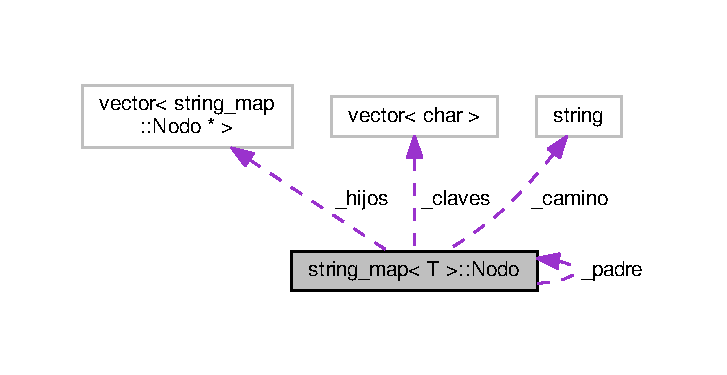
\includegraphics[width=349pt]{structstring__map_1_1Nodo__coll__graph}
\end{center}
\end{figure}
\subsection*{Métodos públicos}
\begin{DoxyCompactItemize}
\item 
\hypertarget{structstring__map_1_1Nodo_a8ac594cdba5810ff914ffc4efc63550e}{{\bfseries Nodo} (bool definido, const string camino, T \&obtener, \hyperlink{structstring__map_1_1Nodo}{Nodo} $\ast$padre, int pos\-En\-Padre)}\label{structstring__map_1_1Nodo_a8ac594cdba5810ff914ffc4efc63550e}

\end{DoxyCompactItemize}
\subsection*{Atributos públicos}
\begin{DoxyCompactItemize}
\item 
\hypertarget{structstring__map_1_1Nodo_a793784e5c0c9713764ef4023ad58f8d9}{vector$<$ char $>$ {\bfseries \-\_\-claves}}\label{structstring__map_1_1Nodo_a793784e5c0c9713764ef4023ad58f8d9}

\item 
\hypertarget{structstring__map_1_1Nodo_ae2d98d22f3bcb8dbb5ed114ba8603328}{vector$<$ \hyperlink{structstring__map_1_1Nodo}{Nodo} $\ast$ $>$ {\bfseries \-\_\-hijos}}\label{structstring__map_1_1Nodo_ae2d98d22f3bcb8dbb5ed114ba8603328}

\item 
\hypertarget{structstring__map_1_1Nodo_ab1ba84d07c625f2120ff58563edcaa0d}{T $\ast$ {\bfseries \-\_\-obtener}}\label{structstring__map_1_1Nodo_ab1ba84d07c625f2120ff58563edcaa0d}

\item 
\hypertarget{structstring__map_1_1Nodo_a62d242d0582019e18965463eaa1db910}{\hyperlink{structstring__map_1_1Nodo}{Nodo} $\ast$ {\bfseries \-\_\-padre}}\label{structstring__map_1_1Nodo_a62d242d0582019e18965463eaa1db910}

\item 
\hypertarget{structstring__map_1_1Nodo_a2f4d32924b849d2d366c25485ad1c072}{string $\ast$ {\bfseries \-\_\-camino}}\label{structstring__map_1_1Nodo_a2f4d32924b849d2d366c25485ad1c072}

\item 
\hypertarget{structstring__map_1_1Nodo_a0d081617ab62571ddceaffe4a8ea9f38}{bool {\bfseries \-\_\-definido}}\label{structstring__map_1_1Nodo_a0d081617ab62571ddceaffe4a8ea9f38}

\item 
\hypertarget{structstring__map_1_1Nodo_afc927f58dc591a437293d31ebdffa084}{int {\bfseries \-\_\-pos\-En\-Padre}}\label{structstring__map_1_1Nodo_afc927f58dc591a437293d31ebdffa084}

\item 
\hypertarget{structstring__map_1_1Nodo_a9fcf013757b89c9d9670195a4f76bc95}{value\-\_\-type $\ast$ {\bfseries v}}\label{structstring__map_1_1Nodo_a9fcf013757b89c9d9670195a4f76bc95}

\end{DoxyCompactItemize}


La documentación para esta estructura fue generada a partir del siguiente fichero\-:\begin{DoxyCompactItemize}
\item 
src/string\-\_\-map.\-h\end{DoxyCompactItemize}

\hypertarget{classRegistro}{\section{Referencia de la Clase Registro}
\label{classRegistro}\index{Registro@{Registro}}
}


Representa un registro de una tabla.  




{\ttfamily \#include $<$Registro.\-h$>$}



Diagrama de colaboración para Registro\-:\nopagebreak
\begin{figure}[H]
\begin{center}
\leavevmode
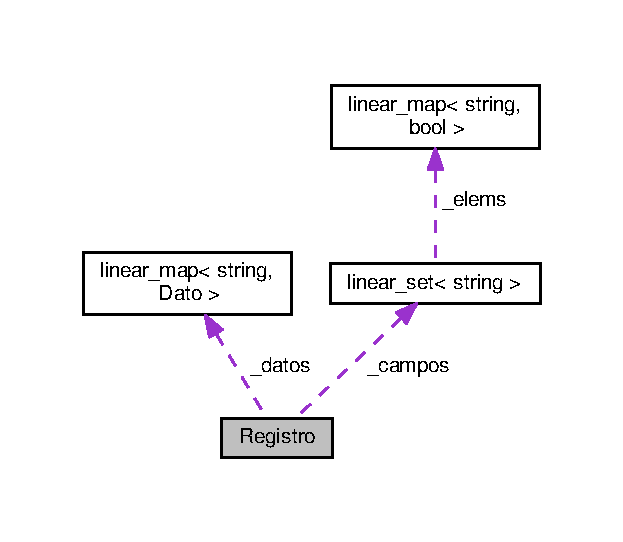
\includegraphics[width=299pt]{classRegistro__coll__graph}
\end{center}
\end{figure}
\subsection*{Métodos públicos}
\begin{DoxyCompactItemize}
\item 
\hyperlink{classRegistro_af3717314d0e658a463ffd8ac5b073441}{Registro} (const vector$<$ string $>$ \&\hyperlink{classRegistro_af082664a69c70eb5d29dcad6522242fc}{campos}, const vector$<$ \hyperlink{classDato}{Dato} $>$ \&datos)
\begin{DoxyCompactList}\small\item\em Genera un nuevo registro con los campos y valores designados. \end{DoxyCompactList}\item 
const \hyperlink{classDato}{Dato} \& \hyperlink{classRegistro_a5191c0af2f375525601819cfbb477287}{dato} (const string \&campo) const 
\begin{DoxyCompactList}\small\item\em Devuelve el dato asociado a un campo. \end{DoxyCompactList}\item 
const \hyperlink{classlinear__set}{linear\-\_\-set}$<$ string $>$ \& \hyperlink{classRegistro_af082664a69c70eb5d29dcad6522242fc}{campos} () const 
\begin{DoxyCompactList}\small\item\em Devuelve los campos definidos en un registro. \end{DoxyCompactList}\end{DoxyCompactItemize}
\subsection*{Atributos privados}
\begin{Indent}{\bf Representación}\par
{\em rep\-: registro $\to$ bool\par
rep(d) $\equiv$
\begin{DoxyItemize}
\item \-\_\-campos = claves(\-\_\-datos)
\end{DoxyItemize}

abs\-: registro $\to$ \hyperlink{classRegistro}{Registro}\par
abs(r) $\equiv$ r' $|$
\begin{DoxyItemize}
\item campos(r') = \-\_\-campos $\land$
\item $\forall$ (c \-: string) c  \-\_\-campos $\Rightarrow$ valor(c, r') = valor(c, \-\_\-datos) 
\end{DoxyItemize}}\begin{DoxyCompactItemize}
\item 
\hypertarget{classRegistro_ad6c12d81cb20086a4642f4b85fe8063b}{\hyperlink{classlinear__set}{linear\-\_\-set}$<$ string $>$ {\bfseries \-\_\-campos}}\label{classRegistro_ad6c12d81cb20086a4642f4b85fe8063b}

\item 
\hypertarget{classRegistro_a87c21ec5101090321cef177f3a256132}{\hyperlink{classlinear__map}{linear\-\_\-map}$<$ string, \hyperlink{classDato}{Dato} $>$ {\bfseries \-\_\-datos}}\label{classRegistro_a87c21ec5101090321cef177f3a256132}

\end{DoxyCompactItemize}
\end{Indent}
\subsection*{Amigas}
\begin{DoxyCompactItemize}
\item 
\hypertarget{classRegistro_a66788288d92ef16b5a3aab86ae6d87fc}{ostream \& {\bfseries operator$<$$<$} (ostream \&, const \hyperlink{classRegistro}{Registro} \&)}\label{classRegistro_a66788288d92ef16b5a3aab86ae6d87fc}

\end{DoxyCompactItemize}


\subsection{Descripción detallada}
Representa un registro de una tabla. 

Un registro asocia campos identificados con un string con valores específicos.

{\bfseries se explica con} T\-A\-D Diccionario(string, Dato) 

\subsection{Documentación del constructor y destructor}
\hypertarget{classRegistro_af3717314d0e658a463ffd8ac5b073441}{\index{Registro@{Registro}!Registro@{Registro}}
\index{Registro@{Registro}!Registro@{Registro}}
\subsubsection[{Registro}]{\setlength{\rightskip}{0pt plus 5cm}Registro\-::\-Registro (
\begin{DoxyParamCaption}
\item[{const vector$<$ string $>$ \&}]{campos, }
\item[{const vector$<$ {\bf Dato} $>$ \&}]{datos}
\end{DoxyParamCaption}
)}}\label{classRegistro_af3717314d0e658a463ffd8ac5b073441}


Genera un nuevo registro con los campos y valores designados. 

\begin{DoxyPrecond}{Precondición}
long(campos) = long(datos) 
\end{DoxyPrecond}
\begin{DoxyPostcond}{Postcondición}
{\bfseries res} = nuevo\-Registro(campos, datos)
\end{DoxyPostcond}

\begin{DoxyDescription}
\item[Complejidad Temporal]$O$(long(campos) $\ast$ (copy(campo) + copy(dato)))
\end{DoxyDescription}

\subsection{Documentación de las funciones miembro}
\hypertarget{classRegistro_af082664a69c70eb5d29dcad6522242fc}{\index{Registro@{Registro}!campos@{campos}}
\index{campos@{campos}!Registro@{Registro}}
\subsubsection[{campos}]{\setlength{\rightskip}{0pt plus 5cm}const {\bf linear\-\_\-set}$<$ string $>$ \& Registro\-::campos (
\begin{DoxyParamCaption}
{}
\end{DoxyParamCaption}
) const}}\label{classRegistro_af082664a69c70eb5d29dcad6522242fc}


Devuelve los campos definidos en un registro. 

El conjunto de campos se devuelve por referencia

\begin{DoxyPrecond}{Precondición}
true 
\end{DoxyPrecond}
\begin{DoxyPostcond}{Postcondición}
{\bfseries res} = campos({\bfseries this})
\end{DoxyPostcond}

\begin{DoxyDescription}
\item[Complejidad Temporal]$O$(1)
\end{DoxyDescription}\hypertarget{classRegistro_a5191c0af2f375525601819cfbb477287}{\index{Registro@{Registro}!dato@{dato}}
\index{dato@{dato}!Registro@{Registro}}
\subsubsection[{dato}]{\setlength{\rightskip}{0pt plus 5cm}const {\bf Dato} \& Registro\-::dato (
\begin{DoxyParamCaption}
\item[{const string \&}]{campo}
\end{DoxyParamCaption}
) const}}\label{classRegistro_a5191c0af2f375525601819cfbb477287}


Devuelve el dato asociado a un campo. 

Devuelve el dato por referencia no modificable.

\begin{DoxyPrecond}{Precondición}
campo  campos({\bfseries this}) 
\end{DoxyPrecond}
\begin{DoxyPostcond}{Postcondición}
{\bfseries res} = valor(campo, {\bfseries this})
\end{DoxyPostcond}

\begin{DoxyDescription}
\item[Complejidad Temporal]$O$(long(campos({\bfseries this})) $\ast$ cmp(campo))
\end{DoxyDescription}

La documentación para esta clase fue generada a partir de los siguientes ficheros\-:\begin{DoxyCompactItemize}
\item 
src/Registro.\-h\item 
src/Registro.\-cpp\end{DoxyCompactItemize}

\hypertarget{classRestriccion}{\section{Referencia de la Clase Restriccion}
\label{classRestriccion}\index{Restriccion@{Restriccion}}
}


Representa una restricción de la base de datos.  




{\ttfamily \#include $<$Restriccion.\-h$>$}



Diagrama de colaboración para Restriccion\-:
\nopagebreak
\begin{figure}[H]
\begin{center}
\leavevmode
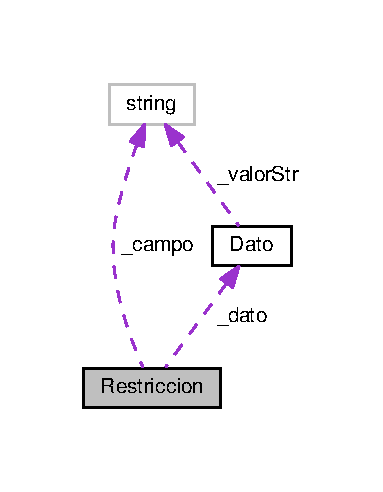
\includegraphics[width=184pt]{classRestriccion__coll__graph}
\end{center}
\end{figure}
\subsection*{Métodos públicos}
\begin{DoxyCompactItemize}
\item 
\hyperlink{classRestriccion_a6a2bb9363d1083319784caec16d9c47f}{Restriccion} (const string \&\hyperlink{classRestriccion_abee29e2435df3c0c2c8dd6330c7ad174}{campo}, const \hyperlink{classDato}{Dato} \&\hyperlink{classRestriccion_ac9b624d6ed5510aabb52ff68b77ce2f2}{dato}, bool \hyperlink{classRestriccion_ad1a9be4996f3ab4d9a26853c0b96f387}{igual})
\begin{DoxyCompactList}\small\item\em Constructor de Restricción. \end{DoxyCompactList}\item 
const string \& \hyperlink{classRestriccion_abee29e2435df3c0c2c8dd6330c7ad174}{campo} () const 
\begin{DoxyCompactList}\small\item\em Observador campo. \end{DoxyCompactList}\item 
const \hyperlink{classDato}{Dato} \& \hyperlink{classRestriccion_ac9b624d6ed5510aabb52ff68b77ce2f2}{dato} () const 
\begin{DoxyCompactList}\small\item\em Observador dato. \end{DoxyCompactList}\item 
const bool \& \hyperlink{classRestriccion_ad1a9be4996f3ab4d9a26853c0b96f387}{igual} () const 
\begin{DoxyCompactList}\small\item\em Observador por\-Igual. \end{DoxyCompactList}\end{DoxyCompactItemize}
\subsection*{Atributos privados}
\begin{Indent}{\bf Representación}\par
{\em rep\-: restricción $\to$ bool\par
rep(r) $\equiv$ true

abs\-: restricción $\to$ Restricción \par
abs(r) $\equiv$ r' $|$
\begin{DoxyItemize}
\item campo(r') = \-\_\-campo $\land$
\item dato(r') = \-\_\-dato $\land$
\item por\-Igual(r') = \-\_\-igual 
\end{DoxyItemize}}\begin{DoxyCompactItemize}
\item 
\hypertarget{classRestriccion_a30dff6c0b92a829c82905d01c034fdf4}{string {\bfseries \-\_\-campo}}\label{classRestriccion_a30dff6c0b92a829c82905d01c034fdf4}

\item 
\hypertarget{classRestriccion_a1052448653d6cb5f14537e432b20983c}{\hyperlink{classDato}{Dato} {\bfseries \-\_\-dato}}\label{classRestriccion_a1052448653d6cb5f14537e432b20983c}

\item 
\hypertarget{classRestriccion_ac7f162378d50128fc313c811ff40266b}{bool {\bfseries \-\_\-igual}}\label{classRestriccion_ac7f162378d50128fc313c811ff40266b}

\end{DoxyCompactItemize}
\end{Indent}


\subsection{Descripción detallada}
Representa una restricción de la base de datos. 

{\bfseries se explica con} T\-A\-D \hyperlink{classRestriccion}{Restriccion} 

\subsection{Documentación del constructor y destructor}
\hypertarget{classRestriccion_a6a2bb9363d1083319784caec16d9c47f}{\index{Restriccion@{Restriccion}!Restriccion@{Restriccion}}
\index{Restriccion@{Restriccion}!Restriccion@{Restriccion}}
\subsubsection[{Restriccion}]{\setlength{\rightskip}{0pt plus 5cm}Restriccion\-::\-Restriccion (
\begin{DoxyParamCaption}
\item[{const string \&}]{campo, }
\item[{const {\bf Dato} \&}]{dato, }
\item[{bool}]{igual}
\end{DoxyParamCaption}
)}}\label{classRestriccion_a6a2bb9363d1083319784caec16d9c47f}


Constructor de Restricción. 

\begin{DoxyPrecond}{Precondición}
true 
\end{DoxyPrecond}
\begin{DoxyPostcond}{Postcondición}
{\bfseries this} == nueva(campo, dato, igual)
\end{DoxyPostcond}

\begin{DoxyDescription}
\item[Complejidad Temporal]$O$(L)
\end{DoxyDescription}

\subsection{Documentación de las funciones miembro}
\hypertarget{classRestriccion_abee29e2435df3c0c2c8dd6330c7ad174}{\index{Restriccion@{Restriccion}!campo@{campo}}
\index{campo@{campo}!Restriccion@{Restriccion}}
\subsubsection[{campo}]{\setlength{\rightskip}{0pt plus 5cm}const string \& Restriccion\-::campo (
\begin{DoxyParamCaption}
{}
\end{DoxyParamCaption}
) const}}\label{classRestriccion_abee29e2435df3c0c2c8dd6330c7ad174}


Observador campo. 

El valor resultado se devuelve por referencia

\begin{DoxyPrecond}{Precondición}
true 
\end{DoxyPrecond}
\begin{DoxyPostcond}{Postcondición}
{\bfseries res} == campo({\bfseries this}\}
\end{DoxyPostcond}

\begin{DoxyDescription}
\item[Complejidad Temporal]$O$(1)
\end{DoxyDescription}\hypertarget{classRestriccion_ac9b624d6ed5510aabb52ff68b77ce2f2}{\index{Restriccion@{Restriccion}!dato@{dato}}
\index{dato@{dato}!Restriccion@{Restriccion}}
\subsubsection[{dato}]{\setlength{\rightskip}{0pt plus 5cm}const {\bf Dato} \& Restriccion\-::dato (
\begin{DoxyParamCaption}
{}
\end{DoxyParamCaption}
) const}}\label{classRestriccion_ac9b624d6ed5510aabb52ff68b77ce2f2}


Observador dato. 

El valor resultado se devuelve por referencia

\begin{DoxyPrecond}{Precondición}
true 
\end{DoxyPrecond}
\begin{DoxyPostcond}{Postcondición}
{\bfseries res} == dato({\bfseries this}\}
\end{DoxyPostcond}

\begin{DoxyDescription}
\item[Complejidad Temporal]$O$(1)
\end{DoxyDescription}\hypertarget{classRestriccion_ad1a9be4996f3ab4d9a26853c0b96f387}{\index{Restriccion@{Restriccion}!igual@{igual}}
\index{igual@{igual}!Restriccion@{Restriccion}}
\subsubsection[{igual}]{\setlength{\rightskip}{0pt plus 5cm}const bool \& Restriccion\-::igual (
\begin{DoxyParamCaption}
{}
\end{DoxyParamCaption}
) const}}\label{classRestriccion_ad1a9be4996f3ab4d9a26853c0b96f387}


Observador por\-Igual. 

El valor resultado se devuelve por referencia

\begin{DoxyPrecond}{Precondición}
true 
\end{DoxyPrecond}
\begin{DoxyPostcond}{Postcondición}
{\bfseries res} == por\-Igual({\bfseries this}\}
\end{DoxyPostcond}

\begin{DoxyDescription}
\item[Complejidad Temporal]$O$(1)
\end{DoxyDescription}

La documentación para esta clase fue generada a partir de los siguientes ficheros\-:\begin{DoxyCompactItemize}
\item 
src/Restriccion.\-h\item 
src/Restriccion.\-cpp\end{DoxyCompactItemize}

\hypertarget{classstring__map}{\section{Referencia de la plantilla de la Clase string\-\_\-map$<$ T $>$}
\label{classstring__map}\index{string\-\_\-map$<$ T $>$@{string\-\_\-map$<$ T $>$}}
}


{\ttfamily \#include $<$string\-\_\-map.\-h$>$}



Diagrama de colaboración para string\-\_\-map$<$ T $>$\-:
\nopagebreak
\begin{figure}[H]
\begin{center}
\leavevmode
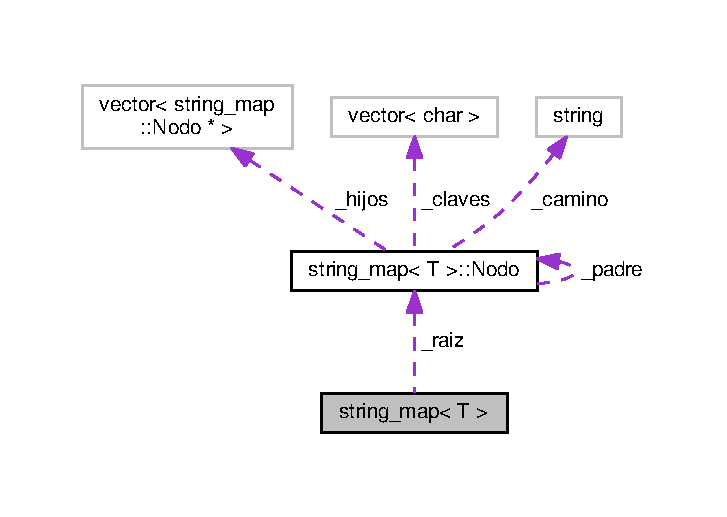
\includegraphics[width=349pt]{classstring__map__coll__graph}
\end{center}
\end{figure}
\subsection*{Clases}
\begin{DoxyCompactItemize}
\item 
class \hyperlink{classstring__map_1_1const__iterator}{const\-\_\-iterator}
\item 
class \hyperlink{classstring__map_1_1iterator}{iterator}
\item 
struct \hyperlink{structstring__map_1_1Nodo}{Nodo}
\end{DoxyCompactItemize}
\subsection*{Tipos públicos}
\begin{DoxyCompactItemize}
\item 
\hypertarget{classstring__map_ac6b29d74d0658db5938f53b66394d2ca}{typedef string {\bfseries key\-\_\-type}}\label{classstring__map_ac6b29d74d0658db5938f53b66394d2ca}

\item 
\hypertarget{classstring__map_a87309fe41124ea0f9f9fe22729e1fdf7}{typedef T {\bfseries mapped\-\_\-type}}\label{classstring__map_a87309fe41124ea0f9f9fe22729e1fdf7}

\item 
\hypertarget{classstring__map_aba7d0f8b84310cf46a990b404834074b}{typedef std\-::pair$<$ const \\*
key\-\_\-type, mapped\-\_\-type $>$ {\bfseries value\-\_\-type}}\label{classstring__map_aba7d0f8b84310cf46a990b404834074b}

\item 
\hypertarget{classstring__map_a91a355e52de423b8385b72caf553e3de}{typedef size\-\_\-t {\bfseries size\-\_\-type}}\label{classstring__map_a91a355e52de423b8385b72caf553e3de}

\end{DoxyCompactItemize}
\subsection*{Métodos públicos}
\begin{DoxyCompactItemize}
\item 
\hyperlink{classstring__map_acd7803d493b09db56e2e9022e526def7}{string\-\_\-map} ()
\begin{DoxyCompactList}\small\item\em Construye mapa vacio. \end{DoxyCompactList}\item 
\hyperlink{classstring__map_a37b201370c0a6a3c2aa488dedbc0a9d7}{$\sim$string\-\_\-map} ()
\begin{DoxyCompactList}\small\item\em Destruye mapa. \end{DoxyCompactList}\item 
\hyperlink{classstring__map_afa602ae4726c1dc0a562652107cdabfd}{string\-\_\-map} (const \hyperlink{classstring__map}{string\-\_\-map} \&)
\begin{DoxyCompactList}\small\item\em Constructor por copia. \end{DoxyCompactList}\item 
\hyperlink{classstring__map}{string\-\_\-map} \& \hyperlink{classstring__map_aa7099ce0e833b1d7b55990870d3cddac}{operator=} (const \hyperlink{classstring__map}{string\-\_\-map} \&)
\begin{DoxyCompactList}\small\item\em Operador de asignacion. \end{DoxyCompactList}\item 
bool \hyperlink{classstring__map_a424a95ef628cc97aeedae51f98ee2345}{operator==} (const \hyperlink{classstring__map}{string\-\_\-map} \&otro) const 
\begin{DoxyCompactList}\small\item\em Operadores de comparacion. \end{DoxyCompactList}\item 
\hypertarget{classstring__map_aaa9e3e8289202b72f1b0b7b0268c3fe7}{bool {\bfseries operator!=} (const \hyperlink{classstring__map}{string\-\_\-map} \&otro) const }\label{classstring__map_aaa9e3e8289202b72f1b0b7b0268c3fe7}

\item 
size\-\_\-type \hyperlink{classstring__map_a66402d4dcc1216dbcd32b0f182094a99}{count} (const key\-\_\-type \&key) const 
\begin{DoxyCompactList}\small\item\em Cantidad de apariciones de la clave (0 o 1) \end{DoxyCompactList}\item 
\hypertarget{classstring__map_af4943b5e157f925a5085852b1e3ffac1}{size\-\_\-t \hyperlink{classstring__map_af4943b5e157f925a5085852b1e3ffac1}{size} () const }\label{classstring__map_af4943b5e157f925a5085852b1e3ffac1}

\begin{DoxyCompactList}\small\item\em Devuelve cantidad de claves definidas. \end{DoxyCompactList}\item 
\hypertarget{classstring__map_a9a83f6f168f104c5d6c05c3fb989ad1f}{bool \hyperlink{classstring__map_a9a83f6f168f104c5d6c05c3fb989ad1f}{empty} () const }\label{classstring__map_a9a83f6f168f104c5d6c05c3fb989ad1f}

\begin{DoxyCompactList}\small\item\em devuelve true si \hyperlink{classstring__map_af4943b5e157f925a5085852b1e3ffac1}{size()} == 0 \end{DoxyCompactList}\item 
mapped\-\_\-type \& \hyperlink{classstring__map_a82bd8d05388e69e02a75980ef759e217}{operator\mbox{[}$\,$\mbox{]}} (const key\-\_\-type \&key)
\begin{DoxyCompactList}\small\item\em Acceso / definición de pares clave/valor. \end{DoxyCompactList}\item 
mapped\-\_\-type \& \hyperlink{classstring__map_afcc707f585755be24ffc4b06149f1cec}{at} (const key\-\_\-type \&key)
\begin{DoxyCompactList}\small\item\em Acceso a una clave sin modificar mapa. \end{DoxyCompactList}\item 
const mapped\-\_\-type \& \hyperlink{classstring__map_a26b3ded1c1736abff4580e994fab843e}{at} (const key\-\_\-type \&key) const 
\begin{DoxyCompactList}\small\item\em Acceso a una clave sin modificar mapa. \end{DoxyCompactList}\item 
\hypertarget{classstring__map_a5e0460b9c8c6f7c6e5f76e0112446842}{void \hyperlink{classstring__map_a5e0460b9c8c6f7c6e5f76e0112446842}{clear} ()}\label{classstring__map_a5e0460b9c8c6f7c6e5f76e0112446842}

\begin{DoxyCompactList}\small\item\em Vacia el mapa. \end{DoxyCompactList}\item 
\hyperlink{classstring__map_1_1iterator}{iterator} \hyperlink{classstring__map_aced2bd9493475515f3dc765a379484bd}{begin} ()
\begin{DoxyCompactList}\small\item\em iterador al primer par $<$clave,significado$>$ en orden lexicografico \end{DoxyCompactList}\item 
\hyperlink{classstring__map_1_1iterator}{iterator} \hyperlink{classstring__map_ab063b2f78945d192c5ef3ccc68db8e80}{end} ()
\begin{DoxyCompactList}\small\item\em iterador al fin de la coleccion \end{DoxyCompactList}\item 
\hypertarget{classstring__map_a978694b6ac9df86a1688d1e4a0642e52}{\hyperlink{classstring__map_1_1const__iterator}{const\-\_\-iterator} \hyperlink{classstring__map_a978694b6ac9df86a1688d1e4a0642e52}{begin} () const }\label{classstring__map_a978694b6ac9df86a1688d1e4a0642e52}

\begin{DoxyCompactList}\small\item\em Versiones const de begin/end. \end{DoxyCompactList}\item 
\hypertarget{classstring__map_a66b1f31d0b10c79f549d51e687ec5446}{\hyperlink{classstring__map_1_1const__iterator}{const\-\_\-iterator} {\bfseries end} () const }\label{classstring__map_a66b1f31d0b10c79f549d51e687ec5446}

\item 
\hyperlink{classstring__map_1_1iterator}{iterator} \hyperlink{classstring__map_abbe345fcf0ece43b416ea0e4699d95ed}{find} (const key\-\_\-type \&key)
\begin{DoxyCompactList}\small\item\em busca una clave \end{DoxyCompactList}\item 
\hyperlink{classstring__map_1_1const__iterator}{const\-\_\-iterator} \hyperlink{classstring__map_a4705d569ebabcfe6ecbe3a4c66958ce5}{find} (const key\-\_\-type \&key) const 
\begin{DoxyCompactList}\small\item\em busca una clave \end{DoxyCompactList}\item 
pair$<$ \hyperlink{classstring__map_1_1iterator}{iterator}, bool $>$ \hyperlink{classstring__map_a2fff1076bccd20802f03f72a92275b33}{insert} (const value\-\_\-type \&value)
\begin{DoxyCompactList}\small\item\em insercion \end{DoxyCompactList}\item 
size\-\_\-type \hyperlink{classstring__map_a978744cf6b1e5bccda86fd58e8cf5875}{erase} (const key\-\_\-type \&key)
\begin{DoxyCompactList}\small\item\em eliminar una clave \end{DoxyCompactList}\item 
\hyperlink{classstring__map_1_1iterator}{iterator} \hyperlink{classstring__map_aad96e9f05f2a7f4196331e0fcba3bae7}{erase} (\hyperlink{classstring__map_1_1iterator}{iterator} pos)
\begin{DoxyCompactList}\small\item\em eliminar una clave mediante irerador \end{DoxyCompactList}\item 
int \hyperlink{classstring__map_a06aa162a8803f84325b9b42391edeef2}{posicion} (vector$<$ char $>$ v, char c) const 
\begin{DoxyCompactList}\small\item\em Devuelve la posicion de c en v, v posee un tamaño acotado. \end{DoxyCompactList}\item 
bool \hyperlink{classstring__map_a6d32bfac880602723f942a29fdd56896}{igual\-De\-Nodo} (\hyperlink{structstring__map_1_1Nodo}{Nodo} \&n1, \hyperlink{structstring__map_1_1Nodo}{Nodo} \&n2) const 
\begin{DoxyCompactList}\small\item\em se fija si dos ramas son iguales \end{DoxyCompactList}\end{DoxyCompactItemize}
\subsection*{Atributos privados}
\begin{DoxyCompactItemize}
\item 
\hypertarget{classstring__map_a6ae83923332133a3d78a7c2405f3ac04}{\hyperlink{structstring__map_1_1Nodo}{Nodo} $\ast$ {\bfseries \-\_\-raiz}}\label{classstring__map_a6ae83923332133a3d78a7c2405f3ac04}

\item 
\hypertarget{classstring__map_aa883c09300422c5cfb8ab4d70386d3de}{size\-\_\-type {\bfseries \-\_\-tamano}}\label{classstring__map_aa883c09300422c5cfb8ab4d70386d3de}

\end{DoxyCompactItemize}
\subsection*{Amigas}
\begin{DoxyCompactItemize}
\item 
\hypertarget{classstring__map_a67171474c4da6cc8efe0c7fafefd2b2d}{class {\bfseries iterator}}\label{classstring__map_a67171474c4da6cc8efe0c7fafefd2b2d}

\item 
\hypertarget{classstring__map_ac220ce1c155db1ac44146c12d178056f}{class {\bfseries const\-\_\-iterator}}\label{classstring__map_ac220ce1c155db1ac44146c12d178056f}

\end{DoxyCompactItemize}


\subsection{Descripción detallada}
\subsubsection*{template$<$typename T$>$class string\-\_\-map$<$ T $>$}

Implementacion de map$<$string,\-T$>$ sobre Trie Asume de T\-:
\begin{DoxyItemize}
\item tiene constructor por copia
\item tiene operador ==
\item solo permite utilizar el operator\mbox{[}\mbox{]} si T tiene constructor por defecto 
\end{DoxyItemize}

\subsection{Documentación del constructor y destructor}
\hypertarget{classstring__map_acd7803d493b09db56e2e9022e526def7}{\index{string\-\_\-map@{string\-\_\-map}!string\-\_\-map@{string\-\_\-map}}
\index{string\-\_\-map@{string\-\_\-map}!string_map@{string\-\_\-map}}
\subsubsection[{string\-\_\-map}]{\setlength{\rightskip}{0pt plus 5cm}template$<$typename T $>$ {\bf string\-\_\-map}$<$ T $>$\-::{\bf string\-\_\-map} (
\begin{DoxyParamCaption}
{}
\end{DoxyParamCaption}
)}}\label{classstring__map_acd7803d493b09db56e2e9022e526def7}


Construye mapa vacio. 


\begin{DoxyDescription}
\item[Complejidad Temporal]$O$(1)
\end{DoxyDescription}\hypertarget{classstring__map_a37b201370c0a6a3c2aa488dedbc0a9d7}{\index{string\-\_\-map@{string\-\_\-map}!$\sim$string\-\_\-map@{$\sim$string\-\_\-map}}
\index{$\sim$string\-\_\-map@{$\sim$string\-\_\-map}!string_map@{string\-\_\-map}}
\subsubsection[{$\sim$string\-\_\-map}]{\setlength{\rightskip}{0pt plus 5cm}template$<$typename T $>$ {\bf string\-\_\-map}$<$ T $>$\-::$\sim${\bf string\-\_\-map} (
\begin{DoxyParamCaption}
{}
\end{DoxyParamCaption}
)}}\label{classstring__map_a37b201370c0a6a3c2aa488dedbc0a9d7}


Destruye mapa. 


\begin{DoxyDescription}
\item[Complejidad Temporal]$O$(sn $\ast$ S)
\end{DoxyDescription}\hypertarget{classstring__map_afa602ae4726c1dc0a562652107cdabfd}{\index{string\-\_\-map@{string\-\_\-map}!string\-\_\-map@{string\-\_\-map}}
\index{string\-\_\-map@{string\-\_\-map}!string_map@{string\-\_\-map}}
\subsubsection[{string\-\_\-map}]{\setlength{\rightskip}{0pt plus 5cm}template$<$typename T $>$ {\bf string\-\_\-map}$<$ T $>$\-::{\bf string\-\_\-map} (
\begin{DoxyParamCaption}
\item[{const {\bf string\-\_\-map}$<$ T $>$ \&}]{other}
\end{DoxyParamCaption}
)}}\label{classstring__map_afa602ae4726c1dc0a562652107cdabfd}


Constructor por copia. 


\begin{DoxyDescription}
\item[Complejidad Temporal]$O$(sn $\ast$ S)
\end{DoxyDescription}

\subsection{Documentación de las funciones miembro}
\hypertarget{classstring__map_afcc707f585755be24ffc4b06149f1cec}{\index{string\-\_\-map@{string\-\_\-map}!at@{at}}
\index{at@{at}!string_map@{string\-\_\-map}}
\subsubsection[{at}]{\setlength{\rightskip}{0pt plus 5cm}template$<$typename T $>$ {\bf string\-\_\-map}$<$ T $>$\-::mapped\-\_\-type \& {\bf string\-\_\-map}$<$ T $>$\-::at (
\begin{DoxyParamCaption}
\item[{const key\-\_\-type \&}]{key}
\end{DoxyParamCaption}
)}}\label{classstring__map_afcc707f585755be24ffc4b06149f1cec}


Acceso a una clave sin modificar mapa. 


\begin{DoxyParams}{Parámetros}
{\em key} & clave a acceder que debe existir previamente \\
\hline
\end{DoxyParams}
\begin{DoxyReturn}{Devuelve}
una referencia a la definicion.
\end{DoxyReturn}

\begin{DoxyDescription}
\item[Complejidad Temporal]$O$(S)
\end{DoxyDescription}\hypertarget{classstring__map_a26b3ded1c1736abff4580e994fab843e}{\index{string\-\_\-map@{string\-\_\-map}!at@{at}}
\index{at@{at}!string_map@{string\-\_\-map}}
\subsubsection[{at}]{\setlength{\rightskip}{0pt plus 5cm}template$<$typename T $>$ const {\bf string\-\_\-map}$<$ T $>$\-::mapped\-\_\-type \& {\bf string\-\_\-map}$<$ T $>$\-::at (
\begin{DoxyParamCaption}
\item[{const key\-\_\-type \&}]{key}
\end{DoxyParamCaption}
) const}}\label{classstring__map_a26b3ded1c1736abff4580e994fab843e}


Acceso a una clave sin modificar mapa. 


\begin{DoxyParams}{Parámetros}
{\em key} & clave a acceder que debe existir previamente \\
\hline
\end{DoxyParams}
\begin{DoxyReturn}{Devuelve}
una referencia const a la definicion.
\end{DoxyReturn}

\begin{DoxyDescription}
\item[Complejidad Temporal]$O$(S)
\end{DoxyDescription}\hypertarget{classstring__map_aced2bd9493475515f3dc765a379484bd}{\index{string\-\_\-map@{string\-\_\-map}!begin@{begin}}
\index{begin@{begin}!string_map@{string\-\_\-map}}
\subsubsection[{begin}]{\setlength{\rightskip}{0pt plus 5cm}template$<$typename T $>$ {\bf string\-\_\-map}$<$ T $>$\-::{\bf iterator} {\bf string\-\_\-map}$<$ T $>$\-::begin (
\begin{DoxyParamCaption}
{}
\end{DoxyParamCaption}
)}}\label{classstring__map_aced2bd9493475515f3dc765a379484bd}


iterador al primer par $<$clave,significado$>$ en orden lexicografico 

\begin{DoxyReturn}{Devuelve}
iterador al elemento o \hyperlink{classstring__map_ab063b2f78945d192c5ef3ccc68db8e80}{end()} si el mapa era vacio
\end{DoxyReturn}

\begin{DoxyDescription}
\item[Complejidad Temporal]$O$(S)
\end{DoxyDescription}\hypertarget{classstring__map_a66402d4dcc1216dbcd32b0f182094a99}{\index{string\-\_\-map@{string\-\_\-map}!count@{count}}
\index{count@{count}!string_map@{string\-\_\-map}}
\subsubsection[{count}]{\setlength{\rightskip}{0pt plus 5cm}template$<$typename T $>$ size\-\_\-t {\bf string\-\_\-map}$<$ T $>$\-::count (
\begin{DoxyParamCaption}
\item[{const key\-\_\-type \&}]{key}
\end{DoxyParamCaption}
) const}}\label{classstring__map_a66402d4dcc1216dbcd32b0f182094a99}


Cantidad de apariciones de la clave (0 o 1) 


\begin{DoxyParams}{Parámetros}
{\em key} & clave a buscar\\
\hline
\end{DoxyParams}

\begin{DoxyDescription}
\item[Complejidad Temporal]$O$(S)
\end{DoxyDescription}\hypertarget{classstring__map_ab063b2f78945d192c5ef3ccc68db8e80}{\index{string\-\_\-map@{string\-\_\-map}!end@{end}}
\index{end@{end}!string_map@{string\-\_\-map}}
\subsubsection[{end}]{\setlength{\rightskip}{0pt plus 5cm}template$<$typename T $>$ {\bf string\-\_\-map}$<$ T $>$\-::{\bf iterator} {\bf string\-\_\-map}$<$ T $>$\-::end (
\begin{DoxyParamCaption}
{}
\end{DoxyParamCaption}
)}}\label{classstring__map_ab063b2f78945d192c5ef3ccc68db8e80}


iterador al fin de la coleccion 


\begin{DoxyDescription}
\item[Complejidad Temporal]$O$(S)
\end{DoxyDescription}\hypertarget{classstring__map_a978744cf6b1e5bccda86fd58e8cf5875}{\index{string\-\_\-map@{string\-\_\-map}!erase@{erase}}
\index{erase@{erase}!string_map@{string\-\_\-map}}
\subsubsection[{erase}]{\setlength{\rightskip}{0pt plus 5cm}template$<$typename T $>$ {\bf string\-\_\-map}$<$ T $>$\-::size\-\_\-type {\bf string\-\_\-map}$<$ T $>$\-::erase (
\begin{DoxyParamCaption}
\item[{const key\-\_\-type \&}]{key}
\end{DoxyParamCaption}
)}}\label{classstring__map_a978744cf6b1e5bccda86fd58e8cf5875}


eliminar una clave 


\begin{DoxyParams}{Parámetros}
{\em key} & clave a eliminar \\
\hline
\end{DoxyParams}
\begin{DoxyReturn}{Devuelve}
cantidad de elementos eliminados
\end{DoxyReturn}

\begin{DoxyDescription}
\item[Complejidad Temporal]$O$(S)
\end{DoxyDescription}\hypertarget{classstring__map_aad96e9f05f2a7f4196331e0fcba3bae7}{\index{string\-\_\-map@{string\-\_\-map}!erase@{erase}}
\index{erase@{erase}!string_map@{string\-\_\-map}}
\subsubsection[{erase}]{\setlength{\rightskip}{0pt plus 5cm}template$<$typename T $>$ {\bf string\-\_\-map}$<$ T $>$\-::{\bf iterator} {\bf string\-\_\-map}$<$ T $>$\-::erase (
\begin{DoxyParamCaption}
\item[{{\bf iterator}}]{pos}
\end{DoxyParamCaption}
)}}\label{classstring__map_aad96e9f05f2a7f4196331e0fcba3bae7}


eliminar una clave mediante irerador 


\begin{DoxyParams}{Parámetros}
{\em pos} & iterador apuntando a clave a eliminar \\
\hline
\end{DoxyParams}
\begin{DoxyReturn}{Devuelve}
iterador apuntando el proximo de la clave eliminada (o \hyperlink{classstring__map_ab063b2f78945d192c5ef3ccc68db8e80}{end()} si era la ultima)
\end{DoxyReturn}

\begin{DoxyDescription}
\item[Complejidad Temporal]$O$(S)
\end{DoxyDescription}\hypertarget{classstring__map_abbe345fcf0ece43b416ea0e4699d95ed}{\index{string\-\_\-map@{string\-\_\-map}!find@{find}}
\index{find@{find}!string_map@{string\-\_\-map}}
\subsubsection[{find}]{\setlength{\rightskip}{0pt plus 5cm}template$<$typename T $>$ {\bf string\-\_\-map}$<$ T $>$\-::{\bf iterator} {\bf string\-\_\-map}$<$ T $>$\-::find (
\begin{DoxyParamCaption}
\item[{const key\-\_\-type \&}]{key}
\end{DoxyParamCaption}
)}}\label{classstring__map_abbe345fcf0ece43b416ea0e4699d95ed}


busca una clave 


\begin{DoxyParams}{Parámetros}
{\em key} & clave a buscar \\
\hline
\end{DoxyParams}
\begin{DoxyReturn}{Devuelve}
un iterador al par $<$clave, significado$>$
\end{DoxyReturn}

\begin{DoxyDescription}
\item[Complejidad Temporal]$O$(S)
\end{DoxyDescription}\hypertarget{classstring__map_a4705d569ebabcfe6ecbe3a4c66958ce5}{\index{string\-\_\-map@{string\-\_\-map}!find@{find}}
\index{find@{find}!string_map@{string\-\_\-map}}
\subsubsection[{find}]{\setlength{\rightskip}{0pt plus 5cm}template$<$typename T $>$ {\bf string\-\_\-map}$<$ T $>$\-::{\bf const\-\_\-iterator} {\bf string\-\_\-map}$<$ T $>$\-::find (
\begin{DoxyParamCaption}
\item[{const key\-\_\-type \&}]{key}
\end{DoxyParamCaption}
) const}}\label{classstring__map_a4705d569ebabcfe6ecbe3a4c66958ce5}


busca una clave 


\begin{DoxyParams}{Parámetros}
{\em key} & clave a buscar \\
\hline
\end{DoxyParams}
\begin{DoxyReturn}{Devuelve}
un iterador const al par $<$clave, significado$>$
\end{DoxyReturn}

\begin{DoxyDescription}
\item[Complejidad Temporal]$O$(S)
\end{DoxyDescription}\hypertarget{classstring__map_a6d32bfac880602723f942a29fdd56896}{\index{string\-\_\-map@{string\-\_\-map}!igual\-De\-Nodo@{igual\-De\-Nodo}}
\index{igual\-De\-Nodo@{igual\-De\-Nodo}!string_map@{string\-\_\-map}}
\subsubsection[{igual\-De\-Nodo}]{\setlength{\rightskip}{0pt plus 5cm}template$<$typename T$>$ bool {\bf string\-\_\-map}$<$ T $>$\-::igual\-De\-Nodo (
\begin{DoxyParamCaption}
\item[{{\bf Nodo} \&}]{n1, }
\item[{{\bf Nodo} \&}]{n2}
\end{DoxyParamCaption}
) const}}\label{classstring__map_a6d32bfac880602723f942a29fdd56896}


se fija si dos ramas son iguales 


\begin{DoxyParams}{Parámetros}
{\em n1} & \hyperlink{structstring__map_1_1Nodo}{Nodo} \\
\hline
{\em n2} & \hyperlink{structstring__map_1_1Nodo}{Nodo} \\
\hline
\end{DoxyParams}
\begin{DoxyReturn}{Devuelve}
devuelve true si n1 == n2
\end{DoxyReturn}

\begin{DoxyDescription}
\item[Complejidad Temporal]$O$(cant nodos)
\end{DoxyDescription}\hypertarget{classstring__map_a2fff1076bccd20802f03f72a92275b33}{\index{string\-\_\-map@{string\-\_\-map}!insert@{insert}}
\index{insert@{insert}!string_map@{string\-\_\-map}}
\subsubsection[{insert}]{\setlength{\rightskip}{0pt plus 5cm}template$<$typename T$>$ pair$<$ typename {\bf string\-\_\-map}$<$ T $>$\-::{\bf iterator}, bool $>$ {\bf string\-\_\-map}$<$ T $>$\-::insert (
\begin{DoxyParamCaption}
\item[{const value\-\_\-type \&}]{value}
\end{DoxyParamCaption}
)}}\label{classstring__map_a2fff1076bccd20802f03f72a92275b33}


insercion 


\begin{DoxyParams}{Parámetros}
{\em value} & par $<$clave,significado$>$ a insertar \\
\hline
\end{DoxyParams}
\begin{DoxyReturn}{Devuelve}
un par con un iterador al par clave-\/significado agregado o modificado y un bool que indica si la clave se insertó como una clave nueva.
\end{DoxyReturn}

\begin{DoxyDescription}
\item[Complejidad Temporal]$O$(S + copy(value\-\_\-type))
\end{DoxyDescription}\hypertarget{classstring__map_aa7099ce0e833b1d7b55990870d3cddac}{\index{string\-\_\-map@{string\-\_\-map}!operator=@{operator=}}
\index{operator=@{operator=}!string_map@{string\-\_\-map}}
\subsubsection[{operator=}]{\setlength{\rightskip}{0pt plus 5cm}template$<$typename T $>$ {\bf string\-\_\-map}$<$ T $>$ \& {\bf string\-\_\-map}$<$ T $>$\-::operator= (
\begin{DoxyParamCaption}
\item[{const {\bf string\-\_\-map}$<$ T $>$ \&}]{other}
\end{DoxyParamCaption}
)}}\label{classstring__map_aa7099ce0e833b1d7b55990870d3cddac}


Operador de asignacion. 


\begin{DoxyDescription}
\item[Complejidad Temporal]$O$(sn $\ast$ S)
\end{DoxyDescription}\hypertarget{classstring__map_a424a95ef628cc97aeedae51f98ee2345}{\index{string\-\_\-map@{string\-\_\-map}!operator==@{operator==}}
\index{operator==@{operator==}!string_map@{string\-\_\-map}}
\subsubsection[{operator==}]{\setlength{\rightskip}{0pt plus 5cm}template$<$typename T $>$ bool {\bf string\-\_\-map}$<$ T $>$\-::operator== (
\begin{DoxyParamCaption}
\item[{const {\bf string\-\_\-map}$<$ T $>$ \&}]{otro}
\end{DoxyParamCaption}
) const}}\label{classstring__map_a424a95ef628cc97aeedae51f98ee2345}


Operadores de comparacion. 


\begin{DoxyDescription}
\item[Complejidad Temporal]$O$(sn $\ast$ S)
\end{DoxyDescription}\hypertarget{classstring__map_a82bd8d05388e69e02a75980ef759e217}{\index{string\-\_\-map@{string\-\_\-map}!operator\mbox{[}$\,$\mbox{]}@{operator[]}}
\index{operator\mbox{[}$\,$\mbox{]}@{operator[]}!string_map@{string\-\_\-map}}
\subsubsection[{operator[]}]{\setlength{\rightskip}{0pt plus 5cm}template$<$typename T $>$ {\bf string\-\_\-map}$<$ T $>$\-::mapped\-\_\-type \& {\bf string\-\_\-map}$<$ T $>$\-::operator\mbox{[}$\,$\mbox{]} (
\begin{DoxyParamCaption}
\item[{const key\-\_\-type \&}]{key}
\end{DoxyParamCaption}
)}}\label{classstring__map_a82bd8d05388e69e02a75980ef759e217}


Acceso / definición de pares clave/valor. 


\begin{DoxyParams}{Parámetros}
{\em key} & clave a acceder, si no existe, se crea \\
\hline
\end{DoxyParams}
\begin{DoxyReturn}{Devuelve}
una referencia a la definicion.
\end{DoxyReturn}

\begin{DoxyDescription}
\item[Complejidad Temporal]$O$(S)
\end{DoxyDescription}\hypertarget{classstring__map_a06aa162a8803f84325b9b42391edeef2}{\index{string\-\_\-map@{string\-\_\-map}!posicion@{posicion}}
\index{posicion@{posicion}!string_map@{string\-\_\-map}}
\subsubsection[{posicion}]{\setlength{\rightskip}{0pt plus 5cm}template$<$typename T $>$ int {\bf string\-\_\-map}$<$ T $>$\-::posicion (
\begin{DoxyParamCaption}
\item[{vector$<$ char $>$}]{v, }
\item[{char}]{c}
\end{DoxyParamCaption}
) const}}\label{classstring__map_a06aa162a8803f84325b9b42391edeef2}


Devuelve la posicion de c en v, v posee un tamaño acotado. 


\begin{DoxyParams}{Parámetros}
{\em v} & Vector \\
\hline
{\em c} & Char \\
\hline
\end{DoxyParams}
\begin{DoxyPrecond}{Precondición}
c $\in$ v 
\end{DoxyPrecond}
\begin{DoxyReturn}{Devuelve}
posicion en la cual se encuentra c
\end{DoxyReturn}

\begin{DoxyDescription}
\item[Complejidad Temporal]$O$(1)
\end{DoxyDescription}

La documentación para esta clase fue generada a partir de los siguientes ficheros\-:\begin{DoxyCompactItemize}
\item 
src/string\-\_\-map.\-h\item 
src/string\-\_\-map.\-hpp\end{DoxyCompactItemize}

\hypertarget{classTabla}{\section{Referencia de la Clase Tabla}
\label{classTabla}\index{Tabla@{Tabla}}
}


Representa una tabla de una base de datos.  




{\ttfamily \#include $<$Tabla.\-h$>$}



Diagrama de colaboración para Tabla\-:\nopagebreak
\begin{figure}[H]
\begin{center}
\leavevmode
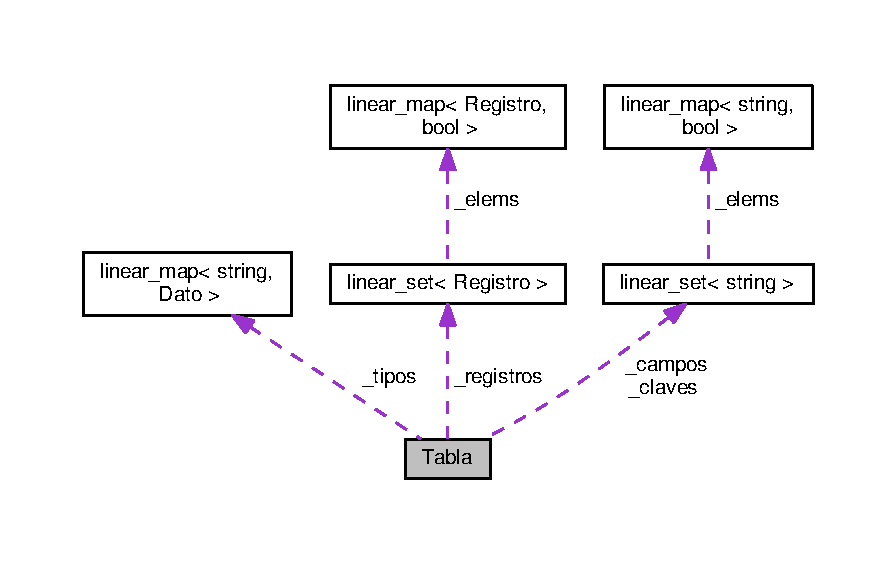
\includegraphics[width=350pt]{classTabla__coll__graph}
\end{center}
\end{figure}
\subsection*{Clases}
\begin{DoxyCompactItemize}
\item 
class \hyperlink{classTabla_1_1const__iterador__registros}{const\-\_\-iterador\-\_\-registros}
\begin{DoxyCompactList}\small\item\em Iterador de los registros de una tabla. \end{DoxyCompactList}\end{DoxyCompactItemize}
\subsection*{Métodos públicos}
\begin{DoxyCompactItemize}
\item 
\hyperlink{classTabla_a5a7be353082561e06a877b2255c0ea5c}{Tabla} (const \hyperlink{classlinear__set}{linear\-\_\-set}$<$ string $>$ \&\hyperlink{classTabla_aaea7c833fd1f68742785482809c8667a}{claves}, const vector$<$ string $>$ \&\hyperlink{classTabla_a3436d172652646a83d8035d1c68b9073}{campos}, const vector$<$ \hyperlink{classDato}{Dato} $>$ \&tipos)
\begin{DoxyCompactList}\small\item\em Inicializa una tabla sin registros y con la descripción parámetro. \end{DoxyCompactList}\item 
\hyperlink{classTabla_1_1const__iterador__registros}{const\-\_\-iterador\-\_\-registros} \hyperlink{classTabla_a99345e41702e7e9984732c6f3672e386}{agregar\-Registro} (const \hyperlink{classRegistro}{Registro} \&r)
\begin{DoxyCompactList}\small\item\em Inserta un nuevo registro en la tabla. \end{DoxyCompactList}\item 
const \hyperlink{classlinear__set}{linear\-\_\-set}$<$ string $>$ \& \hyperlink{classTabla_a3436d172652646a83d8035d1c68b9073}{campos} () const 
\begin{DoxyCompactList}\small\item\em Campos de la tabla. \end{DoxyCompactList}\item 
const \hyperlink{classDato}{Dato} \& \hyperlink{classTabla_a256a50a84ffbf43b570c568bcaf5f52f}{tipo\-Campo} (const string \&campo) const 
\begin{DoxyCompactList}\small\item\em Tipo del campo parámetro para la tabla. \end{DoxyCompactList}\item 
const \hyperlink{classlinear__set}{linear\-\_\-set}$<$ string $>$ \& \hyperlink{classTabla_aaea7c833fd1f68742785482809c8667a}{claves} () const 
\begin{DoxyCompactList}\small\item\em Subconjunto de campos que son clave. \end{DoxyCompactList}\item 
\hypertarget{classTabla_a7bcdeb00d2fe040e454468d526cce66c}{const \hyperlink{classlinear__set}{linear\-\_\-set}$<$ \hyperlink{classRegistro}{Registro} $>$ \& {\bfseries registros} () const }\label{classTabla_a7bcdeb00d2fe040e454468d526cce66c}

\item 
\hypertarget{classTabla_ae25724a86075dd5121b07446c92e94c6}{int {\bfseries cant\-\_\-registros} () const }\label{classTabla_ae25724a86075dd5121b07446c92e94c6}

\item 
\hyperlink{classTabla_1_1const__iterador__registros}{const\-\_\-iterador\-\_\-registros} \hyperlink{classTabla_aafc1aedd4c2c222387591c3b772d56a9}{registros\-\_\-begin} () const 
\begin{DoxyCompactList}\small\item\em Iterador al inicio de los registros de la tabla. \end{DoxyCompactList}\item 
\hyperlink{classTabla_1_1const__iterador__registros}{const\-\_\-iterador\-\_\-registros} \hyperlink{classTabla_ac736bbd3065cc25c36ef258fcddaea50}{registros\-\_\-end} () const 
\begin{DoxyCompactList}\small\item\em Iterador al final de los registros de la tabla. \end{DoxyCompactList}\end{DoxyCompactItemize}
\subsection*{Atributos privados}
\begin{Indent}{\bf Representación}\par
{\em rep\-: tabla $\to$ bool\par
rep(t) $\equiv$
\begin{DoxyItemize}
\item $\lnot$ $\emptyset$?(\-\_\-claves) $\land$
\item \-\_\-claves $\subseteq$ \-\_\-campos $\land$
\item \-\_\-campos = claves(\-\_\-tipos) $\land$
\item $\forall$ (r \-: registro) r $\in$ \-\_\-registros $\Rightarrow$ (
\begin{DoxyItemize}
\item campos(r) = \-\_\-campos
\item $\forall$ (c \-: campo) c $\in$ \-\_\-campos $\Rightarrow$ Nat?(valor(c, r)) = Nat?(obtener(c, \-\_\-tipos))
\item no se repiten claves $\equiv$ $\forall$ (r' \-: registro) r $\in$ (\-\_\-registros -\/ \{r\}) $\Rightarrow$ $\lnot$ hay\-Coincidencia(r, \-\_\-claves, \-\_\-registros)
\end{DoxyItemize}
\item )
\end{DoxyItemize}

abs\-: tabla $\to$ \hyperlink{classTabla}{Tabla}\par
abs(t) $\equiv$ t' $|$
\begin{DoxyItemize}
\item campos(t') = \-\_\-campos $\land$
\item claves(t') = \-\_\-claves $\land$
\item $\forall$ (c \-: string) c  \-\_\-campos $\Rightarrow$ tipo\-Campo(c, r') = Nat?(obtener(c, \-\_\-tipos)) $\land$
\item registros(t') = \-\_\-registros 
\end{DoxyItemize}}\begin{DoxyCompactItemize}
\item 
\hypertarget{classTabla_a3fc11c070caf35a44a23724a6a5bae92}{\hyperlink{classlinear__set}{linear\-\_\-set}$<$ string $>$ {\bfseries \-\_\-claves}}\label{classTabla_a3fc11c070caf35a44a23724a6a5bae92}

\item 
\hypertarget{classTabla_ac527baaf100aea820dd4d1687b0f2378}{\hyperlink{classlinear__set}{linear\-\_\-set}$<$ string $>$ {\bfseries \-\_\-campos}}\label{classTabla_ac527baaf100aea820dd4d1687b0f2378}

\item 
\hypertarget{classTabla_af3bc6468c890f3c0ea110f45377abf51}{\hyperlink{classlinear__map}{linear\-\_\-map}$<$ string, \hyperlink{classDato}{Dato} $>$ {\bfseries \-\_\-tipos}}\label{classTabla_af3bc6468c890f3c0ea110f45377abf51}

\item 
\hypertarget{classTabla_a28b3aa83e48d95fbeb5a6308a58defcc}{\hyperlink{classlinear__set}{linear\-\_\-set}$<$ \hyperlink{classRegistro}{Registro} $>$ {\bfseries \-\_\-registros}}\label{classTabla_a28b3aa83e48d95fbeb5a6308a58defcc}

\end{DoxyCompactItemize}
\end{Indent}


\subsection{Descripción detallada}
Representa una tabla de una base de datos. 

Una tabla es una colección de registros que cumplen la descripción de la misma. La descripción de una tabla consiste en una serie de nombres que describen los campos y un tipo para cada campo que explicita el tipo de dato que un registro puede tener en ese campo.

La descripción también selecciona un subconjunto de los campos como  claves. Dada las claves, una tabla no puede tener dos registros con los mismos valores para todos los campos claves.

{\bfseries se explica con} T\-A\-D \hyperlink{classTabla}{Tabla} 

\subsection{Documentación del constructor y destructor}
\hypertarget{classTabla_a5a7be353082561e06a877b2255c0ea5c}{\index{Tabla@{Tabla}!Tabla@{Tabla}}
\index{Tabla@{Tabla}!Tabla@{Tabla}}
\subsubsection[{Tabla}]{\setlength{\rightskip}{0pt plus 5cm}Tabla\-::\-Tabla (
\begin{DoxyParamCaption}
\item[{const {\bf linear\-\_\-set}$<$ string $>$ \&}]{claves, }
\item[{const vector$<$ string $>$ \&}]{campos, }
\item[{const vector$<$ {\bf Dato} $>$ \&}]{tipos}
\end{DoxyParamCaption}
)}}\label{classTabla_a5a7be353082561e06a877b2255c0ea5c}


Inicializa una tabla sin registros y con la descripción parámetro. 


\begin{DoxyParams}{Parámetros}
{\em claves} & Subconjunto de los campos que son claves. \\
\hline
{\em campos} & Conjunto de nombres de claves. El órden se corresponde con el de datos \\
\hline
{\em tipos} & Conjunto de datos cuyo tipo define el tipo admisible en cada campo. El valor de los datos se ignora.\\
\hline
\end{DoxyParams}
\begin{DoxyPrecond}{Precondición}
$\lnot$ $\emptyset$ ?(c) $\land$ $\forall$ (c\-: campo) c  claves $\Rightarrow$ esta?(c, campos) $\land$ long(campos) = long(tipos) $\land$ sin\-Repetidos(campos) 
\end{DoxyPrecond}
\begin{DoxyPostcond}{Postcondición}
{\bfseries res} = nueva\-Tabla(claves, nuevo\-Registro(campos, tipos))
\end{DoxyPostcond}

\begin{DoxyDescription}
\item[Complejidad Temporal]$O$(long(campos) $\ast$ (copy(campo) + copy(dato)))
\end{DoxyDescription}

\subsection{Documentación de las funciones miembro}
\hypertarget{classTabla_a99345e41702e7e9984732c6f3672e386}{\index{Tabla@{Tabla}!agregar\-Registro@{agregar\-Registro}}
\index{agregar\-Registro@{agregar\-Registro}!Tabla@{Tabla}}
\subsubsection[{agregar\-Registro}]{\setlength{\rightskip}{0pt plus 5cm}{\bf Tabla\-::const\-\_\-iterador\-\_\-registros} Tabla\-::agregar\-Registro (
\begin{DoxyParamCaption}
\item[{const {\bf Registro} \&}]{r}
\end{DoxyParamCaption}
)}}\label{classTabla_a99345e41702e7e9984732c6f3672e386}


Inserta un nuevo registro en la tabla. 


\begin{DoxyParams}{Parámetros}
{\em r} & \hyperlink{classRegistro}{Registro} a agregar\\
\hline
\end{DoxyParams}
\begin{DoxyPrecond}{Precondición}
t = {\bfseries this} $\land$ campos(r) = campos(t) $\land$ puedo\-Insertar?(r, t) 
\end{DoxyPrecond}
\begin{DoxyPostcond}{Postcondición}
{\bfseries this} = agregar\-Registro(r, t) $\land$ {\bfseries res} apunta al registro recién agregado.
\end{DoxyPostcond}

\begin{DoxyDescription}
\item[Complejidad Temporal]$O$(copy(registro))
\end{DoxyDescription}\hypertarget{classTabla_a3436d172652646a83d8035d1c68b9073}{\index{Tabla@{Tabla}!campos@{campos}}
\index{campos@{campos}!Tabla@{Tabla}}
\subsubsection[{campos}]{\setlength{\rightskip}{0pt plus 5cm}const {\bf linear\-\_\-set}$<$ string $>$ \& Tabla\-::campos (
\begin{DoxyParamCaption}
{}
\end{DoxyParamCaption}
) const}}\label{classTabla_a3436d172652646a83d8035d1c68b9073}


Campos de la tabla. 

El conjunto se devuelve por referencia no-\/modificable

\begin{DoxyPrecond}{Precondición}
true 
\end{DoxyPrecond}
\begin{DoxyPostcond}{Postcondición}
{\bfseries res} = campos({\bfseries this})
\end{DoxyPostcond}

\begin{DoxyDescription}
\item[Complejidad Temporal]$O$(1)
\end{DoxyDescription}\hypertarget{classTabla_aaea7c833fd1f68742785482809c8667a}{\index{Tabla@{Tabla}!claves@{claves}}
\index{claves@{claves}!Tabla@{Tabla}}
\subsubsection[{claves}]{\setlength{\rightskip}{0pt plus 5cm}const {\bf linear\-\_\-set}$<$ string $>$ \& Tabla\-::claves (
\begin{DoxyParamCaption}
{}
\end{DoxyParamCaption}
) const}}\label{classTabla_aaea7c833fd1f68742785482809c8667a}


Subconjunto de campos que son clave. 

El conjunto se devuelve por referencia no-\/modificable.

\begin{DoxyPrecond}{Precondición}
true 
\end{DoxyPrecond}
\begin{DoxyPostcond}{Postcondición}
{\bfseries res} = claves({\bfseries this})
\end{DoxyPostcond}

\begin{DoxyDescription}
\item[Complejidad Temporal]$O$(1)
\end{DoxyDescription}\hypertarget{classTabla_aafc1aedd4c2c222387591c3b772d56a9}{\index{Tabla@{Tabla}!registros\-\_\-begin@{registros\-\_\-begin}}
\index{registros\-\_\-begin@{registros\-\_\-begin}!Tabla@{Tabla}}
\subsubsection[{registros\-\_\-begin}]{\setlength{\rightskip}{0pt plus 5cm}{\bf Tabla\-::const\-\_\-iterador\-\_\-registros} Tabla\-::registros\-\_\-begin (
\begin{DoxyParamCaption}
{}
\end{DoxyParamCaption}
) const}}\label{classTabla_aafc1aedd4c2c222387591c3b772d56a9}


Iterador al inicio de los registros de la tabla. 

El iterador resultado es conformante con \href{http://en.cppreference.com/w/cpp/concept/InputIterator}{\tt std\-::\-Input\-Iterator}

\begin{DoxyPrecond}{Precondición}
true 
\end{DoxyPrecond}
\begin{DoxyPostcond}{Postcondición}
El iterador {\bfseries res} recorre los registros de la tabla en un orden no definido.
\end{DoxyPostcond}

\begin{DoxyDescription}
\item[Complejidad Temporal]$O$(1)
\end{DoxyDescription}\hypertarget{classTabla_ac736bbd3065cc25c36ef258fcddaea50}{\index{Tabla@{Tabla}!registros\-\_\-end@{registros\-\_\-end}}
\index{registros\-\_\-end@{registros\-\_\-end}!Tabla@{Tabla}}
\subsubsection[{registros\-\_\-end}]{\setlength{\rightskip}{0pt plus 5cm}{\bf Tabla\-::const\-\_\-iterador\-\_\-registros} Tabla\-::registros\-\_\-end (
\begin{DoxyParamCaption}
{}
\end{DoxyParamCaption}
) const}}\label{classTabla_ac736bbd3065cc25c36ef258fcddaea50}


Iterador al final de los registros de la tabla. 

El iterador resultado es conformante con \href{http://en.cppreference.com/w/cpp/concept/InputIterator}{\tt std\-::\-Input\-Iterator}

\begin{DoxyPrecond}{Precondición}
true 
\end{DoxyPrecond}
\begin{DoxyPostcond}{Postcondición}
El iterador {\bfseries res} apunta al lugar-\/pasando-\/el-\/último de los registros de la tabla. Puede utilizarse para comparar con otro \hyperlink{classTabla_1_1const__iterador__registros}{const\-\_\-iterador\-\_\-registros} para saber si se llegó al final de la iteración.
\end{DoxyPostcond}

\begin{DoxyDescription}
\item[Complejidad Temporal]$O$(1)
\end{DoxyDescription}\hypertarget{classTabla_a256a50a84ffbf43b570c568bcaf5f52f}{\index{Tabla@{Tabla}!tipo\-Campo@{tipo\-Campo}}
\index{tipo\-Campo@{tipo\-Campo}!Tabla@{Tabla}}
\subsubsection[{tipo\-Campo}]{\setlength{\rightskip}{0pt plus 5cm}const {\bf Dato} \& Tabla\-::tipo\-Campo (
\begin{DoxyParamCaption}
\item[{const string \&}]{campo}
\end{DoxyParamCaption}
) const}}\label{classTabla_a256a50a84ffbf43b570c568bcaf5f52f}


Tipo del campo parámetro para la tabla. 

El dato se devuelve por referencia no-\/modificable. El dato se utiliza solo para representar el tipo. Su valor se ignora.

\begin{DoxyPrecond}{Precondición}
campo $\in$ campos({\bfseries this}) 
\end{DoxyPrecond}
\begin{DoxyPostcond}{Postcondición}
tipo\-Campo(campo, {\bfseries this})
\end{DoxyPostcond}

\begin{DoxyDescription}
\item[Complejidad Temporal]$O$(\#(campos({\bfseries this})) $\ast$ cmp(campo)
\end{DoxyDescription}

La documentación para esta clase fue generada a partir de los siguientes ficheros\-:\begin{DoxyCompactItemize}
\item 
src/Tabla.\-h\item 
src/Tabla.\-cpp\end{DoxyCompactItemize}

%--- End generated contents ---

% Index
\newpage
\phantomsection
\addcontentsline{toc}{chapter}{Índice}
\printindex

\end{document}
